\documentclass[11pt,a4paper]{article}

\usepackage[margin=2.5cm]{geometry}
\usepackage{amsmath,amssymb}
\usepackage{graphicx}
\usepackage{booktabs}
\usepackage{caption}
\usepackage[numbers,sort&compress]{natbib}
\usepackage{xcolor}
\definecolor{linkcol}{RGB}{25,60,130}
\usepackage[colorlinks=true,linkcolor=linkcol,citecolor=linkcol,urlcolor=linkcol]{hyperref}

\captionsetup{font=small,labelfont=bf}
\setlength{\emergencystretch}{3em}
\sloppy
% let floats pack more tightly, so the paper does not run to float pages
\renewcommand{\topfraction}{0.92}
\renewcommand{\bottomfraction}{0.85}
\renewcommand{\textfraction}{0.06}
\renewcommand{\floatpagefraction}{0.85}
\setlength{\floatsep}{10pt plus 2pt minus 2pt}
\setlength{\textfloatsep}{12pt plus 2pt minus 3pt}
\setlength{\intextsep}{10pt plus 2pt minus 2pt}
\graphicspath{{figures/}}

\newcommand{\um}{\ensuremath{\,\mu\mathrm{m}}}
\newcommand{\mm}{\ensuremath{\,\mathrm{mm}}}
\newcommand{\qop}{\ensuremath{\mathrm{qop}}}

% ---------------------------------------------------------------------------
% main.tex is the single authoritative source of this paper.  There is no
% other copy of the body text: the per-section drafts it was assembled from
% were deleted once this file became authoritative.  Edit main.tex.
% ---------------------------------------------------------------------------

% ---------------------------------------------------------------------------
\title{One network, chained to itself across the LHCb magnet:\\
a label-free extrapolator trained by what an error costs}

\author{George William Scriven\thanks{george.w.scriven@gmail.com}\\[2pt]
\normalsize Maastricht University, Maastricht, The Netherlands\\
\normalsize Hasselt University, Hasselt, Belgium\\
\normalsize Nikhef, Amsterdam, The Netherlands}

\date{\today}

\begin{document}
\maketitle

\begin{abstract}
Track reconstruction in LHCb calls an extrapolator, the routine that transports
a track state from one detector plane to another, millions of
times a second; crossing the spectrometer magnet is its most expensive step.
The first paper of this programme~\citep{scriven2026lhcb1} built a label-free
surrogate for the field-propagation part of the job from the
discrete-time construction of Raissi, Perdikaris and
Karniadakis~\citep{raissi2019}, and left one failure: inside a network serving
every kind of step, the single $5178\mm$ crossing sat a factor $22$ above the
scheme it was trained to solve. Here I cut the crossing into $N$ equal steps,
train \emph{one} network to take a step of length $\Delta z = L/N$ wherever it
starts, and apply it to its own output $N$ times; the network's outputs are
written as a correction to the straight line, not as the stage states directly.
The construction stays label-free: the training signal is the reconstruction
residual of a $q$-stage Gauss--Legendre collocation step evaluated in the
measured field map, and no reference trajectory enters the objective. On
$1452$ held-out tracks from an official LHCb simulation sample, chaining
removes the discretisation: the same scheme solved exactly and chained $64$
times sits $0.147\um$ from a sixth-order reference, while the trained chains of
$64$ steps or more sit between $137$ and $246\um$, limited by their
optimisation and by the accumulation. The experiment is a change of objective. An audit of that loss
finds it spending $89.8$ per cent
of itself on $3$--$8$ GeV tracks, $1.23$ per cent on the $10$--$50$ GeV region
of interest and $0.65$ per cent on the quarter of the crossing where an error
costs most. Replacing it with a loss that measures every residual
by the displacement it would cause at the far side of the magnet, as a fraction
of that track's own bend and with the region of interest weighted up --- built
from the network's inputs and the field map alone --- moves those three shares
to $38.3$, $47.0$ and $23.3$ per cent. At $N = 64$, $q = 2$,
$\Delta z = 80.9\mm$ the median endpoint error falls from $145.7$ to $88.8\um$,
the error inside the weighted window from $108.1$ to $24.8\um$, a factor
$4.37$, and the median per-step slope error from $1.30\times10^{-6}$ to
$7.34\times10^{-7}$. Both pre-registered conditions are met, though the
second is weak: the pooled-loss counterpart has since cleared it too. The
price is specific: below the crossover between $3$--$8$ and $8$--$20$ GeV the
reweighted network is worse in five of six comparisons (these counts run over
three matched pairs, and two of the three pooled counterparts had not reached
the plateau rule), the median below
$3$ GeV rises from $353.7$ to $615.1\um$, the $95$th percentile from $898$ to
$1399\um$, and the fraction beyond a millimetre from $4.41$ to
$7.16$ per cent. The whole of the gain is in the bending plane, the vertical
plane does not move, and what remains is \emph{more} coherent along the chain
in all six matched comparisons, $0.31$ to $0.53$ against the $0.0625$ to
$0.125$ of independent steps. Shortening the step from $80.9$ to $20.2\mm$
halves each step's error and does not improve the crossing. Against
the simulated particle, network and reference are indistinguishable: the three
cost-weighted networks sit $12.5$ to $25.2$ times closer to one another than
either is to the truth in every band from $<3$ to $20$--$50$ GeV and in the
loss window, because neither models the material. In the thirty-track
$>50$ GeV band the pooled networks instead approach the reference-to-truth
gap, the ratio falling to $0.85$.
\end{abstract}

\tableofcontents

% ===========================================================================
\section{Introduction}
\label{sec:intro}

This paper reports one experiment and the machinery needed to read it. A single
small neural network is trained to take one fixed step in $z$ across the LHCb
magnet, and is then applied to its own output as many times as it takes to
cross. It is trained without labels: it is never shown where a particle went,
only required to satisfy the algebra of an implicit Runge--Kutta step evaluated
in the measured magnetic field. The experiment is the loss. The same network,
at the same three step lengths, is trained twice, once under the loss the
construction comes with and once under a loss that measures every residual by
what that residual would cost at the far side of the magnet, and the two are
compared on the same held-out tracks by the same statistics.

I have written this section, and the theory section that follows it, for a
reader with no prior exposure to LHCb, to track fitting, or to
physics-informed neural networks. Every term is defined at first use and every
symbol is introduced in a ``where \dots'' clause beside the equation it appears
in. Section~\ref{sec:intro-cost} says what an extrapolator is and why its cost
matters. Section~\ref{sec:intro-paper1} states what the first study of this
programme~\citep{scriven2026lhcb1} established and the one failure it left
behind. Section~\ref{sec:intro-selfchain} states the design change this paper
makes in response. Section~\ref{sec:intro-questions} sets the two questions the
paper answers, and Section~\ref{sec:intro-roadmap} is the road map.

\subsection{The extrapolator and why it is the cost in the fit}
\label{sec:intro-cost}

LHCb is one of the four large experiments at the Large Hadron Collider at CERN,
rebuilt for the current data-taking period as a fully software-triggered
forward spectrometer~\citep{lhcb2024upgrade}. Protons are brought into
collision at its centre tens of millions of times a second, each collision
sprays out charged particles, and the detector's job is to work out which
particles were produced and where they came from. It does that by placing
layers of position-sensitive silicon and scintillating fibre along the beam
direction, so that a particle passing through leaves a series of measured
points, called \textbf{hits}. A \textbf{track} is the reconstructed path of one
charged particle through the detector, fitted to those hits.

Three groups of layers matter here. The vertex detector surrounds the collision
point. The \textbf{Upstream Tracker} is a set of four silicon planes
immediately in front of the magnet. The \textbf{scintillating-fibre tracker},
usually written SciFi, is twelve layers immediately behind it. Between the
second and the third sits a large dipole magnet whose field is roughly
vertical and about one tesla at its strongest. A charged particle passing
through a magnetic field is deflected, and the deflection is inversely
proportional to its momentum: fast particles are barely bent, slow particles
are bent a great deal. The magnet is therefore the instrument that measures
momentum. It is also the reason the geometry of a track is not a straight line,
and the reason this paper exists.

Throughout, $z$ runs along the beam direction, $x$ is horizontal and transverse
to the beam, and $y$ is vertical. Because LHCb detects particles that go
forward at small angles to the beam, every particle of interest moves
monotonically in $z$, and it is convenient to describe a track not as a
function of time but as a function of $z$.

A \textbf{track state} is the complete description of a track at one value of
$z$. It is a list of five numbers,
%
\begin{equation}
  S = (x,\ y,\ t_x,\ t_y,\ \qop),
  \label{eq:state}
\end{equation}
%
where $x$ and $y$ are the transverse positions of the track at that $z$, in
millimetres; $t_x = \mathrm{d}x/\mathrm{d}z$ and $t_y = \mathrm{d}y/\mathrm{d}z$
are the local slopes, which are pure numbers with no units; and the fifth
component encodes the particle's charge $q$, in units of the proton charge,
divided by its momentum $p$. I use the convention of Allen, the GPU high-level
trigger of LHCb~\citep{aaij2020}, in which that component is stored as
%
\begin{equation}
  \qop = 0.299792458\;\frac{q}{p\,[\mathrm{GeV}]}.
  \label{eq:qop}
\end{equation}
%
Five numbers suffice, because once one knows where a particle is, which way it
is pointing, and its charge-to-momentum ratio, the magnetic field determines
the rest of its path. Because the slopes are dimensionless, every slope error
in this paper is quoted as a dimensionless number in scientific notation. No
slope is multiplied by $10^{3}$ or converted to an angular unit anywhere in the
text, the tables, the figures or the scripts that make them.

An \textbf{extrapolator} is the piece of software that takes a track state at
one plane $z_0$ and returns the track state at another plane $z_1$. That is the
whole of its job, and it is used constantly. A track fit walks along a
candidate track from measurement to measurement, and every walk is an
extrapolation. The reconstruction asks whether a track found in front of the
magnet and a track found behind it are the same particle, which means
transporting one of them to meet the other. A vertex fit asks where several
tracks came closest to one another, which requires each of them to be carried
back towards the collision point, iteratively. In the high-level trigger all of
this happens millions of times per second, on every event, inside the time
budget that decides whether the event is written to disk at all.

The standard extrapolator does the job by numerical integration: it steps along
$z$ in small increments, reading the magnetic field at every step. It is
accurate and it is not cheap. Across the magnet it is the most expensive
routine in the fit, and its cost is not even predictable, because the number of
steps depends on the track. A method that could take a single large step, at
comparable accuracy, using a fixed and known amount of arithmetic, would be
worth having twice over: it would be faster, and a fixed arithmetic cost is far
easier to schedule on the parallel hardware the trigger runs on than a loop
whose trip count varies from track to track.

That is the surrogate this programme is trying to build. One restriction holds
throughout and is stated once here: the surrogate replaces \textbf{field
propagation only}. Real particles also scatter off the detector material and
lose energy to it. Those effects stay with the existing extrapolator, they are
not in the equations the network is trained on, and none of the errors reported
in this paper include them. Section~\ref{sec:theory-references} says exactly
what that means for the interpretation of every number, because the difference
between a field-only prediction and a real particle's path is large and is
measured here rather than assumed away.

\subsection{What the first study established, and the one failure it left}
\label{sec:intro-paper1}

The first paper of this programme~\citep{scriven2026lhcb1} asked whether the
label-free construction works at all on LHCb geometry, and answered yes with
one exception that this paper exists to attack.

On a single frozen leg --- one fixed step from the last Upstream Tracker plane
to the first SciFi plane, a distance of $5178\mm$ --- a small network trained
purely on the reconstruction residuals of an eight-stage Gauss--Legendre
scheme, with no labels anywhere in the loss, reached a median endpoint error of
$115\um$. That is three and a half orders of magnitude better than ignoring the
magnet and continuing along the incoming slopes, and it is delivered in one
forward pass against the median of $44$ root-finder residual evaluations the
same scheme needs when the same equations are solved directly. Where the
numerical scheme was the limiting factor, the network reproduced the scheme's
own error to within a percent. Where the network was the limiting factor, the
limit was shown to be the optimiser rather than the network's capacity, by a
rank correlation of $+0.965$ between final training loss and held-out error
across $96$ converged runs. The method also worked in the strongest sense
available for a label-free claim: it reached the same accuracy on a field
polarity for which no labelled sample exists.

The failure is equally specific. The first paper also trained a single
\emph{general} network meant to serve every kind of step --- short hops between
sensors, backward fetches towards the collision point, and the magnet crossing
--- by making the start plane and the step length inputs alongside the state.
Averaged over the whole test population that network reached $2.1\um$ against
$16.1\um$ for a straight line, and it beat the straight line on every leg type.
But the one step the extrapolator exists for, the cross-magnet crossing inside
that shared network, sat a factor of $22$ above the numerical scheme it was
being trained to solve; its supervised twin, trained on reference labels
instead of on the equations, sat a factor of $11$ above. Chaining two or three
legs together, that single leg dominated everything else. The first paper's own
conclusion is blunt about it: the cross-magnet leg inside the shared network
is the item everything else waits on.

Two readings of that failure are possible. Either the crossing is intrinsically
hard for a network of this kind, or a single step of $5178\mm$ is simply too
much to ask of one forward pass and the crossing should be built out of
smaller pieces. This paper takes the second reading seriously and measures what
happens.

\subsection{One network of step \texorpdfstring{$\Delta z$}{Delta z} applied \texorpdfstring{$N$}{N} times}
\label{sec:intro-selfchain}

The crossing studied here is fixed and is the same one throughout the paper. It
runs from $z_0 = 2648.2\mm$, the last Upstream Tracker plane, to
$z_1 = 7826.0\mm$, the first SciFi plane, a distance $L = 5177.8\mm$. The
crossing is cut into $N$ equal steps of length $\Delta z = L/N$, and
\textbf{one} network is trained to take a step of that length, wherever in the
crossing it starts. A crossing is then performed by applying that same network
$N$ times, feeding each step's output state in as the next step's input, a
procedure I call \textbf{chaining}. At $N = 64$ the step is $80.90\mm$; at
$N = 128$ it is $40.45\mm$; at $N = 256$ it is $20.23\mm$.\footnote{All four
geometry numbers, and the step lengths, are read from the track set's own
metadata rather than recomputed; see the data availability statement.}

Three design points make that possible, and each is a change from what came
before.

\begin{enumerate}
  \item \textbf{The network's input is the state, not the position.} In the
  original discrete-time construction~\citep[\S3]{raissi2019} the network's
  input is a spatial coordinate and its output is the solution there, so the
  network belongs to one initial condition and one step and cannot be reused.
  Here the input is the track state of Eq.~\eqref{eq:state}, so the network is
  a \emph{map} from a state to the state one step later, and the same map can
  be applied to whatever state comes out of the previous application.
  \item \textbf{The start plane is an input.} The field a step crosses depends
  on where along the magnet the step begins: on the beam axis the field
  magnitude runs from about $0.22$ to about $1.05$ tesla across the crossing.
  One network can serve all $N$ steps only if it is told where it is, so the
  start plane $z_{\mathrm{start}}$ enters as a sixth input, mapped linearly
  onto $[-1, 1]$ across the possible start planes.
  \item \textbf{The momentum is carried, not predicted.} A magnetic field does
  no work, so $\qop$ is conserved exactly. It is an input to every step and is
  passed through each application unchanged; only the four remaining components
  are ever predicted.
\end{enumerate}

The precedent for a single step-network applied repeatedly is Wang and
Perdikaris~\citep{wang2021longtime}, who integrate parametric evolution
equations over long horizons by training one operator for a fixed time step and
then marching with it, rather than by training a network to represent the
solution over the whole horizon at once. The construction used here is the
discrete-time one of Raissi, Perdikaris and Karniadakis, and the marching is
theirs.

This is also a deliberate departure from the study immediately preceding this
one, in which a \emph{separate} network was trained for each step --- $128$
networks for a $128$-step crossing, each trained on the previous one's outputs.
That design follows the source construction literally, because there the
network's input is the coordinate; it stops being necessary the moment the
input is the state. One network of step $\Delta z$ applied $N$ times is both a
smaller object to train and a far more plausible thing to deploy, since the
trigger would hold one set of weights rather than $N$ of them.

One further departure from the source construction was chosen for the earlier
fixed-step study and inherited here without re-examination: the network does not emit the stage states directly but a correction to
the straight line, a form carried over from the first study and set out in
Section~\ref{sec:theory-chaining}.

\subsection{The two questions of this paper}
\label{sec:intro-questions}

Two questions were set in advance, and what each answer would have to contain
was fixed before the runs were submitted.

\begin{enumerate}
  \item \textbf{Under the loss the construction comes with, is the endpoint
  error the step or the accumulation, and where does the loss look?} The first
  half is a decomposition: measure the error of one application of the network
  in isolation, measure the error of the full chain, and see whether the second
  is the first multiplied up by the chain or something structurally different.
  The second half is an audit of the objective itself: take a trained network,
  draw states evenly over the crossing, and ask what fraction of the loss comes
  from which tracks and from which part of the crossing, against what those
  same states' errors actually cost at the far end.
  \item \textbf{What does a cost-weighted, still label-free loss buy, and what
  does it cost?} If the audit shows the loss spending itself somewhere other
  than where the error is, the natural response is to reweight it. The weight
  must be built from the network's inputs and the field map alone, because a
  weight that reads a reference trajectory would destroy the one property that
  makes the construction worth having. The question then has two halves that
  must both be reported: what improves, and what gets worse.
\end{enumerate}

Both halves of the second question have answers, and they point in opposite
directions. For the $64$-step network the endpoint error falls from $145.7\um$
to $88.8\um$ overall, and within the $10$--$50$ GeV window that the weight
targets it falls from $108.1\um$ to $24.8\um$, a factor of four. Over the same
tracks the 95th percentile rises from $898\um$ to $1399\um$, and the median for
tracks below $3$ GeV rises from $354\um$ to $615\um$. A loss that is told which
tracks matter does better on those tracks and worse on the others, and that
trade is the subject of Sections~\ref{sec:results} and \ref{sec:discussion}.

\subsection{Road map}
\label{sec:intro-roadmap}

Section~\ref{sec:theory} builds the method from the equation of motion upwards:
the differential equation a track satisfies in $z$; what makes a Runge--Kutta
method implicit and why the Gauss--Legendre family is the right one; the
construction that turns that scheme into a training objective with no labels;
what changes when one network is chained to itself; the loss the construction
comes with and its two measured consequences; the cost-weighted loss derived
term by term; the three things every number in this paper is measured against;
and the metrics and the stopping rule.

Section~\ref{sec:data} describes the track sample, the crossing, the cuts, the
momentum bands, the units and the compute. Section~\ref{sec:scheme} measures
the numerical scheme on its own, with no network anywhere, which is what fixes
the floor underneath everything else. Section~\ref{sec:results} is the result:
the grid of step counts and stage counts under the original loss, where each
loss puts its weight, the convergence of each run to its own plateau, the
headline comparison of three networks under two losses, the per-component and
per-band breakdown, the region near $5$ GeV, what the remaining error is made
of, what shorter steps do, the comparison against the simulated truth, and the
cost per track.

Section~\ref{sec:lowmom} is reserved. It is held for the study in which the
loss window is moved down onto the $3$--$8$ GeV band; those runs are in
training as this is written, and the section states what it will contain rather
than reporting numbers that do not yet exist. Section~\ref{sec:discussion}
reads the results against the two questions and lists the caveats,
Section~\ref{sec:outlook} says what is worth doing next, and
Section~\ref{sec:conclusion} is the summary. Appendix~\ref{sec:provenance}
carries the provenance: repository, commits, data sets, compute, and the maps
from every figure and every table to the file it was computed from.

% ===========================================================================
\section{Theory}
\label{sec:theory}

This section contains everything needed to read the results, and nothing that
depends on them. I start from the differential equation a charged particle
satisfies in the LHCb field and say where each term comes from
(Section~\ref{sec:theory-eom}). I then define what a Runge--Kutta method is,
what makes one implicit, and why the Gauss--Legendre family is the natural
choice for taking very few, very large steps
(Section~\ref{sec:theory-collocation}). Section~\ref{sec:theory-discrete}
turns that scheme into a training objective that never touches a label.
Section~\ref{sec:theory-chaining} says what changes when one network is applied
to its own output $N$ times. Section~\ref{sec:theory-pooled} states the loss
the construction comes with and the two consequences of its normalisation,
both of which are measured rather than asserted.
Section~\ref{sec:theory-costweighted} derives the replacement loss term by
term, with a worked example. Section~\ref{sec:theory-references} defines the
three fixed points every number in this paper is quoted against, and
Section~\ref{sec:theory-metrics} defines every statistic and the rule that
decided when a run had finished.

\subsection{The equation of motion in \texorpdfstring{$z$}{z}}
\label{sec:theory-eom}

A charged particle in a magnetic field $\mathbf{B}$ feels the Lorentz force
$q\,\mathbf{v} \times \mathbf{B}$. Rewriting Newton's second law with $z$
rather than time as the independent variable, and expressing the result in the
state variables of Eq.~\eqref{eq:state}, gives the system
%
\begin{align}
  \frac{\mathrm{d}x}{\mathrm{d}z} &= t_x,
  &\frac{\mathrm{d}y}{\mathrm{d}z} &= t_y,
  \label{eq:eom1}\\[4pt]
  \frac{\mathrm{d}t_x}{\mathrm{d}z}
    &= \kappa\,\qop\,\mathcal{N}
       \left[t_x t_y B_x - (1 + t_x^2) B_y + t_y B_z\right],
  \label{eq:eom2}\\[2pt]
  \frac{\mathrm{d}t_y}{\mathrm{d}z}
    &= \kappa\,\qop\,\mathcal{N}
       \left[(1 + t_y^2) B_x - t_x t_y B_y - t_x B_z\right],
  \label{eq:eom3}\\[2pt]
  \frac{\mathrm{d}\,\qop}{\mathrm{d}z} &= 0,
  \label{eq:eom4}
\end{align}
%
where $\kappa = 10^{-3}$ is the unit conversion constant that accompanies the
Allen $\qop$ convention of Eq.~\eqref{eq:qop};
$\mathcal{N} = \sqrt{1 + t_x^2 + t_y^2}$ is the ratio of path length to
$z$ length, which appears because the force acts along the particle's path
while the derivative is taken along $z$; and $B_x$, $B_y$, $B_z$ are the three
components of the field in tesla, evaluated at the point $(x, y, z)$ the
particle currently occupies. This is the system the reference integrator
implements, and it is identical to the one Allen uses.

Three properties of Eqs.~\eqref{eq:eom1}--\eqref{eq:eom4} shape everything that
follows.

\begin{itemize}
  \item \textbf{The system is non-autonomous.} The right-hand side depends on
  $z$ explicitly, through the field, and not only on the state. This is unlike
  the textbook problems on which the technique used here was first
  demonstrated.
  \item \textbf{$\qop$ is conserved}, by Eq.~\eqref{eq:eom4}. A magnetic field
  does no work, so restricting the surrogate to field propagation makes the
  momentum an input that is carried through unchanged, and only four components
  are ever predicted.
  \item \textbf{The field is not an analytic function.} It is a measured map,
  stored on a regular grid with $100\mm$ cells, and the field at an arbitrary
  point is obtained by trilinear interpolation between the eight surrounding
  grid values. Such an interpolant is continuous but its gradient jumps at
  every cell boundary; in the standard classification it is $C^0$ and not
  $C^1$. Section~\ref{sec:scheme} shows what that costs a high-order method.
\end{itemize}

\emph{Analogy.} Equations~\eqref{eq:eom1}--\eqref{eq:eom3} say the same thing
as a description of a car on a road. The position changes at a rate given by
the current heading, and the heading changes at a rate given by how hard the
steering wheel is turned. The magnetic field is the steering wheel, and $\qop$
is how strongly this particular car responds to it. A heavy, fast car, meaning
high momentum and therefore small $\qop$, barely turns; a light, slow one turns
sharply.

\emph{Worked micro-example.} Take a particle of $p = 10$ GeV and charge $+1$,
so that $\qop = 0.0300$ by Eq.~\eqref{eq:qop}, travelling nearly along the
beam, $t_x = t_y = 0$ and hence $\mathcal{N} = 1$, through a field of
$B_y = -1.0$ T with $B_x = B_z = 0$. Equation~\eqref{eq:eom2} gives
$\mathrm{d}t_x/\mathrm{d}z = \kappa\,\qop\,(-1)\,B_y
 = 10^{-3} \times 0.0300 \times 1.0 = 3.0\times10^{-5}$ per millimetre.
Treating the field as constant across the $5177.8\mm$ crossing --- which it is
not, but the estimate is only meant to fix the order of magnitude --- the slope
would grow to about $0.155$, and the particle would move sideways by roughly
$0.155 \times 5177.8/2 \approx 400\mm$. So the quantity this surrogate has to
reproduce is a sideways correction of a few hundred millimetres, and getting it
right to $100\um$ means getting it right to something like one part in five
thousand.

\subsection{Gauss--Legendre collocation as an implicit Runge--Kutta method}
\label{sec:theory-collocation}

Given a state $S(z_0)$ and the derivative function $f(S, z)$ defined by
Eqs.~\eqref{eq:eom1}--\eqref{eq:eom4}, a numerical scheme advances the solution
by a step $\Delta z$. The general Runge--Kutta method with $q$ stages does so
by evaluating $f$ at $q$ intermediate points inside the step and combining the
results:
%
\begin{align}
  S_j &= S_0 + \Delta z \sum_{k=1}^{q} A_{jk}\,
         f\!\left(S_k,\ z_0 + c_k \Delta z\right), \qquad j = 1,\dots,q,
  \label{eq:stages}\\
  S_{\mathrm{end}} &= S_0 + \Delta z \sum_{k=1}^{q} b_k\,
         f\!\left(S_k,\ z_0 + c_k \Delta z\right),
  \label{eq:endpoint}
\end{align}
%
where $S_0$ is the state at the start of the step; the $S_j$ are the $q$
\textbf{stage states}, the method's internal estimates of the solution at
intermediate planes; the $c_k \in [0,1]$ are the \textbf{nodes}, the fractional
positions of those planes within the step; $A_{jk}$ is the $q \times q$
\textbf{stage matrix}; and the $b_k$ are the $q$ \textbf{weights} that combine
the stage rates into the step's final answer. Together $(c, A, b)$ are called
the tableau, and they are the whole of the method.

If $A$ is strictly lower triangular the scheme is \textbf{explicit}: stage $1$
depends on nothing, stage $2$ on stage $1$, and so on, so the stages can be
evaluated one after another. If $A$ is full the scheme is \textbf{implicit}:
every stage depends on every other stage, including itself, and
Eq.~\eqref{eq:stages} is a coupled nonlinear system that has to be solved by
iteration.

The \textbf{Gauss--Legendre} family is the implicit family obtained by taking
the nodes $c_k$ to be the roots of the degree-$q$ Legendre polynomial mapped
onto $[0,1]$, and then choosing $A$ and $b$ so that the scheme integrates
polynomials exactly to the highest attainable degree. The resulting method has
formal order $2q$, the maximum any $q$-stage Runge--Kutta method can have, and
its classical theory is set out by Hairer and Wanner~\citep{hairer1996}. It is
also a \textbf{collocation} method, which is the picture I use throughout: the
$q$-stage scheme is exactly equivalent to fitting a polynomial of degree $q$
through the step and requiring that the polynomial satisfy the differential
equation exactly at the $q$ node positions. The stage states are the values of
that polynomial at those nodes. The same family is symplectic, a
structure-preserving property discussed at length by Hairer, Lubich and
Wanner~\citep{hairer2006}, and the identity that expresses it is used below as
a check on the construction.

\emph{Analogy.} Explicit stepping is like walking across a room in small steps
with your eyes on your feet: each step follows from the last, and you always
know what to do next. Collocation is like drawing a single smooth curve from
one side of the room to the other and then checking, at a handful of chosen
points along it, that the curve is heading in the direction the physics says it
should be heading at that point. If it passes every check, and the curve is
smooth, it is very likely right everywhere in between.

\emph{Worked micro-example: the $q = 2$ tableau.} The nodes are the roots of
the shifted Legendre polynomial of degree two,
$c = \left(\tfrac12 - \tfrac{\sqrt3}{6},\ \tfrac12 + \tfrac{\sqrt3}{6}\right)
 \approx (0.21132,\ 0.78868)$, the weights are $b = (\tfrac12, \tfrac12)$, and
%
\begin{equation}
  A = \begin{pmatrix}
        1/4 & 1/4 - \sqrt3/6 \\[2pt]
        1/4 + \sqrt3/6 & 1/4
      \end{pmatrix}
    \approx \begin{pmatrix}
        0.2500 & -0.0387 \\[2pt]
        0.5387 & 0.2500
      \end{pmatrix}.
  \label{eq:tableau2}
\end{equation}
%
The entry $A_{12} = -0.0387$ is nonzero and sits above the diagonal, so the
first stage depends on the second: there is no order in which these two can be
evaluated one at a time. That is exactly what implicitness means.

The tableau is not hard-coded in this work; it is built for any $q$ from the
Legendre roots, with $A$ obtained from barycentric collocation integrals, and
the construction is then checked against every identity it must satisfy. The
battery is run for $q = 1, 2, 3, 4, 8, 12$ and $16$ and checks that each row of
$A$ sums to its own node; that the quadrature $(c, b)$ integrates polynomials
exactly to degree $2q - 1$, which is what gives the scheme its order $2q$; that
the collocation conditions hold to degree $q - 1$; that the symplecticity
identity $b_j A_{jk} + b_k A_{kj} = b_j b_k$ holds, an exact property of Gauss
methods that the construction never imposes and therefore has to earn; and, for
$q = 1, 2, 3$, agreement with the closed-form tableaux in the literature. The
worst residual over all of those checks and all seven stage counts is
$2.2\times10^{-16}$, against a tolerance of $5\times10^{-13}$: machine zero.
Section~\ref{sec:scheme-tableau} reports the battery in full. Two node sets are
worth quoting here for scale, because they show how the stage planes crowd
towards the ends of the step as $q$ grows: at $q = 8$ the first and last nodes
are $0.01986$ and $0.98014$, and at $q = 16$ they are $0.00530$ and $0.99470$.

\subsection{The discrete-time construction: training with no labels}
\label{sec:theory-discrete}

Ordinarily Eqs.~\eqref{eq:stages} and \eqref{eq:endpoint} are a problem to be
solved: given $S_0$, find the $q$ stage states and the endpoint that satisfy
the $q + 1$ equations. Solving them requires a root-finder, which is iterative
and whose cost is not known in advance --- exactly the property the trigger
does not want.

The discrete-time construction of Raissi, Perdikaris and
Karniadakis~\citep[\S3]{raissi2019} inverts the arithmetic. A network is asked
to \textbf{output} all $q$ stage states and the endpoint at once, given the
starting state:
%
\begin{equation}
  \mathcal{M}_\theta : S_0 \ \longmapsto\
  \left(S_1, S_2, \dots, S_q, S_{\mathrm{end}}\right),
  \label{eq:net}
\end{equation}
%
where $\theta$ are the network's weights. Those outputs are then substituted
into the scheme's own equations, read backwards. Each of the $q + 1$ equations
can be rearranged to express the \emph{starting} state in terms of a proposed
stage or endpoint:
%
\begin{align}
  S_0^{(j)} &= S_j - \Delta z \sum_{k} A_{jk}\,
                f\!\left(S_k,\ z_0 + c_k \Delta z\right),
  \label{eq:recon-stage}\\
  S_0^{(\mathrm{end})} &= S_{\mathrm{end}} - \Delta z \sum_{k} b_k\,
                f\!\left(S_k,\ z_0 + c_k \Delta z\right).
  \label{eq:recon-end}
\end{align}
%
Each of the $q+1$ outputs therefore produces its own \textbf{reconstruction} of
the starting state. If the network's proposal genuinely solves the scheme, all
$q + 1$ reconstructions equal the true $S_0$, which is known because it is the
input. If it does not, they do not. The discrepancies are the
\textbf{reconstruction residuals}, and they are the entire training signal.
Writing $d \in \{x, y, t_x, t_y\}$ for the four predicted components and $n$
for the training state,
%
\begin{equation}
  r_{n,j,d} = S_{0,n,d}^{(j)} - S_{0,n,d},
  \label{eq:resid}
\end{equation}
%
which is a mismatch in millimetres for the two position components and a
dimensionless mismatch for the two slope components. A loss is any positive
function of those residuals that vanishes when they do; the two used in this
paper differ only in how each residual is weighted before squaring, and they
are given in Sections~\ref{sec:theory-pooled} and \ref{sec:theory-costweighted}.

Nothing in Eq.~\eqref{eq:resid} is a label. No correct answer ever enters it.
What enters it is the starting state, which is the input; the tableau, which is
arithmetic; and the magnetic field, which is a measured map. This is what
\textbf{label-free} means in this paper, and it is a precise statement rather
than a slogan: no reference trajectory, from any integrator or any simulation,
appears anywhere in the objective or in any quantity the objective is built
from. The field enters through $f$, evaluated at the positions the network
itself proposes, which is why the field must be available in a differentiable
form --- the gradient of the loss with respect to the weights runs through the
field lookup.

The practical value of that property is worth stating once. Producing labels
for a surrogate of this kind means running the reference integrator over a
large sample, and it has to be redone whenever the field map, the detector
geometry or the state conventions change. An objective that never touches a
label is immune to all three, and can be trained for a configuration for which
no labelled sample has ever been produced.

\emph{Analogy.} Instead of solving a maze by walking it, you hand someone a
proposed route and ask them to walk it backwards from every waypoint on it. If
every backwards walk lands on the entrance, the route is right. Nobody ever had
to be told the correct route.

\emph{Worked micro-example, and the cost argument.} Take $q = 8$ and one
training state. The network emits $9 \times 4 = 36$ numbers. The rates $f$ are
evaluated once at each of the eight stage states, requiring eight field
lookups. The eight stage reconstructions of Eq.~\eqref{eq:recon-stage} and the
one endpoint reconstruction of Eq.~\eqref{eq:recon-end} are then formed by two
small matrix products and compared against the four known components of the
input. That is $36$ residual numbers from one forward pass and eight field
lookups, with no iteration and no branch. Solving the same eight-stage system
directly with a root-finder took, on the cross-magnet leg of the first
study~\citep{scriven2026lhcb1}, a median of $44$ residual evaluations, each of
which is itself eight field lookups plus the root-finder's internal Jacobian
work. The arithmetic advantage of a trained network is not that it is
approximate; it is that its cost is fixed and known before the track arrives.

\subsection{Chaining one network \texorpdfstring{$N$}{N} times}
\label{sec:theory-chaining}

Everything above describes one step. This section describes what it takes to
make the same network serve all $N$ of them, and what the chain does to the
errors.

The network of this paper takes six inputs: the five components of the state,
each divided by its spread over the training population, and the start plane
$z_{\mathrm{start}}$, mapped linearly onto $[-1, 1]$ across the possible start
planes $z_0, \dots, z_1 - \Delta z$. It emits $4(q+1)$ numbers, the four
predicted components of each of the $q$ stage states and of the endpoint. The
stage planes of a step are then
%
\begin{equation}
  z_j = z_{\mathrm{start}} + c_j \Delta z, \qquad j = 1, \dots, q,
  \label{eq:znodes}
\end{equation}
%
which is where the field is read when the residuals of
Eq.~\eqref{eq:recon-stage} are formed. Knowing $z_{\mathrm{start}}$ is what
allows one set of weights to serve every step: a step near the entrance of the
magnet does much less bending than a step through its middle, and without the
start plane the network would have no way to tell the two apart.

The crossing itself is then a loop, and it is worth writing out because every
endpoint number in this paper is produced by it.

\begin{enumerate}
  \item Start from the track's real state $S$ on the last Upstream Tracker
  plane, and set $z_{\mathrm{start}} = z_0$.
  \item Evaluate the network on $(S, z_{\mathrm{start}})$ and keep only its
  endpoint output, the four predicted components at
  $z_{\mathrm{start}} + \Delta z$. The $q$ stage states are used in training
  and discarded here.
  \item Form the next input state by appending the particle's $\qop$, which is
  carried through unchanged by Eq.~\eqref{eq:eom4} and is never predicted.
  \item Advance $z_{\mathrm{start}}$ by $\Delta z$ and return to step 2, until
  $N$ applications have been made and the state sits on $z_1$.
\end{enumerate}

One further design point belongs here, because it is what makes a single
network behave sensibly over a whole crossing. The network does not emit the
state directly. It emits the \textbf{correction to the straight line}, scaled by
a per-track estimate of how large that correction ought to be:
%
\begin{equation}
  \mathrm{output}_j = \mathrm{straight}_j
     + \mathrm{scale}_j \odot \mathrm{raw}_j,
  \qquad
  \mathrm{straight}_j = \big(x + t_x (z_j - z_{\mathrm{start}}),\
     y + t_y (z_j - z_{\mathrm{start}}),\ t_x,\ t_y\big),
  \label{eq:straight}
\end{equation}
%
where $\odot$ is the componentwise product and $\mathrm{raw}_j$ is the network's
unscaled output, a pure number. The scale is built from the inputs and the
field map alone, and therefore keeps the construction label-free. To first
order in the field, Eqs.~\eqref{eq:eom2} and \eqref{eq:eom3} give a slope
change of $\kappa\,|\qop|\,I_B$ over the step and a position change of about
half that ramped over the step, so
%
\begin{equation}
  \mathrm{scale}^{\text{slope}} = \kappa\,|\qop|\,I_B,
  \qquad
  \mathrm{scale}^{\text{pos}} = \tfrac12\,\kappa\,|\qop|\,I_B\,|\Delta z|,
  \qquad
  I_B = \int \left|\mathbf{B}\right| \mathrm{d}z,
  \label{eq:scale}
\end{equation}
%
where $I_B$ is the field magnitude integrated along the straight line through
the input state, evaluated with a $16$-point midpoint rule, and small floors
keep the scale away from zero where there is no field. The $y$ components
carry their own scale, built the same way from a term-by-term bound on the
$y$ rate of Eq.~\eqref{eq:eom3} rather than from $|\mathbf{B}|$, because the
bending in $y$ is far smaller than the bending in $x$ and sharing one scale
between them makes the $y$ output far too coarse. Two properties recommend this
parameterisation: what the network learns is the bending, which is physics,
rather than where the plane happens to be, which is geometry; and it returns
the straight line exactly when there is no field, so the trivial baseline is
built into the design.

\paragraph{What the network learns: the correction to the straight line.} The
outputs are the $q$ stage states and the endpoint, but none of them is emitted
as it is. Each is written as the straight-line extrapolation of the input state
to its own plane plus a network term scaled per track, as
Eq.~\eqref{eq:straight} states and Eq.~\eqref{eq:netparam} of
Section~\ref{sec:theory-pooled} writes out in full. What the network learns is
therefore the \textbf{correction to the straight line} --- the magnet's bending
over one step --- and not the stage states themselves. This is a departure from
the source construction: in the discrete-time construction of Raissi, Perdikaris
and Karniadakis~\citep[\S3]{raissi2019} the network emits the stage states and
the endpoint directly, which is how Eq.~\eqref{eq:net} is written. The loss is
unaffected. It sees only the stage states that result, through the
reconstruction residual of Eq.~\eqref{eq:resid}, and it is formed from them in
the same way whichever form produced them. I introduced the form on
5 September 2026 for a network that had to serve step lengths from $70\mm$ to
$8.6$ m~\citep[\S3.10]{scriven2026lhcb1}, and chose it explicitly for the
fixed-step study of 14 September 2026 that preceded this one; the single-network
chain of this paper then inherited it without re-examination, and the theory as
first written did not state that the learned quantity is the correction rather
than the stage states. Over that range of step lengths the bending over one step
spans five orders of magnitude and a single population-wide output scale cannot
cover it; that motivation --- a step length that varies from one training state
to the next --- does not apply when every step has the same $\Delta z$. The two properties above hold here as they did there, but whether
the form is load-bearing in this design has not been measured, and measuring it
is the first item of future work in Section~\ref{sec:outlook}.

The chain is the reason this paper needs a section on weighting at all. Each
application's output is the next application's input, so an error made at step
$k$ is not simply added to the total: the remaining $N - k$ applications
propagate it. In particular a \emph{slope} error made early is multiplied by
the distance the track still has to travel before it reaches $z_1$. That
distance is what I call the \textbf{lever arm}, and it is the single most
important quantity in Section~\ref{sec:theory-costweighted}.

\emph{Analogy.} Aiming a rifle. Being a millimetre off at the muzzle costs a
millimetre at the target. Being a thousandth of a radian off in \emph{angle} at
the muzzle costs a metre at a target a kilometre away. The two mistakes are the
same size on the rifle and completely different sizes where it matters, and an
objective that scores them equally at the muzzle is scoring the wrong thing.

\subsection{The pooled loss and its two consequences}
\label{sec:theory-pooled}

\paragraph{The two losses in full.} Both losses of this paper are built on the
same reconstruction residual, and both are stated below in the form in which
they were coded: one self-contained expression each, with the network's output
and the reconstruction substituted, so that nothing about either objective is
left implicit. Nothing in this paragraph is new --- every piece of it has
appeared in Sections~\ref{sec:theory-discrete} and \ref{sec:theory-chaining}
--- and Figure~\ref{fig:lossschematic} draws the construction the two share.

First, what the network emits. Writing $S_n = (x, y, t_x, t_y, q/p)_n$ for the
input state on the start plane $z_n$, the $j$-th output of
Eq.~\eqref{eq:net} is
%
\begin{equation}
  \hat{S}_{n,j} =
    \big(x + t_x c_j \Delta z,\ y + t_y c_j \Delta z,\ t_x,\ t_y\big)_n
    \;+\; \sigma(S_n) \odot
      \mathrm{NN}_\theta\!\big(S_n / s_{\mathrm{in}},\ \zeta(z_n)\big)_j,
  \qquad j = 1, \dots, q, \mathrm{end},
  \label{eq:netparam}
\end{equation}
%
where $c_{\mathrm{end}} = 1$, so that the last output sits on
$z_n + \Delta z$; $\odot$ is the componentwise product; $\mathrm{NN}_\theta$ is
the network itself, six inputs to $4(q+1)$ outputs, and $(\cdot)_j$ selects the
four numbers belonging to output $j$; $\sigma(S_n)$ are the per-track output
scales of Eq.~\eqref{eq:scale}, built from
$\kappa\,|q/p|_n \int |\mathbf{B}|\,\mathrm{d}z$ taken along the straight line
through $S_n$, with a separate integral $I_y$ serving the two $y$ components;
$s_{\mathrm{in}}$ is the spread of each input component over the first round's
training states; and $\zeta$ maps the start plane linearly onto $[-1, 1]$
across the possible start planes $z_0, \dots, z_1 - \Delta z$. The first
bracket is the straight line of Eq.~\eqref{eq:straight}, and the second is the
quantity the network actually learns: the correction to the straight line, not
the stage state itself, as the paragraph \emph{What the network learns} of
Section~\ref{sec:theory-chaining} sets out. This is the parameterisation the
network module documents, and it returns the straight line exactly when the
network's output is zero.

Second, what is done with those outputs. Equations~\eqref{eq:recon-stage} and
\eqref{eq:recon-end} become one expression once the endpoint row of the tableau
is written as $A_{\mathrm{end},k} \equiv b_k$:
%
\begin{equation}
  R_{n,j} = \hat{S}_{n,j}
    - \Delta z \sum_{k=1}^{q} A_{jk}\,
      f\!\big(\hat{S}_{n,k},\ z_n + c_k \Delta z\big),
  \qquad
  r_{n,j,d} = R_{n,j,d} - S_{n,d},
  \label{eq:recon-all}
\end{equation}
%
with $j$ now running over the $q$ stages and the endpoint alike, $f$ the rate
of Eqs.~\eqref{eq:eom1}--\eqref{eq:eom4} evaluated at the network's own
proposed states and carrying that track's conserved $(q/p)_n$, and $r_{n,j,d}$
the reconstruction residual of Eq.~\eqref{eq:resid}. Panel (b) of
Figure~\ref{fig:lossschematic} is this equation drawn.

The pooled loss is then, in full,
%
\begin{equation}
  \boxed{\;
  \begin{aligned}
    &\mathcal{L}_{\mathrm{pooled}}(\theta) = \\[2pt]
    &\; \frac{1}{4(q+1)N_s}
      \sum_{n=1}^{N_s} \sum_{j=1}^{q+1}
      \sum_{d \in \{x, y, t_x, t_y\}}
      \left(\frac{\hat{S}_{n,j,d}
        - \Delta z \sum_{k} A_{jk}\,
          f_d(\hat{S}_{n,k},\, z_n + c_k \Delta z)
        - S_{n,d}}{s_d}\right)^{\!2}
  \end{aligned}\;}
  \label{eq:pooled-full}
\end{equation}
%
where $N_s = 32{,}000$ is the number of collocation states in a training round,
redrawn every round, and the four $s_d$ are fixed constants of the run,
measured on the first round's states and unchanged thereafter. This is the
discrete-time loss of Raissi, Perdikaris and
Karniadakis~\citep[\S3]{raissi2019} with two changes: a per-component
normalisation, without which $x$ would dominate the sum entirely, and a mean in
place of a sum, which only rescales it. There is no separate regulariser and no
second term. The normalisation is the loss.

The cost-weighted loss is the same bracket, multiplied before squaring by a
weight that depends on the track, on the output plane and on the component:
%
\begin{equation}
  \boxed{\;
  \begin{aligned}
    &\mathcal{L}_{\mathrm{cw}}(\theta) = \\[2pt]
    &\; \frac{1}{4(q+1)N_s}
      \sum_{n=1}^{N_s} \sum_{j=1}^{q+1}
      \sum_{d \in \{x, y, t_x, t_y\}}
      \left(\frac{a_n\,g_{n,j,d}}{D_{\mathrm{ref}}}
      \left[\hat{S}_{n,j,d}
        - \Delta z \sum_{k} A_{jk}\,
          f_d(\hat{S}_{n,k},\, z_n + c_k \Delta z)
        - S_{n,d}\right]\right)^{\!2}
  \end{aligned}\;}
  \label{eq:cw-full}
\end{equation}
%
where $g_{n,j,d} = \big(1,\ 1,\ \ell_{n,j},\ \ell_{n,j}\big)$ for
$d = x, y, t_x, t_y$ respectively, with the lever arm $\ell_{n,j}$ of
Eq.~\eqref{eq:lever}; $D_{\mathrm{ref}}$ is the fixed reference bend of the
run; and
%
\[
  a_n = \operatorname{clamp}\!\left(
    \sqrt{W(p_n)}\;\frac{D_{\mathrm{ref}}}{D_n},\quad
    \left[\tfrac{1}{5}m,\ 5m\right]\right),
\]
%
with the track bend $D_n = \kappa\,|q/p|_n\,\bar{I}\,L$ of
Eq.~\eqref{eq:track}, the momentum window $W$ of Eq.~\eqref{eq:window}, and $m$
the median of the unclamped $a_n$ over the round's own batch of states. The
clamp is written here because Eq.~\eqref{eq:track} gives $a_n$ before it is
applied, and the loss that was trained is the clamped one.
Figure~\ref{fig:lossweights} draws the two weight maps against each other.

Set side by side, the two losses are one formula with two readings of a single
divisor:
%
\begin{equation}
  \mathcal{L}(\theta) = \operatorname*{mean}_{n,j,d}
    \left(\frac{r_{n,j,d}}{s}\right)^{\!2},
  \qquad
  s = \begin{cases}
    s_d, & \text{pooled: one constant per component;}\\[4pt]
    \dfrac{D_{\mathrm{ref}}}{a_n\,g_{n,j,d}}, &
      \text{cost-weighted: one value per track,}\\
      & \text{per output plane and per component.}
  \end{cases}
  \label{eq:unify}
\end{equation}
%
The residual is the same in both and so is the minimiser: both vanish exactly
when $r = 0$, and no positive weight can move that. What the weight changes is
the shape of the surface around the minimum, which is what the rest of this
paper measures. The ablations reported in Section~\ref{sec:results-weight}
switch one factor of $a_n g_{n,j,d}$ off at a time by replacing the quantity
that varies with a constant --- the lever arm by its mean over the planes,
$D_n$ by $D_{\mathrm{ref}}$, or $W$ by one --- so that the overall size of the
loss is unchanged and only its distribution over states moves.

One implementation detail belongs beside these formulae rather than with the
results. At each L-BFGS restart the trainer multiplies whichever loss it is
using by the constant $1/\mathcal{L}_0$, where $\mathcal{L}_0$ is that loss's
value at the start of the restart, so that the optimiser always begins from a
number of order one. A constant multiplier rescales the gradient without
changing its direction and moves no minimum; it is a conditioning device and
nothing more.

\begin{figure}[tbp]
\centering
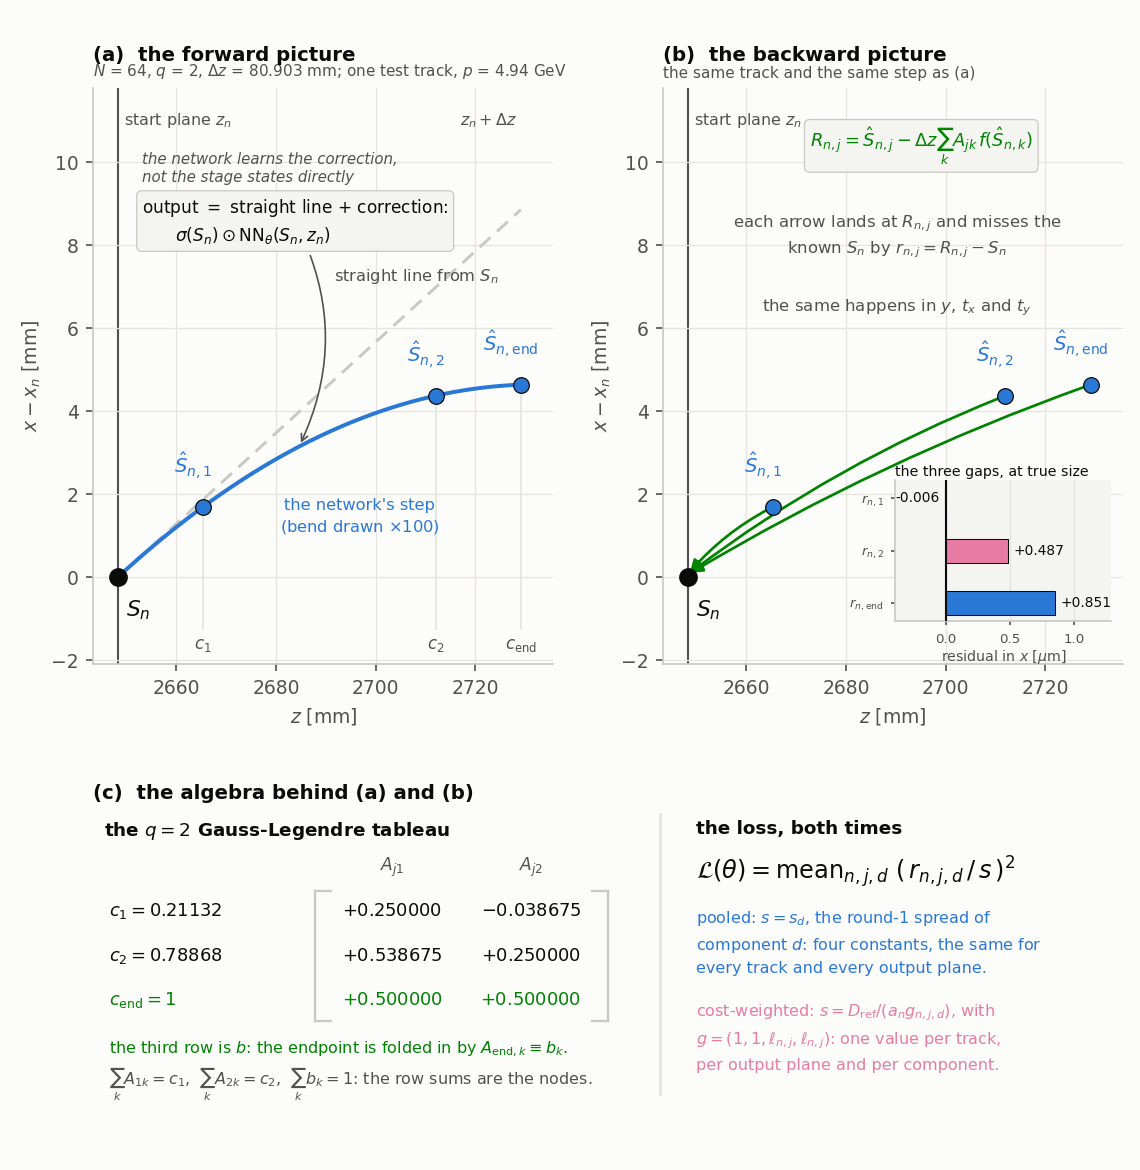
\includegraphics[width=0.9\linewidth]{fig_loss_schematic.png}
\caption{How one training step produces its residuals, drawn on the real
geometry of the $N = 64$, $q = 2$, $\Delta z = 80.903\mm$ network and on one
real test track of $4.94$ GeV. (a) The forward picture: the input state $S_n$
on the start plane $z_n$ (black dot), the straight line it would follow with no
field (dashed), and the network's three outputs at $z_n + c_j \Delta z$ for
$c_1 = 0.21132$, $c_2 = 0.78868$ and $c_{\mathrm{end}} = 1$, each of them the
straight line plus a correction $\sigma(S_n) \odot \mathrm{NN}_\theta$ as in
Eq.~\eqref{eq:netparam}, so that what the network learns is the correction to
the straight line, not the stage states directly. That correction is real but
small --- $42\um$ over an $80.9\mm$ step for this track --- so the bend is
drawn exaggerated by a factor of $100$; the straight line itself and the plane
positions are to scale. (b) The backward picture: from each output the
reconstruction of Eq.~\eqref{eq:recon-all} runs the step backwards to the start
plane, and each landing point misses the known $S_n$ by that output's
reconstruction residual. On the scale of the panel the three landings are
indistinguishable from $S_n$, so the inset draws the three gaps in $x$ at their
true size, in micrometres; $y$, $t_x$ and $t_y$ behave the same way. No
reference trajectory enters either panel: only the input, the tableau, and the
field at the network's own proposed positions. (c) The algebra behind both: the
$q = 2$ Gauss--Legendre tableau with its actual numbers and with the endpoint
row $A_{\mathrm{end},k} \equiv b_k$ appended, and the one-line form of the loss
with the two choices of divisor that separate Eq.~\eqref{eq:pooled-full} from
Eq.~\eqref{eq:cw-full}.
Source: \texttt{scripts/fig16\_loss\_schematic.py}.}
\label{fig:lossschematic}
\end{figure}

The loss the construction comes with treats every residual alike, once each
component has been put on a comparable footing. The state components have very
different units and sizes --- $x$ is hundreds of millimetres while $t_x$ is a
few tenths and dimensionless --- so squaring and summing them directly would
let $x$ dominate entirely. Each residual is therefore divided by a fixed scale
$s_d$ before squaring:
%
\begin{equation}
  \mathcal{L}_{\mathrm{pooled}}(\theta)
    = \operatorname*{mean}_{n,j,d}
      \left(\frac{r_{n,j,d}}{s_d}\right)^{\!2},
  \label{eq:pooled}
\end{equation}
%
where $n$ runs over the training states, $j$ over the $q+1$ outputs, $d$ over
the four predicted components, and $s_d$ is the \textbf{pooled} spread of
component $d$ over the training states, measured from the training population
itself and therefore label-free like everything else. This is the mean squared
normalised reconstruction residual, and it is what the first study and the
study immediately preceding this one both used.
Equation~\eqref{eq:pooled-full} at the head of this section is the same
expression written out, with the residual of Eq.~\eqref{eq:resid} substituted
and the sums over states, outputs and components shown explicitly.

Equation~\eqref{eq:pooled} asks for equal \emph{absolute} accuracy in every
component, on every track, at every plane --- and it gets it: the measured
per-step slope error is flat along the crossing. Two consequences follow, and
both were measured before any reweighted network was trained, by drawing
$8000$ (track, plane) states evenly over the $64$ start planes of a trained
$N = 64$, $q = 2$ network and asking what share of the loss each group of
states carries.

\paragraph{Consequence one: the loss is spent on the softest tracks.} A soft
track bends more, so its residuals are larger in absolute terms, so it takes
over an objective that counts absolute residuals. Of the pooled loss over those
$8000$ states, $89.8$ per cent comes from tracks of $3$--$8$ GeV, which are
$45.8$ per cent of the states; $8.8$ per cent comes from below $3$ GeV; and
$1.23$ per cent from the $10$--$50$ GeV window that the momentum region of
interest sits in, although that window holds $32.0$ per cent of the states.
The concentration is extreme even within that: the top one per cent of states
by contribution carry $98.3$ per cent of the whole loss.

\paragraph{Consequence two: the loss does not know where along the crossing it
is.} A slope residual and a position residual count the same in
Eq.~\eqref{eq:pooled}, although a slope error made on the first plane is
multiplied by more than five metres before the track reaches $z_1$ and a
position error is not. Measured the same way, the first quarter of the
crossing --- where an error has the longest lever arm and therefore costs the
most --- carries $0.65$ per cent of the loss, and the last quarter, where an
error costs least, carries $6.2$ per cent. The rank correlation between a
state's share of the loss and what that state's error actually costs at $z_1$
is $+0.68$ overall and $+0.53$ within the $10$--$50$ GeV window.

Neither distribution is something anyone asked for. They are what a pooled
normalisation produces, and together they set the question of this paper: if
the loss is asked for the right thing instead, how much of the endpoint error
goes away?

\subsection{The cost-weighted loss, derived}
\label{sec:theory-costweighted}

The replacement loss measures every residual as \textbf{the displacement it
would cause at the first SciFi plane, as a fraction of that track's own total
bend}, with the momentum region of interest weighted up. It changes the
weights inside the loss and nothing else: the same network code, the same
residuals of Eq.~\eqref{eq:resid}, the same tracks, the same optimiser.

\paragraph{The form.} Write the weighted loss as
%
\begin{equation}
  \mathcal{L}
    = \operatorname*{mean}_{n,j,d}
      \left(\frac{a_n\, e_{n,j,d}}{D_{\mathrm{ref}}}\right)^{\!2},
  \qquad
  \begin{aligned}
    e_{x} &= r_{x}, &\quad e_{y} &= r_{y},\\
    e_{t_x} &= r_{t_x}\,\ell_{n,j}, &\quad e_{t_y} &= r_{t_y}\,\ell_{n,j},
  \end{aligned}
  \label{eq:lossF}
\end{equation}
%
where every $e$ is now in millimetres; $\ell_{n,j}$ is the lever arm defined
below; $a_n$ is a factor that depends only on the track; and
$D_{\mathrm{ref}}$ is a fixed constant of the run that makes the whole
expression dimensionless. The two positions are weighted equally, in
millimetres, because the endpoint measure is radial; the separate $y$ scale of
Eq.~\eqref{eq:scale} stays where it belongs, in the network's output
parameterisation, and no longer doubles as a loss weight.
Equation~\eqref{eq:cw-full} in Section~\ref{sec:theory-pooled} writes this out
in full, with the residual substituted and the clamp on $a_n$ included.

\paragraph{The lever arm.}
%
\begin{equation}
  \ell_{n,j} = z_1 - \left(z_{\mathrm{start},n} + c_j \Delta z\right)
               + \Delta z,
  \label{eq:lever}
\end{equation}
%
where $z_{\mathrm{start},n}$ is the start plane of state $n$, $c_j \in [0,1]$
is the position of output $j$ inside the step (with $c_{q+1} = 1$ for the
endpoint), and $\Delta z$ is the step length. It is the distance that output
still has to travel before the track reaches $z_1$, \emph{plus one step}.
Multiplying a slope residual by it converts a slope into the millimetres of
displacement that slope will have produced by the time the track arrives, which
is what finally puts a slope residual and a position residual into the same
units so that they can be added.

The extra $\Delta z$ is \textbf{additive, not a floor}, and the choice matters.
Without it the lever arm would be exactly zero at the last plane of the
crossing, and the loss would place no weight at all on the final step --- which
is wrong, because an error made there still lands in the fit at full size as a
position error. A floor, $\max(z_1 - z, \Delta z)$, would fix the last plane
but leave every other plane untouched and introduce a kink. Adding one step
everywhere makes the last plane's weight small but finite and leaves every
other plane essentially unchanged, because $\Delta z$ is $1.6$ per cent of $L$
at $N = 64$ and less at the shorter steps. At $N = 64$ the lever arm runs from
$80.9\mm$ to $5258.7\mm$, a range of a factor $65$.

Figure~\ref{fig:lossweights} draws what that range does. Its first panel is the
lever arm seen geometrically, as the displacement a fixed slope error opens up
by the time the track reaches $z_1$; the remaining three are weight maps over
the plane $z$ and the momentum $p$, one for each loss, and they are the shortest
statement of what this section is about.

\begin{figure}[tbp]
\centering
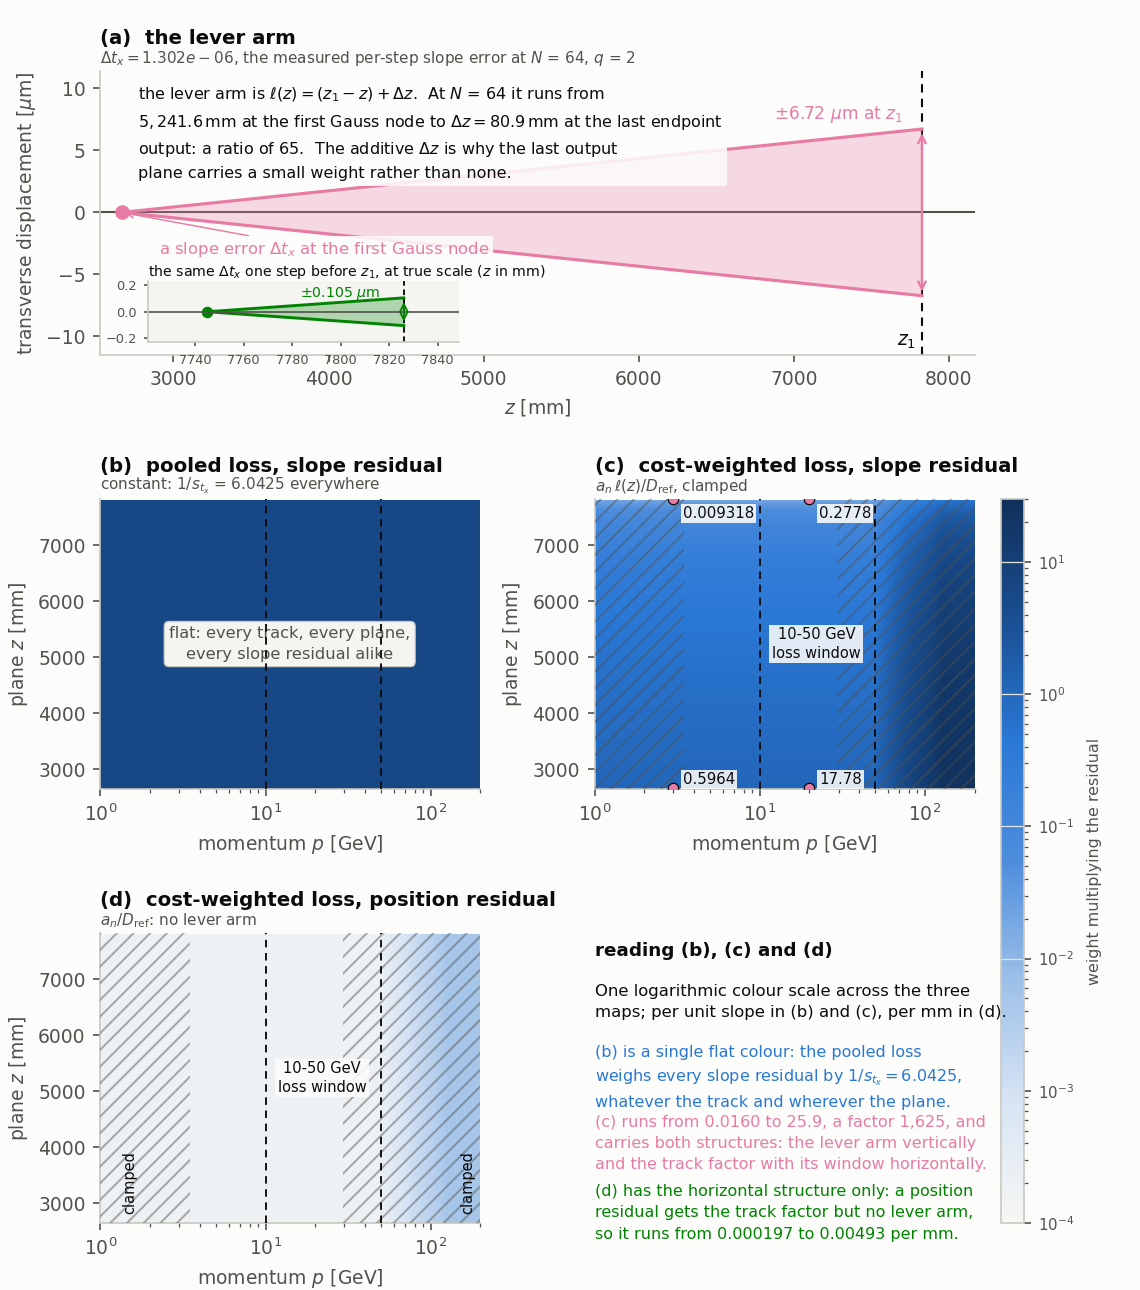
\includegraphics[width=0.9\linewidth]{fig_loss_weights_schematic.png}
\caption{What each loss does with the residuals, for the $N = 64$, $q = 2$
geometry. (a) The lever arm, geometrically: a slope error $\Delta t_x$ made at
the first Gauss node of the first step fans out into a displacement of
$\pm 6.72\um$ by the time the track reaches $z_1$, while the same error made
one step before $z_1$ fans into $\pm 0.105\um$, drawn at true scale in the
inset. Throughout the panel $\Delta t_x = 1.30 \times 10^{-6}$, the measured
per-step slope error of the pooled-loss network of this step length. The lever
arm of Eq.~\eqref{eq:lever} adds one step to that geometric distance, so it
runs from $5241.6\mm$ at the first Gauss node --- the largest lever arm the
loss actually weighs --- down to $\Delta z = 80.9\mm$ at the last endpoint
output, a ratio of $65$. The range quoted in the text above and in
Figure~\ref{fig:weights}, $80.9$ to $5258.7\mm$, is the weighting module's own
reported range, whose upper end is the value of Eq.~\eqref{eq:lever} at
$c = 0$, a plane on which no output sits; the two ends differ by $0.3$ per cent
and give the same factor $65$. (b) The pooled loss as a weight map over the
plane $z$ and the momentum $p$: one flat colour, the constant
$1/s_{t_x} = 6.0425$, on every track and at every plane. (c) The cost-weighted
loss on the same axes, $a_n\,\ell(z)/D_{\mathrm{ref}}$ with the clamp applied.
The hatched momenta are those at which the clamp binds, the dashed lines are
the $10$--$50$ GeV loss window, and the four marked points are the worked
example at the end of this section, annotated with its unclamped weights
$0.596$, $0.0093$, $17.8$ and $0.278$. (d) The same for a position residual,
$a_n/D_{\mathrm{ref}}$, which carries the track factor but no lever arm and so
has no vertical structure at all. Panels (b) to (d) share one logarithmic
colour scale, so the flat map and the $1625$-fold range of the drawn
cost-weighted map can be read against one another directly.
Source: \texttt{scripts/fig17\_loss\_weights\_schematic.py}.}
\label{fig:lossweights}
\end{figure}

\paragraph{The track factor.}
%
\begin{equation}
  a_n = \sqrt{W(p_n)}\;\frac{D_{\mathrm{ref}}}{D_n},
  \qquad
  D_n = \kappa\,\left|q/p\right|_n\,\bar{I}\,L,
  \label{eq:track}
\end{equation}
%
where $D_n$ is the track's \textbf{total transverse bend} across the whole
crossing; $\kappa = 10^{-3}$ is the unit conversion of
Eqs.~\eqref{eq:eom2}--\eqref{eq:eom3}; $\bar{I} = 3752.05$ T$\cdot$mm is the
field magnitude integrated along the $z$ axis over the crossing, evaluated once
with a $1024$-point midpoint rule and thereafter a pure constant;
$L = 5177.8\mm$; and $W(p)$ is the momentum window defined next.
$D_{\mathrm{ref}}$ is the median of $D_n$ over the run's first-round states,
$861.56\mm$ for the $N = 64$, $q = 2$ run. Dividing by $D_n$ converts an
absolute residual into a \emph{relative} one: an error of a given size counts
for more on a track that barely bends than on one that bends a great deal.
Since $D_n \propto 1/p$, that is precisely what removes the momentum skew of
Section~\ref{sec:theory-pooled}.

$D_n$ is deliberately the bend over the \emph{whole} crossing, a constant of
the track, and not the field integral of the particular step the residual sits
in. Dividing by the per-step integral would ask for constant relative accuracy
at every $z$, which in absolute terms would make the high-field middle of the
magnet worse --- and the middle is exactly where the bending happens.
$D_{\mathrm{ref}}$ is likewise fixed from the first round so that the objective
does not drift between rounds; it only sets the overall size of the loss, which
the trainer rescales anyway.

\paragraph{The momentum window.} $W(p)$ is a smooth top hat: equal to one on
$10$--$50$ GeV and falling off as a Gaussian in $\log p$ outside it, with a
floor,
%
\begin{equation}
  W(p) = \max\!\left(0.05,\;
    \exp\!\left[-\left(\frac{\log(p/p_{\mathrm{edge}})}{\log 2}\right)^{\!2}
    \right]\right),
  \label{eq:window}
\end{equation}
%
where $p_{\mathrm{edge}} = 10$ GeV below the band and $50$ GeV above it, and
$W = 1$ inside. The roll-off constant $\log 2$ means the window falls by a
factor $1/e$ one factor of two outside the band. It is a window and not a cut
because one network still has to work everywhere: $W$ is $0.05$ at $1$ and
$2$ GeV, $0.368$ at $5$ GeV, $1$ at $10$, $20$ and $50$ GeV, $0.368$ at
$100$ GeV and $0.05$ at $200$ GeV. The square root in Eq.~\eqref{eq:track} is
there because $a_n$ is squared inside Eq.~\eqref{eq:lossF}, so $\sqrt{W}$ makes
$W$ itself the multiplier on the squared residual. Throughout this paper
$10$--$50$ GeV is called the \textbf{loss window}, because that is what it is:
a parameter of the objective. It is not one of the paper's reporting bands,
which are $<3$, $3$--$8$, $8$--$20$, $20$--$50$ and $>50$ GeV; where the loss
window appears in a table it appears as an extra row and is labelled as such.

\paragraph{The clamp.} The factor $a_n$ scales as $|q/p|$, which spans about a
factor $200$ across this sample and $40\,000$ once squared. Left alone, the
handful of tracks above $100$ GeV would take a fifth of the loss. So $a_n$ is
clamped to $[1/5,\ 5]$ of its median over the round's own batch of training
states. The threshold moves slightly between rounds because the batch does;
$D_{\mathrm{ref}}$ does not. The factor five was chosen by a scan over the
clamp before any training, reported with the rest of the pre-flight in
Section~\ref{sec:results-weight}.

\paragraph{The loss is still label-free.} Both factors are functions of the
input state and the field map alone. $\ell_{n,j}$ is geometry: the start plane,
the nodes and the step length. $a_n$ needs $|q/p|$, which is the fifth
component of the input, and $\bar{I}$, which is an integral of the measured
map. Neither reads a reference trajectory, from an integrator or from a
simulation, so Eq.~\eqref{eq:lossF} preserves the property that makes the whole
construction worth having. That is not a detail: a weight built from the
reference error --- which would be the obvious way to weight by cost --- would
have made the objective as expensive to prepare as supervised training and as
fragile to a change of field map.

\paragraph{The reweighting must not move the minimum.} A weight changes how
much each residual counts. It must not change \emph{what a zero residual is},
or the network would be trained towards a different solution rather than
towards the same solution with a different emphasis. That is a checkable
statement and it was checked before any training: collocation states solved
exactly by a root-finder, with no network anywhere, give machine zero under
every weighting mode, between $6\times10^{-30}$ and $2\times10^{-29}$ of the
straight line's loss in the same units. The minimiser of
Eq.~\eqref{eq:lossF} is the minimiser of Eq.~\eqref{eq:pooled}; only the shape
of the surface around it differs.

\paragraph{Why not weight by the field.} The obvious alternative is to weight
up the strong-field region, on the grounds that that is where the bending
happens and therefore where the work is. It is wrong, and measurably so. Taking
the step-by-step error anatomy of a trained $N = 64$, $q = 2$ chain, over the
$64$ steps of the crossing, with the field magnitude on the axis running from
$0.221$ to $1.048$ T:

\begin{itemize}
  \item the per-step slope error against the field magnitude: Spearman $-0.575$,
  Pearson $-0.623$. The per-step error is \emph{worst where the field is
  weakest}, at the two low-field ends, not in the magnet's core;
  \item a step's cost at $z_1$ against the distance it still has to travel:
  Spearman $+0.996$, Pearson $+0.982$;
  \item a step's cost at $z_1$ against the field magnitude: Spearman $+0.124$,
  Pearson $-0.018$.
\end{itemize}

What a step's error costs at the far side follows the lever arm almost
perfectly and the field hardly at all. The lever arm is therefore the right
variable and the field is not, and the same measurement is the reason $D_n$
uses the bend over the whole crossing rather than the field integral of its own
step.

\paragraph{A worked example.} Take the $N = 64$, $q = 2$ run, where
$\Delta z = 80.90\mm$ and $D_{\mathrm{ref}} = 861.56\mm$, and compare a
$3$ GeV track with a $20$ GeV one. The $3$ GeV track has
$\qop = 0.0999$ and bends $D_n = 1941\mm$ across the crossing; it sits outside
the loss window, so $W = 0.05$, the floor, and
$a_n = \sqrt{0.05}\times 861.56/1941 = 0.0992$. The $20$ GeV track has
$\qop = 0.0150$ and bends $D_n = 291\mm$; it sits inside the window, so $W = 1$
and $a_n = 861.56/291 = 2.959$, a factor $29.8$ larger.

Now place each of them at a plane, and take the lever arm at the two ends of
the crossing in round terms, $\ell = L$ for an output near the start and
$\ell = \Delta z$ for the last output plane, whose ratio is exactly $N = 64$. A
slope residual on the $20$ GeV track near the start carries a weight
$a_n \ell / D_{\mathrm{ref}} = 17.8$ per unit of slope. The same residual on
the $3$ GeV track at the same place carries $0.596$ --- the factor $29.8$
again. The same residual on the $20$ GeV track at the \emph{last} plane carries
$0.278$, a factor $64$ down from the lever arm alone. And on the $3$ GeV track
at the last plane it carries $0.0093$. The extremes differ by a factor
$\mathbf{1908}$. A position residual, which has no lever arm, carries
$1.15\times10^{-4}$ per millimetre on the $3$ GeV track and
$3.43\times10^{-3}$ per millimetre on the $20$ GeV one. Under
Eq.~\eqref{eq:pooled} all four of those slope residuals would have counted the
same. These are the unclamped values; the clamp of $[1/5, 5]$ then trims the
tails of the $a_n$ distribution, which is why the realised spread is smaller
than $1908$ and why the clamp is a knob worth scanning.

Figure~\ref{fig:weights} shows the four factors of the weight separately.

\begin{figure}[tbp]
\centering
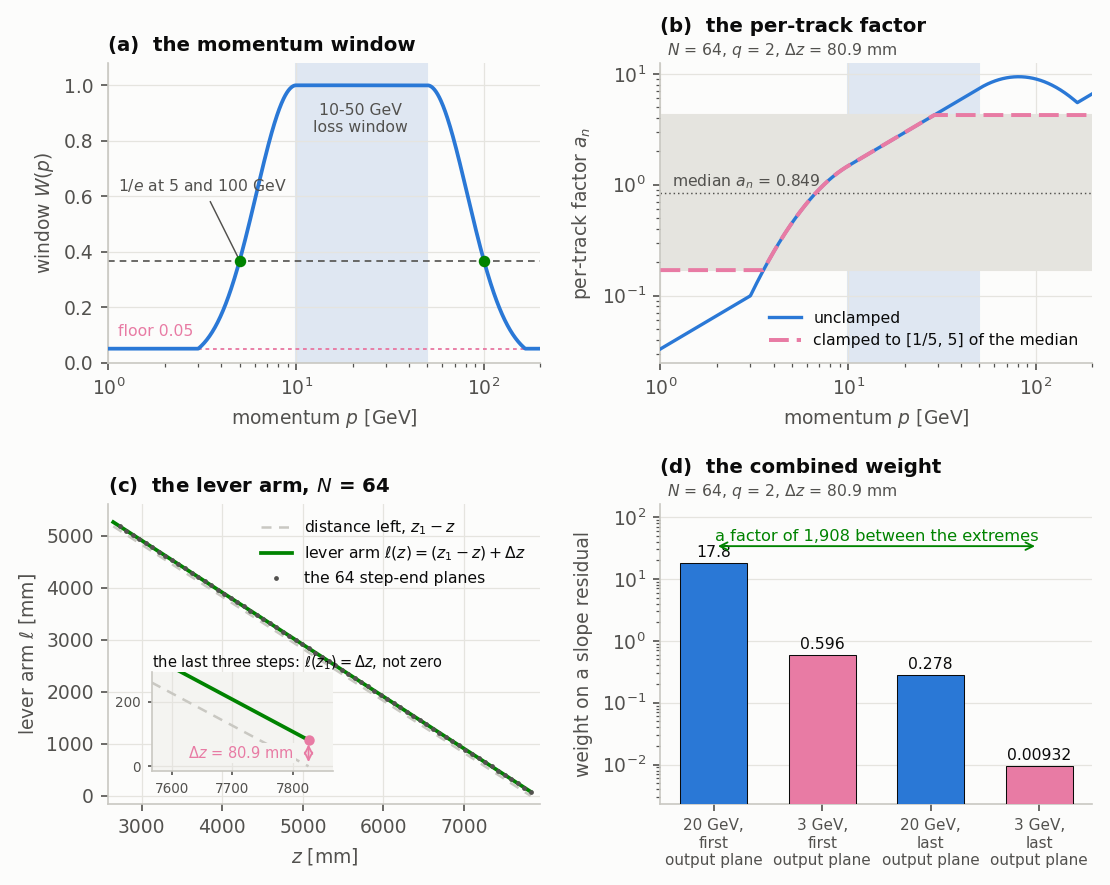
\includegraphics[width=0.9\linewidth]{fig_weights.png}
\caption{The four pieces of the cost-weighted loss of
Eq.~\eqref{eq:lossF}. (a) The momentum window $W(p)$ of
Eq.~\eqref{eq:window}: flat at one over the $10$--$50$ GeV loss window, falling
as a Gaussian in $\log p$ outside it and floored at $0.05$, so that no track is
ever ignored. (b) The track factor $a_n(p)$ of Eq.~\eqref{eq:track}, unclamped
and clamped to $[1/5, 5]$ of the batch median, showing which tracks the clamp
removes weight from at each end. (c) The lever arm $\ell(z)$ of
Eq.~\eqref{eq:lever} across the crossing for the $N = 64$, $q = 2$ network,
from $5258.7\mm$ at the start to $80.9\mm$ at the last output plane, with the
additive $\Delta z$ visible as the nonzero value at $z_1$. (d) The four weights
of the worked example --- a $3$ GeV and a $20$ GeV track, each at the first and
at the last output plane --- whose extremes differ by a factor $1908$.
Source: \texttt{scripts/fig07\_weights.py}, from the constants of the loss
module.}
\label{fig:weights}
\end{figure}

\subsection{The three reference points}
\label{sec:theory-references}

An error in micrometres means nothing on its own. Every number in this paper is
quoted against three fixed points, which answer three different questions and
must not be confused with one another. The numbers themselves are in
Section~\ref{sec:scheme}; what follows is what each one can and cannot say.

\begin{enumerate}
  \item \textbf{Exact collocation: the ceiling.} The same $q$-stage
  Gauss--Legendre equations, on the same states, at the same step length,
  chained the same $N$ times, solved directly by a root-finder in double
  precision with no network anywhere. Because the training loss is zero exactly
  when the network's outputs solve those equations, this is the best a network
  of that $(N, q)$ could possibly be: the answer the objective is pointing at.
  It says whether a given network is limited by its own optimisation or by the
  scheme it is solving. It says nothing about whether the scheme is the right
  scheme.
  \item \textbf{Sixth-order Runge--Kutta at $0.1\mm$: the reference.} Butcher's
  seven-stage explicit method of order six, integrating
  Eqs.~\eqref{eq:eom1}--\eqref{eq:eom4} through the same measured field map in
  $0.1\mm$ steps from the same starting state. Written RK6 throughout. Every
  error in this paper that is not explicitly against something else is against
  this: it is the same physics the network is trained on, integrated far more
  finely than the network's step. It says how well the network solves the
  problem it was given. It cannot say whether that problem is the particle's
  real trajectory, because it is a \emph{field-only} reference: it knows the
  magnetic field and nothing about the material the particle crosses.
  \item \textbf{The Geant4-true SciFi state: the truth.} The simulated
  particle's actual state on its own first SciFi plane, taken from the
  simulation that produced the sample, including multiple Coulomb scattering
  off the material in the way and any energy it lost there. Comparing the
  reference against this measures what the field-only description leaves out;
  the classical parameterisation of the scattering width is that of Lynch and
  Dahl~\citep{lynch1991}. This is the only one of the three that is a physical
  statement about a particle. It says what accuracy is worth chasing: driving a
  field-only surrogate far below the material term buys nothing in a fit that
  has to model the material anyway. It cannot be used to score the network
  directly, because the network was never trained on it and by construction
  cannot reproduce it.
\end{enumerate}

The ordering matters and is easy to get wrong. A network can be far above its
ceiling and still far below the material term, in which case the honest reading
is that the surrogate is limited by its optimiser but the limitation does not
yet matter physically. Section~\ref{sec:results-truth} makes that comparison
explicitly rather than leaving it to the reader.

\subsection{Metrics and the stopping rule}
\label{sec:theory-metrics}

Two different errors are reported throughout and they must be kept apart.

\begin{itemize}
  \item \textbf{Endpoint error.} The network is applied $N$ times, by the loop
  of Section~\ref{sec:theory-chaining}, starting from a test track's real state
  on the last Upstream Tracker plane, and its state on the first SciFi plane is
  compared with the RK6 reference carried to that same plane. This is the
  quantity the track fit would actually experience, and it contains every
  accumulation effect the chain produces.
  \item \textbf{Single-step error.} The network is applied \emph{once},
  starting from an RK6 reference state on some intermediate plane, and its
  output is compared with RK6 taken from that same state over that same step.
  This measures the network in isolation, with no accumulation whatever. Where
  a single-step number appears it is always said to be a single step; where it
  does not, the number is an endpoint.
\end{itemize}

The position error of a prediction is quoted in two ways. The
\textbf{radial} metric is $\sqrt{\Delta x^2 + \Delta y^2}$, and it is the
headline measure of this paper, because a track fit cares how far away the
prediction is and not in which direction. The \textbf{max metric} is
$\max(|\Delta x|, |\Delta y|)$, which is what the first study used and what
several of the stored result files carry, so it is reported wherever a
comparison with earlier work is being made. Slope errors are reported per
component and, as stated in Section~\ref{sec:intro-cost}, as dimensionless
numbers.

Over a set of tracks, five summaries are used.

\begin{itemize}
  \item The \textbf{median} of the absolute deviation, which is the headline
  for every table. It is used rather than the mean because the distribution has
  a long tail and a mean would report the tail rather than the typical track.
  \item The \textbf{95th percentile}, written p95, of the same distribution.
  This is where the tail shows, and a real-time system schedules against the
  tail rather than against the median.
  \item The \textbf{signed median}: the median of the signed deviation rather
  than of its magnitude. A signed median much smaller than the median magnitude
  means the typical track is missed in either direction, which is scatter; a
  signed median close to the median magnitude means the tracks are being bent
  systematically one way, which is a bias and a different problem.
  \item The \textbf{68 per cent half-width}: half the distance between the
  16th and 84th percentiles of the signed deviation. For a Gaussian it equals
  the standard deviation, but unlike the standard deviation it is not dragged
  by a few outliers.
  \item The \textbf{RMS}, the root mean square of the signed deviation, quoted
  beside the half-width wherever the two disagree, because the size of the
  disagreement is itself the statement about how heavy the tail is.
\end{itemize}

Two further quantities are used in the decomposition of
Section~\ref{sec:results-anatomy} and are defined here.

\textbf{Coherence} asks whether a chain's per-step errors add or cancel. For
one track, form the magnitude of the \emph{sum} of the per-step slope errors
along the chain and divide it by the sum of their magnitudes. If the $N$ steps
erred independently and at random, that ratio would be about $1/\sqrt{N}$; if
every step erred in the same direction it would be one. Quoting the measured
ratio beside its $1/\sqrt{N}$ reference says directly by what factor the steps
are more aligned than chance.

The \textbf{explained fraction} asks whether the endpoint error really is
accumulated slope error. Build a model of the endpoint error as the sum over
steps of each step's own position error plus that step's slope error multiplied
by the distance it still has to travel, and take the ratio of that model to the
measured endpoint error. A fraction near one means the decomposition is
complete and the endpoint error is exactly what the lever-arm picture says it
is; a fraction well below one means something else is happening.

\paragraph{Training, and the vocabulary of stopping.} The networks are trained
with L-BFGS, a quasi-Newton optimiser that builds an approximation to the
curvature of the loss surface from the last few gradient differences and takes
a step using it~\citep{liu1989}. It converges quickly to its own idea of a
minimum and then stops, so training does not proceed as one long descent but as
a sequence of fresh starts. Three terms follow from that and are used
throughout.

\begin{enumerate}
  \item A \textbf{restart} is one run of the optimiser, from the current
  weights, to its own convergence. Its curvature history is discarded at the
  start of each one.
  \item A \textbf{round} is $25$ consecutive restarts, after which a fresh
  batch of $32\,000$ collocation states is drawn and the network is scored on
  the validation tracks. The round is the unit in which progress is measured,
  because a single restart's validation number wanders by $10$ to $20$ per
  cent.
  \item The \textbf{validation headline} of a run is the median validation
  endpoint error of its last ten rounds, quoted with the round-to-round spread
  beside it. It is not the final checkpoint's number, which is one draw from
  that wandering.
\end{enumerate}

\paragraph{The plateau rule.} A run has \textbf{plateaued} once the median
validation error of its last ten rounds is no more than $5$ per cent below the
median of the ten rounds before it, and that holds at each of the last three
rounds. The rule was written into the folder specification before the runs were
submitted, and it was applied to the earlier pooled-loss runs' own logs as well
as to the new ones, so that neither side of the comparison could be favoured by
a rule chosen afterwards.

It is one-sided on purpose. An earlier two-sided version --- the last ten
rounds within $5$ per cent of the ten before, in either direction --- was tried
and discarded, because the round-to-round error wanders by $8$ to $23$ per cent
and ten-round medians therefore rarely land within $5$ per cent of each other
even long after a run has stopped improving. The question that matters for
stopping is not whether a run is steady but whether it is \emph{still getting
better}, so the rule fires only when the improvement has gone.

\paragraph{Convergence is never called from the loss.} This deserves its own
paragraph because ignoring it cost this programme a week of farm time and one
set of published numbers. The training loss and the held-out error are not the
same signal. Applying the rule above to the earlier pooled-loss runs' round
logs showed that \emph{none} of the sixteen had plateaued when training was
stopped by hand on the strength of a flat loss: every one of the eleven runs
with twenty or more rounds was still improving, by $5$ to $24$ per cent per ten
rounds. Eleven falls out of eleven has probability $0.0005$ if the round-to-
round movement were pure noise, so that is a trend and not scatter. Those runs'
numbers were therefore where training stopped, not where it converges, and
every one of them had to be extended to its own plateau before any comparison
could mean anything. All comparisons in Section~\ref{sec:results} use the
extended runs; the one table that uses the stopped snapshot says so in its
caption.

\paragraph{The pre-registered criterion.} For completeness, the criterion by
which the reweighting was to be judged was also fixed in advance, and it is the
one place in this paper where the loss window appears as a reporting band.
Success required the $N = 64$, $q = 2$ network's test radial error to clear the
$\pm 13$ per cent run-to-run band downward, \emph{and} its median per-step
slope error to fall below its then-current value of $1.6\times10^{-6}$, both
reported overall and in the $10$--$50$ GeV window. A partial result was defined
as an in-band improvement without an overall one, to be read as the window
having been made too hard, with the clamp as the knob. A null result was
defined as nothing clearing the band, to be read as the residual not being the
binding constraint. Section~\ref{sec:results-headline} reports the outcome
against that criterion and nothing else.


\section{Data and machinery}
\label{sec:data}

This section describes the material a chained network is trained on and scored
against, and the machinery that turns raw simulation into that material. I
begin with the simulated sample and where it came from
(Section~\ref{sec:data-sample}), then the piece of the detector the paper is
about, the magnet crossing, and the field that acts inside it
(Section~\ref{sec:data-crossing}). I then give the selection as a numbered
cascade with the row counts at every stage (Section~\ref{sec:data-cuts}), the
momentum spectrum and the five bands every table in this paper is reported in
(Section~\ref{sec:data-bands}), and the three checks the tracks had to pass
before any network saw them (Section~\ref{sec:data-gates}). Two short
subsections close the section: the units, stated once and properly, because the
slope convention in this paper differs from the labels on some of the files it
reads (Section~\ref{sec:data-units}); and the training protocol and its cost
(Section~\ref{sec:data-compute}). A reader who wants only the numbers can read
Tables~\ref{tab:cuts} to \ref{tab:materialfloor} and skip the prose.

\subsection{The sample}
\label{sec:data-sample}

Every track in this paper comes from official LHCb simulation. None of it was
generated here. That is a policy decision taken on 21 July 2026 and it has a
plain justification: a small configuration error in home-grown event generation
is easy to make and hard to see, whereas a centrally produced sample carries
validated conditions with it.

The sample is the LHCb \emph{TestFileDB} entry
\texttt{expected\_2024\_minbias\_xdigi}. TestFileDB is LHCb's registry of
reference data files: each entry names a set of files together with the exact
software conditions they were produced under, so that quoting the entry name
fixes the data and its provenance in one string. The entry points at production
\texttt{00212966}. Its files are in \textbf{XDIGI} format, the extended digitised
format, which holds the digitised detector banks \emph{and} the packed simulation
truth, so that for every simulated particle I can read both what the detector
would have recorded and what the particle actually did. The conditions are
detector description \texttt{dddb-20231017} and conditions tag
\texttt{sim-20231017-vc-mu100} for 2024 data taking. \textbf{DDDB} is the
detector description database, which says where every piece of the detector is
and what it is made of; \textbf{CondDB} is the conditions database, which says
what state the detector was in, including the magnet current and polarity. Five
of the entry's eight files, $19$ GB, are mirrored on the local CVMFS filesystem,
and $200$ events were read from them. No grid access was needed at any point.

The \texttt{mu100} in the conditions tag is the magnet polarity: it is the
\textbf{magnet-up} configuration, meaning the dipole's vertical field component
points upward and positive particles are deflected in the $-x$ direction. This
matters here for one reason, and I state it plainly because it is the kind of
detail that silently invalidates work.

\begin{quote}
\fbox{\parbox{0.94\linewidth}{\small \textbf{Polarity.} The cross-magnet labels
stored in the harvested training file were integrated with the \emph{magnet-down}
map, \texttt{field.v8r1.down.bin}, md5 \texttt{af284c69\dots58e}: that was the
default in force when the file was written, before the sample's own polarity was
established. The sample is a magnet-up sample. \textbf{Every track in this paper
is integrated on the magnet-up map}, \texttt{field.v8r1.up.bin}, md5
\texttt{9e49ddc4313b589f273540e7e0bb513b}, and \textbf{the stored labels are not
used anywhere}: I take from that file only the particles, their real states on
real detector planes and their momenta, all of which are field-free quantities,
and I regenerate every trajectory myself. The two maps are exact negatives of
one another, so the mistake would have been a sign error on the whole bend, of
order a metre for a soft track, not a subtle one.}}
\end{quote}

\subsection{The crossing and the field}
\label{sec:data-crossing}

The extrapolation step this paper is about is the crossing of the dipole magnet:
from the last plane of the Upstream Tracker, at $z_0 = 2648.2\mm$, to the first
plane of the scintillating-fibre tracker, at $z_1 = 7826.0\mm$. The span is
$L = z_1 - z_0 = 5177.8\mm$. It is the longest routine step in the track fit and
the only one in which the trajectory is strongly curved, so it is where a cheap
surrogate would be worth most and where it is hardest to build.

I store each track's state on $257$ planes,
\begin{equation}
  z_k \;=\; z_0 + k\,\frac{L}{256}, \qquad k = 0, 1, \dots, 256,
  \label{eq:planes}
\end{equation}
spaced $20.2258\mm$ apart. The number $256$ is chosen so that every step count
used in this paper divides it: a chain of $N$ steps starts its step $k$ on plane
index $k \cdot (256/N)$ and ends on plane $256$, so the same stored track serves
$N = 2$, $64$, $128$ and $256$ without interpolation. The corresponding step
lengths are $\Delta z = L/N = 2588.9$, $80.9031$, $40.4516$ and $20.2258\mm$.

The field is read from the canonical LHCb field map, version v8r1, magnet-up
polarity, file
\texttt{/cvmfs/lhcb.cern.ch/lib/lhcb/DBASE/FieldMap/v8r1/cdf/field.v8r1.up.bin},
md5 \texttt{9e49ddc4313b589f273540e7e0bb513b}. The map is a table of the three
field components on a regular Cartesian grid of $100\mm$ cells, and a field value
at an arbitrary point is obtained by \textbf{trilinear interpolation}: the value
is a weighted average of the eight corner values of the cell the point falls in,
linear in each coordinate. The consequence matters for everything in
Section~\ref{sec:scheme} and I flag it here. Trilinear interpolation is
continuous but its derivative is not: crossing a cell face, the field is
unchanged but its slope jumps. A crossing of the magnet passes about $52$ such
faces. The field a high-order integrator sees is therefore piecewise smooth with
kinks, which is written $C^0$, and not the smooth function such an integrator's
order was derived for.

On the beam axis the vertical component $B_y$ is $0.207$ T at $z_0$, rises to a
peak of $1.048$ T near $z = 4700\mm$, and has fallen back to $0.304$ T at
$z_1$.
Almost all of the deflection therefore happens in the middle third of the
crossing and almost none at either end, which is worth holding on to: a chain of
equal steps in $z$ is not a chain of equally difficult steps. A real $2.9$ GeV
track in this set is displaced $1204.8\mm$ in $x$ relative to where a straight
line would have taken it, and that displacement falls as the inverse of the
momentum, so a $45$ GeV track bends about fifteen times less over the same
distance. Figure~\ref{fig:crossing} draws these three things together: the
field on the beam axis, the plane grids of the three chains, and $x(z)$ for six
real test tracks.

\begin{figure}[tbp]
  \centering
  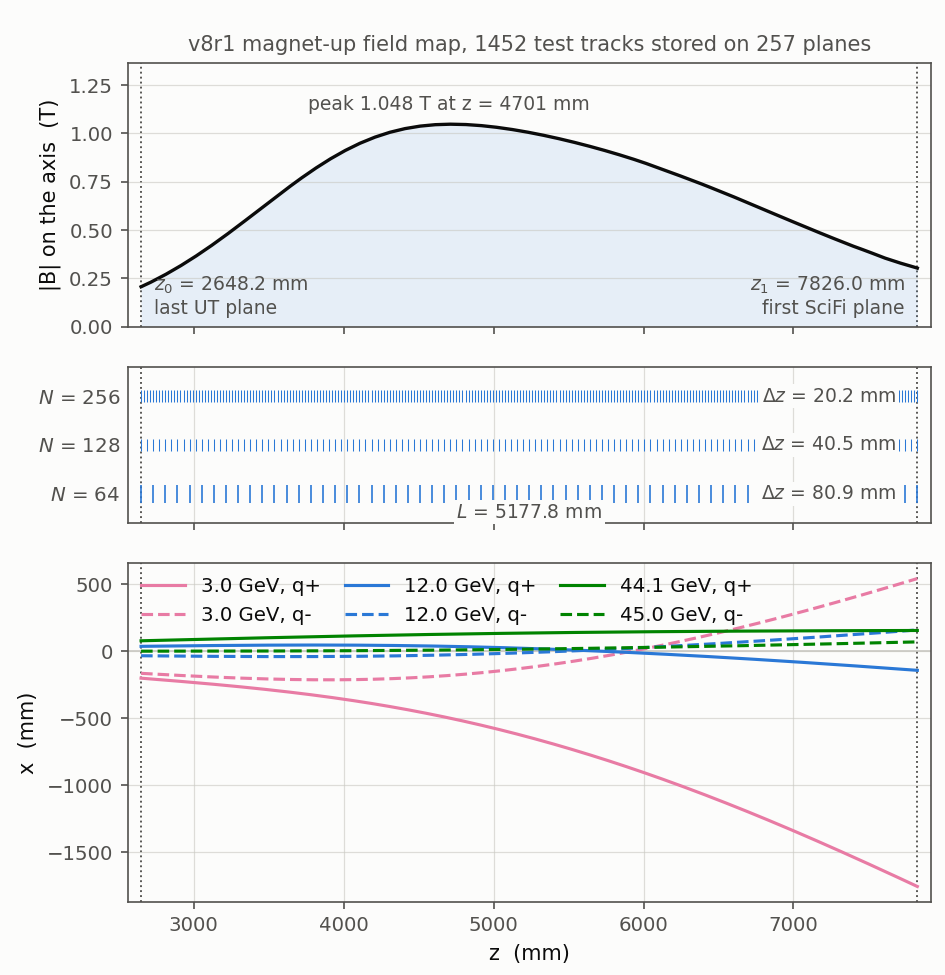
\includegraphics[width=0.9\linewidth]{fig_crossing.png}
  \caption{The magnet crossing this paper is about, in three registers. Top:
  the field magnitude on the beam axis ($x = y = 0$) between
  $z_0 = 2648.2\mm$ and $z_1 = 7826.0\mm$, read from the v8r1 magnet-up map:
  $0.207$ T at the entry plane, a peak of $1.048$ T near $z = 4700\mm$, and
  $0.304$ T at the exit plane, so almost all of the deflection happens in the
  middle third. Middle: the plane grids of the three
  chains used in this paper, $N = 64$, $128$ and $256$, drawn as ticks at
  $z_0 + k\,\Delta z$ with $\Delta z$ labelled; the $N = 256$ grid is the
  $257$-plane grid every stored trajectory lives on. Bottom: $x(z)$ for six
  real test tracks, the nearest track to $3$, $12$ and $45$ GeV in each charge,
  taken from the stored sixth-order trajectories and drawn to scale in
  millimetres. The $1/p$ bend is the whole reason a single step across the
  magnet cannot work.
  Source: \texttt{scripts/fig01\_crossing.py}, \texttt{results/fig01\_crossing.csv}.}
  \label{fig:crossing}
\end{figure}

\subsection{The cut cascade and the split}
\label{sec:data-cuts}

The tracks are built from the harvested simulation in nine selection steps
followed by one fiducial requirement. I give them as a protocol, with the row
counts after each step in Table~\ref{tab:cuts}.

\begin{enumerate}\setlength{\itemsep}{2pt}
  \item Take every cross-magnet row in the harvested set, both directions of
  travel. A \emph{row} here is one pair of planes to be extrapolated between,
  for one particle.
  \item Require that the plane before the magnet really is an Upstream Tracker
  plane, that is $z_{\mathrm{pre}} > 1500\mm$. Below that the particle had no
  hit in the Upstream Tracker at all and the row would start on a vertex-detector
  plane, which is a different and much longer extrapolation. This removes
  $2476$ rows.
  \item Require that both directions survived for the particle, since the
  forward and backward legs are built as a matched pair and I do not want a
  half-pair in the set. This removes $2388$ rows.
  \item Require $2 < \eta < 5$, where the \textbf{pseudorapidity}
  $\eta = -\ln\tan(\theta/2)$ is a dimensionless measure of how forward a
  particle goes, with $\theta$ the angle to the beam axis; $\eta = 2$ is about
  $15.4^\circ$ from the beam and $\eta = 5$ about $0.8^\circ$. This window is
  LHCb's nominal acceptance. It is evaluated on the truth pseudorapidity at the
  particle's origin and removes $1240$ rows.
  \item Require $1 < p < 200$ GeV. This is already the harvested set's own
  domain cut, so it removes nothing here, and I list it so that the domain is
  on the record.
  \item Require that the particle is not an electron, $|\mathrm{PID}| \neq 11$.
  Electrons radiate in material and their trajectories are not describable by an
  equation of motion that conserves momentum. This removes $4780$ rows, the
  largest single cut.
  \item Re-check that both directions are still present after the cuts. Nothing
  is removed.
  \item Keep the forward row only, one row per particle.
  \item Require that the row's own planes sit within $60\mm$ of the nominal
  $z_0$ and $z_1$, so that every track in the set really is crossing the same
  gap. In the surviving set $z_{\mathrm{pre}}$ runs from $2593.2$ to
  $2663.3\mm$ and $z_{\mathrm{post}}$ from $7818.7$ to $7833.5\mm$. This removes
  $775$ particles and leaves $\mathbf{14{,}482}$ crossings.
  \item \textbf{Fiducial.} A track is \emph{fiducial} if it stays inside the
  region the field map covers for its whole path: I require $x$ and $y$ to lie
  inside the map at all $257$ stored planes and every stored number to be
  finite. On the magnet-up polarity, which is the sample's own, this removes
  nothing. It is not a formality: on the reversed polarity soft backward legs
  bend out to the edge of the map, where the loader clamps the field and the
  trajectory stops meaning anything.
\end{enumerate}

\begin{table}[tbp]
  \centering
  \caption{The cut cascade that produced the track set. A row is one plane pair
  for one particle; the particle column counts distinct particles surviving.
  The last two lines are the two requirements that define the set used
  throughout this paper: a common crossing and a fiducial trajectory.
  Source: \texttt{results/tab\_dataset\_cuts.csv}.}
  \label{tab:cuts}
  \small
  \setlength{\tabcolsep}{4pt}
  \begin{tabular}{rp{6.0cm}rrrr}
    \toprule
    & requirement & rows in & removed & rows out & particles \\
    \midrule
    1 & cross-magnet rows, both directions & $41{,}398$ & $0$ & $41{,}398$ & $21{,}932$ \\
    2 & the pre-magnet plane is an Upstream Tracker plane & $41{,}398$ & $2476$ & $38{,}922$ & $20{,}655$ \\
    3 & both directions kept for the particle & $38{,}922$ & $2388$ & $36{,}534$ & $18{,}267$ \\
    4 & $2 < \eta < 5$ & $36{,}534$ & $1240$ & $35{,}294$ & $17{,}647$ \\
    5 & $1 < p < 200$ GeV & $35{,}294$ & $0$ & $35{,}294$ & $17{,}647$ \\
    6 & not an electron & $35{,}294$ & $4780$ & $30{,}514$ & $15{,}257$ \\
    7 & both directions still present & $30{,}514$ & $0$ & $30{,}514$ & $15{,}257$ \\
    8 & forward row only & $30{,}514$ & $15{,}257$ & $15{,}257$ & $15{,}257$ \\
    9 & planes within $60\mm$ of $z_0$ and $z_1$ & $15{,}257$ & $775$ & $\mathbf{14{,}482}$ & $\mathbf{14{,}482}$ \\
    10 & fiducial: inside the map at all $257$ planes & $14{,}482$ & $0$ & $\mathbf{14{,}482}$ & $\mathbf{14{,}482}$ \\
    \bottomrule
  \end{tabular}
\end{table}

The $14{,}482$ crossings are split \textbf{by particle}, inherited from the
harvested set with seed $20260718$: $11{,}567$ training, $1463$ validation and
$1452$ test. Splitting by particle rather than by row matters because the rows
of one particle are strongly correlated; splitting by row would leak information
from training into test. The validation split is used for the stopping rule and
the test split is used for every number reported as a result.

\subsection{The momentum spectrum and the five bands}
\label{sec:data-bands}

Everything in this paper that varies with momentum is reported in five bands,
$<3$, $3$--$8$, $8$--$20$, $20$--$50$ and $>50$ GeV, with the band population
always shown. Where a loss or a design choice singles out the $10$--$50$ GeV
window I report that window as an extra row, labelled
``$10$--$50$ (loss window)''; it deliberately overlaps two of the five bands and
is not part of the partition. Band membership is taken from each track's own
momentum, not from any stored band index.

\begin{table}[tbp]
  \centering
  \caption{The three splits in the paper's five momentum bands, with the
  $10$--$50$ GeV loss window reported alongside. The window overlaps the
  $8$--$20$ and $20$--$50$ bands on purpose and is not part of the partition, so
  its count is not added into the split total. The $>50$ GeV band is thin
  everywhere and holds \textbf{30 test tracks}; every statement made about it in
  this paper is read with that in mind.
  Source: \texttt{results/tab\_dataset\_bands.csv}.}
  \label{tab:splitbands}
  \small
  \setlength{\tabcolsep}{5pt}
  \begin{tabular}{lrrrrrr}
    \toprule
    & \multicolumn{2}{c}{train ($11{,}567$)} & \multicolumn{2}{c}{validation ($1463$)} & \multicolumn{2}{c}{test ($1452$)} \\
    \cmidrule(lr){2-3}\cmidrule(lr){4-5}\cmidrule(lr){6-7}
    band [GeV] & $n$ & median $p$ & $n$ & median $p$ & $n$ & median $p$ \\
    \midrule
    $<3$        & $1339$ & $2.62$  & $181$ & $2.63$  & $164$ & $2.63$  \\
    $3$--$8$    & $5283$ & $4.83$  & $668$ & $4.89$  & $655$ & $4.94$  \\
    $8$--$20$   & $3391$ & $11.91$ & $441$ & $11.82$ & $433$ & $12.48$ \\
    $20$--$50$  & $1326$ & $27.34$ & $154$ & $27.97$ & $170$ & $26.88$ \\
    $>50$       & $228$  & $65.34$ & $19$  & $61.04$ & $30$  & $70.64$ \\
    \midrule
    $10$--$50$ (loss window) & $3756$ & $16.50$ & $470$ & $15.85$ & $487$ & $16.18$ \\
    \bottomrule
  \end{tabular}
\end{table}

Table~\ref{tab:splitbands} gives the populations. The three splits carry the
same spectrum: median momentum $6.75$, $6.78$ and $6.86$ GeV in train,
validation and test, and band fractions that agree to about one percentage point
in every band. The set is dominated by soft tracks, as a minimum-bias sample
must be: $56$ to $58$ per cent of every split sits below $8$ GeV and the
$20$--$50$ GeV band holds about $11$ per cent. The extremes are $1.50$ and $178.6$ GeV in
training, and $1.73$ and $143.4$ GeV in test. The
pseudorapidity fills the selection window, $2.00$ to $5.00$, with a median of
$3.49$ in training and $3.53$ in test.

Two further properties of the population are used later. The charge is close to
balanced, $51.2$ per cent positive in training and $50.9$ per cent in test,
which is what lets Section~\ref{sec:scheme-fieldonly} separate a
charge-antisymmetric systematic from a charge-blind width by splitting the set
in two. And the particle composition is dominated by pions: in the test split,
$1120$ pions ($77.1$ per cent), $163$ kaons ($11.2$), $152$ protons ($10.5$) and
$17$ muons ($1.2$); the training split is the same to within a percentage point.
Electrons are absent by construction. Figure~\ref{fig:sample} shows the sample
in four registers: the momentum spectrum of the three splits with the band edges
drawn, the composition and charge balance of the test split, the starting
footprint of the test tracks on the plane $z_0$, and the pseudorapidity
distribution.

\begin{figure}[tbp]
  \centering
  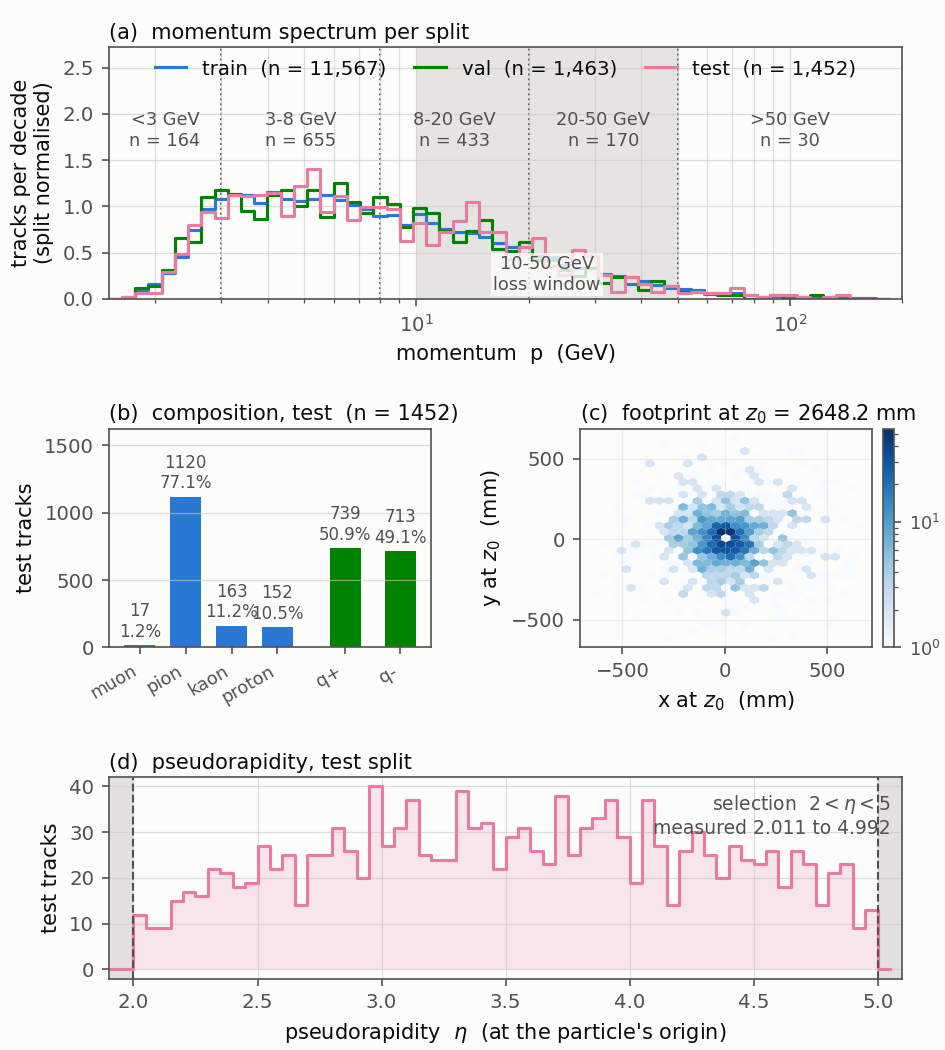
\includegraphics[width=0.9\linewidth]{fig_sample.png}
  \caption{What the track sample is made of. Panel (a): the momentum spectrum
  of the three splits, each normalised so that the shapes can be compared, on a
  logarithmic axis from $1.5$ to $200$ GeV, with the four interior band edges
  drawn, each band labelled with its test-split count, and the $10$--$50$ GeV
  loss window shaded. Panel (b): the composition of the test split, the four
  particle types that survive the non-electron cut ($1120$ pions, $163$ kaons,
  $152$ protons, $17$ muons) and the charge balance ($50.9$ per cent positive),
  with counts and percentages printed on the bars. Panel (c): the starting
  footprint of the test tracks, $(x, y)$ on the plane $z_0 = 2648.2\mm$, as a
  hexagonal-bin density on a logarithmic colour scale. Panel (d): the
  pseudorapidity distribution of the test split with the $2 < \eta < 5$
  selection drawn. Every count on the figure is asserted against
  \texttt{results/paper\_numbers.json} before the figure is drawn.
  Source: \texttt{scripts/fig02\_sample.py}, \texttt{results/fig02\_sample.csv}.}
  \label{fig:sample}
\end{figure}

\subsection{The gates on the tracks}
\label{sec:data-gates}

Three checks stand between the raw selection and any use of these tracks. I
call them gates, and all three pass.

\paragraph{Gate 1: the track set reproduces its predecessor bit for bit.} The
same particles, selected the same way, were used in the preceding study of this
programme, on a coarser plane grid of $129$ planes. The new file is required to
carry the same validation and test particles, in the same order, with bit
identical start states, real detector states, planes, momenta and charges, and
to agree with the old trajectories on the $129$ shared planes. It does. The
largest position disagreement anywhere is
$\mathbf{1.5 \times 10^{-4}\,\mu\mathrm{m}}$; the largest slope disagreement is
$\mathbf{6.3 \times 10^{-11}}$, dimensionless (the gate file records it as
$6.3 \times 10^{-8}$ in its own units of slope $\times\,10^{3}$, and I convert);
and $q/p$ agrees exactly. Those residuals are not zero for a reason worth
stating: the integrator restarts its $0.1\mm$ steps at every stored plane, and
the new file stores twice as many planes, so the same trajectory is cut into
twice as many pieces and the last, shortened step of each piece falls
differently. A tenth of a nanometre is the size of that effect.

\paragraph{Gate 2: fiducial.} Every one of the $14{,}482$ trajectories stays
inside the field map at all $257$ planes, with every stored number finite. This
is step $10$ of the cascade and it removes nothing on this polarity, which is
itself the evidence that the polarity is right.

\paragraph{Gate 3: the reference closes.} The reference integrator is required
to undo itself: integrate a state forward across the magnet and back again, and
compare with where it started. Over $200$ momentum-stratified legs the round
trip closes to a median of $3.7 \times 10^{-6}\um$ and a worst case of
$4.4 \times 10^{-5}\um$ on the real map at a $0.1\mm$ step. This is not a test of
accuracy, because both halves carry the same truncation error, but it is a floor:
nothing built on this reference can be trusted below the level at which it fails
to undo itself. Section~\ref{sec:scheme-sixthorder} measures the reference
properly.

\paragraph{What no gate can remove.} The reference integrates the equation of
motion in the magnetic field and nothing else, while the simulated particle also
scatters off material and loses energy. The distance between the two is the
\textbf{material floor}: the gap between the particle's own real state on its
first fibre-tracker plane and the field-only trajectory carried to that same
plane. Table~\ref{tab:materialfloor} gives it in the paper's bands. It is
$1736\um$ in the median over the whole set and $8683\um$ below $3$ GeV. It is
not an error in the tracks and no better integrator and no better network can
reduce it. Section~\ref{sec:scheme-fieldonly} takes it apart into its physical
pieces and says which pieces are fixable.

\begin{table}[tbp]
  \centering
  \caption{The material floor: the particle's real simulated state on its own
  first fibre-tracker plane, minus the field-only sixth-order trajectory carried
  to that same plane, over all three splits concatenated ($14{,}482$ crossings).
  Positions are the max metric $\max(|\Delta x|, |\Delta y|)$ in micrometres;
  the slope column is the median of $\max(|\Delta t_x|, |\Delta t_y|)$ and is
  dimensionless. The last column is the fraction of tracks missing by more than
  one millimetre. The $10$--$50$ GeV row overlaps two bands and is not part of
  the partition. Source: \texttt{results/tab\_material\_floor.csv}.}
  \label{tab:materialfloor}
  \small
  \setlength{\tabcolsep}{5pt}
  \begin{tabular}{lrrrrr}
    \toprule
    band [GeV] & $n$ & median [\um] & p95 [\um] & median slope & $>1\mm$ \\
    \midrule
    all         & $14{,}482$ & $1736$ & $12{,}628$ & $4.94 \times 10^{-4}$ & $64.6\%$ \\
    $<3$        & $1684$     & $8683$ & $24{,}293$ & $3.34 \times 10^{-3}$ & $98.8\%$ \\
    $3$--$8$    & $6606$     & $2806$ & $10{,}849$ & $8.81 \times 10^{-4}$ & $87.9\%$ \\
    $8$--$20$   & $4265$     & $793$  & $4059$     & $2.17 \times 10^{-4}$ & $38.5\%$ \\
    $20$--$50$  & $1650$     & $324$  & $2048$     & $9.36 \times 10^{-5}$ & $13.9\%$ \\
    $>50$       & $277$      & $153$  & $850$      & $4.06 \times 10^{-5}$ & $4.7\%$  \\
    \midrule
    $10$--$50$ (loss window) & $4713$ & $532$ & $2973$ & $1.45 \times 10^{-4}$ & $25.1\%$ \\
    \bottomrule
  \end{tabular}
\end{table}

\subsection{Units}
\label{sec:data-units}

This subsection is short and it is binding on everything that follows.

\textbf{Slopes are dimensionless.} A track state is
$(x, y, t_x, t_y, q/p)$, and the two slopes are
\begin{equation}
  t_x = \frac{dx}{dz}, \qquad t_y = \frac{dy}{dz},
\end{equation}
built from a simulated hit's exit minus entry displacement divided by that
hit's own $\Delta z$. No arctangent is applied anywhere in the chain from the
simulation to these pages, so $t_x$ is a ratio of two lengths and not an angle.
I quote slopes and slope errors as dimensionless numbers in scientific
notation. I never write ``mrad'' and I never scale a slope by $10^{3}$.

This differs from the labels on some of the files this paper reads. Several
earlier result files in this programme write ``mrad'' for a slope difference
multiplied by $10^{3}$, which is not the same quantity as a milliradian. The
relation between the two is
\begin{equation}
  \Delta\theta \;\approx\; \frac{\Delta t_x}{1 + t_x^{2}},
\end{equation}
where $\theta = \arctan t_x$ is the true angle. Inside the acceptance,
$2 < \eta < 5$ gives $|t_x| \lesssim 0.27$, so the two agree to within $7$ per
cent at the very edge of the acceptance and within $1$ per cent for most tracks.
Whenever this paper reads a file whose slope column is scaled that way, the
scaling is divided out and the label discarded; the figure and table generators
do this at the point of reading, so no scaled slope reaches a table.

\textbf{Positions} are quoted in micrometres (\um) for errors and millimetres
(\mm) for geometry, and I say which. \textbf{Radial} error means
$\sqrt{\Delta x^{2} + \Delta y^{2}}$ and \textbf{max metric} means
$\max(|\Delta x|, |\Delta y|)$; the max metric is the more conservative of the
two and is never larger than the radial value. The metric is named beside every
number in this paper. Finally, I distinguish \textbf{endpoint error}, the
network applied $N$ times in succession from the particle's real Upstream
Tracker state and compared at the far end, from \textbf{single-step error}, one
application of the network from a state taken off the reference trajectory.
These differ by more than two orders of magnitude and I say which one every
number is.

\subsection{Compute and the training protocol}
\label{sec:data-compute}

Table~\ref{tab:fixed} lists what is held fixed across every run in this paper.
The point of fixing them is that a difference between two runs is then a
difference in the loss and in nothing else.

\begin{table}[tbp]
  \centering
  \caption{What is held fixed across every training run in this paper. The
  parameter count depends on the stage count $q$ because the network's output
  layer carries $q$ stage states and one end state; the three step counts used
  for the headline comparison have $18{,}956$, $22{,}052$ and $26{,}180$
  parameters at $q = 2$, $8$ and $16$.
  Source: \texttt{results/tab\_compute.csv}, \texttt{results/paper\_numbers.json}
  (\texttt{compute}), and
  \texttt{single\_network\_chain\_discrete\_approach/}\allowbreak\texttt{Block\_F\_reweighted\_loss/F4\_Writeup/page.md}.}
  \label{tab:fixed}
  \small
  \setlength{\tabcolsep}{5pt}
  \begin{tabular}{lp{9.4cm}}
    \toprule
    held fixed & value \\
    \midrule
    tracks & $14{,}482$ crossings from the official simulated sample, split by
      particle into $11{,}567$ train, $1463$ validation, $1452$ test \\
    network & two hidden layers of $128$ units, $\tanh$ activation; the module is
      \emph{imported} from the shared package rather than copied, so it cannot
      drift between runs \\
    seed & $0$, the same one for every run \\
    optimiser & L-BFGS, $200$ iterations per restart, history $120$, strong
      Wolfe line search; $25$ restarts per round \\
    states per round & $32{,}000$ collocation states, redrawn every round \\
    field map & v8r1, magnet up, md5 \texttt{9e49ddc4\dots513b} \\
    reference & seven-stage, sixth-order Runge--Kutta at a $0.1\mm$ step, from
      the same start state \\
    \bottomrule
  \end{tabular}
\end{table}

The optimiser is \textbf{L-BFGS} \citep{liu1989}, the limited-memory
Broyden--Fletcher--Goldfarb--Shanno method: a quasi-Newton method that builds an
implicit approximation to the inverse Hessian from the last few dozen gradient
differences rather than storing a full matrix, and takes a line-searched step
along the resulting direction. It is a deterministic full-batch method, which is
why the training protocol is organised in \textbf{restarts} rather than epochs:
one restart is $200$ L-BFGS iterations from the current parameters with a fresh
optimiser state, and restarting periodically is what lets the method escape the
flat regions where its curvature estimate has gone stale. Restarts are grouped
into \textbf{rounds} of $25$. At the start of every round a fresh set of
$32{,}000$ (track, plane) states is drawn, the same number from every plane, so
that no network can overfit a fixed draw; the loss is rescaled to $1$ at the
start of each round and again whenever it has fallen tenfold, each time with a
fresh optimiser, so that the line search always works on numbers of order one.

All training ran on the Nikhef HTCondor farm, one job per run, single-threaded
and in double precision. Single-threaded is not a preference: multithreaded
PyTorch spin-waits on these nodes and is dramatically slower. The median wall
time per restart, over the de-duplicated training history of each run, is
$77.2$ s for the $80.9\mm$-step network under the pooled loss and $77.7$ s under
the cost-weighted loss; $117.9$ and $118.3$ s for the $40.5\mm$-step network;
and $219.8$ and $184.1$ s for the $20.2\mm$-step network. Each restart runs its
full $200$ iterations; none of the six runs stopped early.

One trainer produced both losses. The cost-weighted trainer is the pooled-loss
trainer with the loss function swapped and a mode flag that restores the old
weights, and it is required to reproduce the old training \emph{bit for bit} in
that mode. It does: over three restarts on the same seed and the same states,
the two trainers give identical losses to the last digit, $1.0011 \times
10^{-4}$, then $8.6855 \times 10^{-8}$, $3.2594 \times 10^{-8}$ and
$1.9375 \times 10^{-8}$. That gate is what licenses every comparison in
Section~\ref{sec:results} to be read as a comparison of two losses rather than
of two pieces of software.

% ===========================================================================
\section{The scheme, measured on its own}
\label{sec:scheme}

Before any network appears, three things have to be measured. The first is the
integration scheme the network is being asked to satisfy: its coefficients are
constructed rather than copied, and a constructed tableau is worth nothing until
it has been checked on the machine that will use it
(Section~\ref{sec:scheme-tableau}). The second is how well that scheme does when
it is solved \emph{exactly}, with no network in it, and chained across the
magnet. Because the training loss is zero precisely when the network solves
those same equations, the exact solution is the \textbf{ceiling}: no network of
that step count and stage count can do better, and a network's score only means
something beside it (Section~\ref{sec:scheme-ceiling}). The third is the
reference the whole programme is scored against, a sixth-order Runge--Kutta
integration at a $0.1\mm$ step, whose own accuracy I measure rather than assume
(Section~\ref{sec:scheme-sixthorder}). Section~\ref{sec:scheme-fieldonly} then
asks the question behind all three: the reference solves its equation, but is
the equation what the simulated particle did? The answer sets the ceiling of the
programme as a whole, and it does not enter any network number in this paper.

\subsection{The tableau}
\label{sec:scheme-tableau}

Section~\ref{sec:theory-collocation} defined the tableau $(c, A, b)$ of a
$q$-stage Gauss--Legendre scheme and said that it is built here rather than
looked up. This subsection reports the construction and the battery of
identities that checks it, because a constructed tableau is worth nothing until
it has been checked on the machine that will use it.

The construction is three lines, and it is problem-independent:
\begin{enumerate}\setlength{\itemsep}{2pt}
  \item take the $q$-point Gauss--Legendre nodes and weights on $[-1, 1]$ from
  the standard Legendre routine, and map them affinely onto $[0, 1]$:
  $c = (x+1)/2$ and $b = w/2$;
  \item form the Lagrange basis polynomials $\ell_k$ on those nodes, written in
  \textbf{barycentric} form, $\ell_k(x) \propto w_k/(x - c_k)$ normalised to sum
  to one, which is numerically well conditioned where a Vandermonde solve would
  not be;
  \item set $a_{jk} = \int_{0}^{c_j} \ell_k(s)\,ds$, the collocation integrals,
  each evaluated with the same Gauss rule rescaled onto $[0, c_j]$, which is
  exact because $\ell_k$ has degree $q - 1$.
\end{enumerate}

Five identities then have to hold, and each one catches a different mistake.
\begin{enumerate}\setlength{\itemsep}{2pt}
  \item \textbf{Row sums.} $\sum_k a_{jk} = c_j$: a stage really sits at that
  fraction of the step. A transposed or mis-ordered $A$ fails here.
  \item \textbf{Quadrature.} $\sum_j b_j c_j^{m-1} = 1/m$ for $m = 1, \dots, 2q$:
  the rule integrates every polynomial up to degree $2q - 1$ exactly, which is
  the property that gives the method its order $2q$.
  \item \textbf{Collocation.} $A c^{m-1} = c^{m}/m$ for $m = 1, \dots, q$: the
  stage matrix really is the integral of the interpolating polynomial. A wrong
  node vector fails here even when the weights are right.
  \item \textbf{Symplecticity.} $b_j a_{jk} + b_k a_{kj} = b_j b_k$, an exact
  property of Gauss methods \citep{hairer2006} that the construction never
  imposes. Finding it satisfied to roundoff is an independent check that these
  are the Gauss coefficients and not merely a consistent tableau.
  \item \textbf{Literature.} For $q = 1$, $2$ and $3$, comparison element by
  element with the closed-form tableaus of Hairer and Wanner
  \citep[table~IV.5.2]{hairer1996}. For $q = 1$ this is the implicit midpoint
  rule, $c = (1/2)$, $A = (1/2)$, $b = (1)$.
\end{enumerate}

\begin{table}[tbp]
  \centering
  \caption{The Gauss--Legendre tableau verification, for every stage count this
  paper uses and three more. Columns three to seven are the maximum absolute
  residual of each identity; the tolerance is $5 \times 10^{-13}$ and every
  entry is at the level of double-precision roundoff, $2.2 \times 10^{-16}$ or
  below. The literature column is empty above $q = 3$ because no closed form is
  tabulated there. The last two columns show the outermost nodes closing in on
  the ends of the step as $q$ grows, and the weights summing to one.
  Source: \texttt{results/tab\_tableau.csv}.}
  \label{tab:tableau}
  \footnotesize
  \setlength{\tabcolsep}{3pt}
  \begin{tabular}{rrrrrrrrrr}
    \toprule
    $q$ & order & row sums & quadrature & collocation & symplectic & literature
        & $c_1$ & $c_q$ & $\sum b$ \\
    \midrule
    $1$  & $2$  & $0$          & $0$          & $0$          & $0$          & $0$          & $0.5000$ & $0.5000$ & $1.0000000$ \\
    $2$  & $4$  & $2.8\times 10^{-17}$ & $5.6\times 10^{-17}$ & $5.6\times 10^{-17}$ & $5.6\times 10^{-17}$ & $5.6\times 10^{-17}$ & $0.2113$ & $0.7887$ & $1.0000000$ \\
    $3$  & $6$  & $1.1\times 10^{-16}$ & $2.2\times 10^{-16}$ & $1.1\times 10^{-16}$ & $2.8\times 10^{-17}$ & $5.6\times 10^{-17}$ & $0.1127$ & $0.8873$ & $1.0000000$ \\
    $4$  & $8$  & $5.6\times 10^{-17}$ & $1.1\times 10^{-16}$ & $1.1\times 10^{-16}$ & $4.2\times 10^{-17}$ & ---          & $0.0694$ & $0.9306$ & $1.0000000$ \\
    $8$  & $16$ & $2.2\times 10^{-16}$ & $2.2\times 10^{-16}$ & $1.1\times 10^{-16}$ & $7.3\times 10^{-17}$ & ---          & $0.0199$ & $0.9801$ & $1.0000000$ \\
    $12$ & $24$ & $2.2\times 10^{-16}$ & $1.9\times 10^{-16}$ & $2.2\times 10^{-16}$ & $5.7\times 10^{-17}$ & ---          & $0.0092$ & $0.9908$ & $1.0000000$ \\
    $16$ & $32$ & $1.1\times 10^{-16}$ & $1.4\times 10^{-16}$ & $1.4\times 10^{-16}$ & $2.7\times 10^{-17}$ & ---          & $0.0053$ & $0.9947$ & $1.0000000$ \\
    \bottomrule
  \end{tabular}
\end{table}

Table~\ref{tab:tableau} gives the result. Every residual, for every stage count
from $1$ to $16$, sits at or below $2.2 \times 10^{-16}$, which is one unit in
the last place of a double-precision number near one, against a tolerance of
$5 \times 10^{-13}$. The construction is therefore exact to the arithmetic, and
nothing in this paper is limited by the coefficients. The same routine has been
run to $q = 50$ with the same outcome.

\subsection{Exact collocation across the magnet: the ceiling}
\label{sec:scheme-ceiling}

Equation~\eqref{eq:stages} is implicit, so a solution of it exists independently of
any network. If I solve the stage equations directly with a root finder, to a
residual of $10^{-9}$ in millimetres and in slope units scaled to millimetres,
and chain the resulting step $N$ times across the magnet, I obtain the answer a
network with zero training loss would produce. That answer's distance from the
reference is the \textbf{ceiling} for that $(N, q)$: the best a perfectly trained
network of that geometry could possibly do. A network at $170\um$ whose ceiling
is $0.15\um$ is limited by its own optimisation; a network at $9250\um$ whose
ceiling is $9271\um$ is limited by the scheme, and no amount of further training
will move it.

\begin{table}[tbp]
  \centering
  \caption{The exact collocation scheme chained across the magnet, and the
  trained networks beside it, on the $1452$ test tracks. Upper block: the
  endpoint radial median of the exact scheme, $\sqrt{\Delta x^2 + \Delta y^2}$
  in micrometres, in all sixteen cells. Middle block: the endpoint max-metric
  $95$th percentile of the exact scheme, which exists only for $N = 2$ and
  $N = 256$, whose solves were run for this paper and stored per component; the
  $N = 64$ and $128$ cells are read from the earlier chained comparator table,
  which stores the radial median alone. Lower block: the endpoint radial median
  of the network trained at each cell under the pooled loss. \textbf{The lower
  block is the 18 September 2026 snapshot} and is quoted for the grid only; the
  extended runs of Section~\ref{sec:results} are better.
  Source: \texttt{results/tab\_exact\_ceiling.csv} and
  \texttt{results/tab\_pooled\_grid.csv}.}
  \label{tab:ceiling}
  \small
  \setlength{\tabcolsep}{6pt}
  \begin{tabular}{rrrrrr}
    \toprule
    $N$ & $\Delta z$ [mm] & $q = 2$ & $q = 4$ & $q = 8$ & $q = 16$ \\
    \midrule
    \multicolumn{6}{l}{\emph{exact scheme, endpoint radial median} [\um]} \\
    $2$   & $2588.9$  & $9270.9$ & $195.4$   & $7.47$    & $5.17$ \\
    $64$  & $80.903$  & $0.147$  & $0.478$   & $0.103$   & $0.0719$ \\
    $128$ & $40.452$  & $0.511$  & $0.116$   & $0.0115$  & $1.76\times 10^{-4}$ \\
    $256$ & $20.226$  & $0.228$  & $0.0295$  & $4.26\times 10^{-4}$ & $1.05\times 10^{-3}$ \\
    \midrule
    \multicolumn{6}{l}{\emph{exact scheme, endpoint max-metric p95} [\um], where stored} \\
    $2$   & $2588.9$  & $38{,}521$ & $1009$ & $82.0$ & $45.9$ \\
    $64$  & $80.903$  & ---        & ---    & ---    & --- \\
    $128$ & $40.452$  & ---        & ---    & ---    & --- \\
    $256$ & $20.226$  & $0.708$    & $0.0989$ & $5.68\times 10^{-3}$ & $4.50\times 10^{-3}$ \\
    \midrule
    \multicolumn{6}{l}{\emph{trained network, pooled loss, endpoint radial median} [\um] (snapshot)} \\
    $2$   & $2588.9$  & $9250.0$ & $283.8$ & $188.1$ & $223.6$ \\
    $64$  & $80.903$  & $166.3$  & $172.4$ & $204.2$ & $194.2$ \\
    $128$ & $40.452$  & $207.0$  & $195.6$ & $158.6$ & $246.2$ \\
    $256$ & $20.226$  & $185.3$  & $195.6$ & $193.6$ & $136.8$ \\
    \bottomrule
  \end{tabular}
\end{table}

Table~\ref{tab:ceiling} gives all sixteen cells, and three readings follow from
it.

First, the ceiling collapses the moment the step falls below one field cell. At
$N = 2$, a step of $2588.9\mm$ covering half the magnet, the two-stage scheme is
$9271\um$ from the reference: the polynomial of degree two simply cannot follow a
metre-scale bend through a varying field, and the error is the scheme's, not
anybody's implementation. Adding stages helps enormously there, $195\um$ at
$q = 4$ and $7.5\um$ at $q = 8$. At $N = 64$ and shorter, where a step is
$80.9\mm$ or less and therefore shorter than the $100\mm$ field cell, the
ceiling at $q = 2$ is already sub-micrometre, $0.147$, $0.511$ and $0.228\um$
at $N = 64$, $128$ and $256$, and the extra stages buy anything between a
factor of two and a factor of three thousand on top of that.

Second, the ceiling is not monotone in $q$ at short steps. At $N = 64$ the
$q = 4$ cell, $0.478\um$, is worse than the $q = 2$ cell, $0.147\um$; at
$N = 256$ the $q = 16$ cell, $1.05 \times 10^{-3}\um$, is worse than the $q = 8$
cell, $4.26 \times 10^{-4}\um$. That is not a defect of the solver. It is the
kinks. A method's order is a statement about a smooth right-hand side, and the
trilinear map's derivative jumps at every cell face. Once the truncation error
has fallen to the level set by those jumps, the ordering by classical order stops
meaning anything and the remaining differences are the accidents of where the
nodes happen to fall relative to the faces. A worked micro-example makes the
scale concrete: a $20.2\mm$ step inside a $100\mm$ cell sees a perfectly smooth
field and the scheme is exact to the arithmetic; a $2589\mm$ step crosses about
$26$ faces, and no polynomial of any degree interpolates across a corner.

Third, and this is the reading the rest of the paper rests on, the trained
networks are nowhere near their ceilings except at the half-magnet step, where
the ceiling is what limits them. At $N = 2$, $q = 2$ the network sits at
$9250\um$ against a ceiling of $9271\um$: it has solved the scheme, and the
scheme is wrong. The other three cells at $N = 2$ sit within a factor of $1.5$
to $43$ of their own ceilings, so they too are at least partly scheme-limited.
At every shorter step the picture is completely different: the networks sit
between $137$ and $246\um$ against ceilings between $1.8 \times 10^{-4}$ and
$0.511\um$, a factor of $360$ to $1.4 \times 10^{6}$ above what the scheme
permits. Figure~\ref{fig:ceiling} draws all sixteen cells twice, against the
stage count and against the step length, with each trained network joined to its
own ceiling. The chained networks of this paper are therefore limited by
optimisation and by the chaining, and not at all by the collocation scheme. Choosing more stages cannot help them; that is the finding that motivates
everything in Section~\ref{sec:results}.

\begin{figure}[tbp]
  \centering
  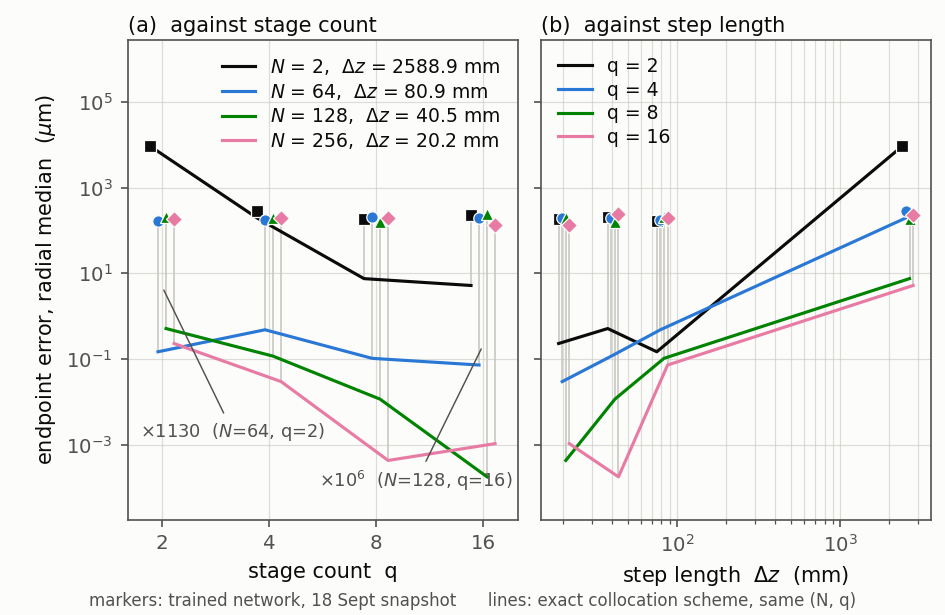
\includegraphics[width=0.9\linewidth]{fig_ceiling.png}
  \caption{The ceiling and the networks. Both panels carry the same sixteen
  $(N, q)$ points twice. The lines are the exact collocation scheme chained $N$
  times and solved without a network, that is the endpoint radial error a
  network of that step count and stage count could reach if its residual were
  driven to zero; the markers are the trained pooled-loss networks at the
  18 September 2026 checkpoint, scored the same way on the same $1452$ test
  tracks, and a thin connector joins each network to its own ceiling. Panel
  (a): against the stage count $q$, one line per step count $N$. Panel (b): the
  same sixteen points against the step length $\Delta z = L/N$, one line per
  $q$. The vertical distance is the point of the figure: for every chain of
  $64$ steps or more the trained network sits two to six orders of magnitude
  above the scheme it is approximating.
  Source: \texttt{scripts/fig03\_ceiling.py}, \texttt{results/fig03\_ceiling.csv}.}
  \label{fig:ceiling}
\end{figure}

\subsection{The sixth-order reference}
\label{sec:scheme-sixthorder}

Everything in this paper is scored against a numerical solution of the equation
of motion, and that solution has to be a number with a bar on it rather than a
convention. The reference is Butcher's seven-stage \emph{explicit} Runge--Kutta
method of order six, in double precision, at a fixed step of $0.1\mm$, marched
plane to plane with the last step of each leg shortened so that the trajectory
lands exactly on the requested plane.

\paragraph{Provenance and identities.} The seven coefficient arrays were copied
from an earlier study's reference machinery and are compared with the original
element by element, with no tolerance: exactly equal, for the nodes, the stage
matrix, the weights, the stated order and the stage count. Each row of $A$ sums
to its node to within $2.2 \times 10^{-16}$, $b$ sums to one with an error of
exactly zero, and $A$ is strictly lower triangular, which is what makes the
method explicit. Four mechanical properties were checked on a leg of $5177.8\mm$,
chosen deliberately not to be a whole number of steps: a forward-then-back
integration on a smooth field closes to $1.8 \times 10^{-12}\mm$; one leg
integrated alone agrees with the same leg inside a mixed batch of five different
legs \emph{exactly}, difference $0.0$, so batching cannot change an answer; a leg
shorter than one step and a zero-length leg both behave, the latter returning the
start state bit for bit; and $q/p$ passes through unchanged.

\paragraph{Order, where order is visible.} The scheme's order was checked on
three problems with exact solutions, chosen so that no single mistake can hide: a
linear one, $dy/dt = -y$, a nonlinear one, $dy/dt = -y^{2}$, and a
non-autonomous one, $dy/dt = y\cos t$, which is the only one that can catch a
wrong node vector. The fitted orders are $6.06$, $6.27$ and $5.75$. Those
problems cannot be pushed through the LHCb integrator, which is hard-wired to
the equation of motion, so the equation was kept and the field replaced by a
smooth analytic stand-in with the same call signature, a Gaussian blob peaking at
$1.05$ T near $z = 4700\mm$. On that field the maximum absolute error against a
fine run is $1.66 \times 10^{-5}$, $2.12 \times 10^{-7}$, $2.93 \times 10^{-9}$
and $4.20 \times 10^{-11}\mm$ at steps of $640$, $320$, $160$ and $80\mm$,
each halving dividing the error by $70$ to $78$ against the ideal $64$. The
\textbf{fitted order is $6.23$}, from the three coarsest points, which are the
ones safely above the arithmetic floor; including the $80\mm$ point as well
gives $6.20$. The ladder has to be that coarse because on a smooth field the
integrator is already at the double-precision floor by an $80\mm$ step.

\paragraph{Order, on the real map, is not visible.} The real map is trilinear on
a $100\mm$ grid and therefore $C^0$: continuous, with a derivative that jumps at
every cell face. A sixth-order scheme integrating across a kink behaves like a
low-order one, and it does.

\begin{table}[tbp]
  \centering
  \caption{The step ladder of the sixth-order reference on the real magnet-up
  map, over $200$ momentum-stratified cross-magnet legs of median span
  $5174\mm$. Left block: how far the endpoint moves when the step is halved.
  Right block: the distance from the finest run of the ladder, at $0.05\mm$.
  Errors are $\max(|\Delta x|, |\Delta y|)$ in micrometres. The last row's two
  blocks coincide because halving $0.1\mm$ \emph{is} the comparison with the
  finest run. Source: \texttt{results/tab\_rk6\_convergence.csv}.}
  \label{tab:rk6ladder}
  \small
  \setlength{\tabcolsep}{6pt}
  \begin{tabular}{rrrrrrr}
    \toprule
    & \multicolumn{3}{c}{$|S(h) - S(h/2)|$ [\um]} & \multicolumn{3}{c}{$|S(h) - S(0.05\mm)|$ [\um]} \\
    \cmidrule(lr){2-4}\cmidrule(lr){5-7}
    $h$ [mm] & median & p95 & max & median & p95 & max \\
    \midrule
    $0.8$ & $9.42\times 10^{-5}$ & $6.41\times 10^{-4}$ & $1.13\times 10^{-3}$ & $1.00\times 10^{-4}$ & $6.79\times 10^{-4}$ & $1.10\times 10^{-3}$ \\
    $0.4$ & $1.18\times 10^{-5}$ & $1.51\times 10^{-4}$ & $2.20\times 10^{-4}$ & $9.78\times 10^{-6}$ & $1.44\times 10^{-4}$ & $2.48\times 10^{-4}$ \\
    $0.2$ & $7.81\times 10^{-6}$ & $5.02\times 10^{-5}$ & $8.17\times 10^{-5}$ & $6.85\times 10^{-6}$ & $3.54\times 10^{-5}$ & $5.91\times 10^{-5}$ \\
    $0.1$ & $2.08\times 10^{-6}$ & $1.64\times 10^{-5}$ & $2.44\times 10^{-5}$ & $2.08\times 10^{-6}$ & $1.64\times 10^{-5}$ & $2.44\times 10^{-5}$ \\
    \bottomrule
  \end{tabular}
\end{table}

The successive ratios of the medians in Table~\ref{tab:rk6ladder} are
$\mathbf{8.0}$, $\mathbf{1.5}$ and $\mathbf{3.8}$, against the $64$ an order-six
method would give. The first of those is the informative one: $8.0 = 2^{3}$ is
exactly what an \textbf{order-three} method gives, and that is what integrating
across kinks turns a sixth-order method into. The size of the penalty can be read
off directly by running the same code on the smooth stand-in field: at
$h = 0.8\mm$ the real map moves the endpoint by $9.4 \times 10^{-5}\um$ per
halving while the smooth field moves it by $9.9 \times 10^{-7}\um$, a factor of
$95$. The trilinear grid costs about two orders of magnitude of accuracy, and no
choice of integrator recovers it; only a smoother field map would.

The remaining two ratios, $1.5$ and $3.8$, are not convergence at all. The smooth
control is the tell: its $0.8 \to 0.2\mm$ difference is $9.9 \times 10^{-7}\um$
but its $0.2 \to 0.05\mm$ difference is \emph{larger}, $4.0 \times
10^{-6}\um$. On a smooth field this scheme is exact to double precision at any of
these steps, so a rising difference can only be rounding accumulating over more
steps, of which there are $103{,}500$ at $0.05\mm$. That sets an arithmetic floor
of a few times $10^{-6}\um$, which the real map's series reaches at
$h = 0.1\mm$. The practical statement is therefore: the endpoint has stopped
moving by $h = 0.2\mm$, and at $h = 0.1\mm$ the series has reached the floor.

\paragraph{Closure.} Integrating each leg forward and back at $0.1\mm$ returns
the start state to a median of $3.66 \times 10^{-6}\um$, a $95$th percentile of
$2.88 \times 10^{-5}\um$ and a worst case of $4.36 \times 10^{-5}\um$ over the
same $200$ legs. \textbf{Closure} is not an accuracy test, because both halves of
the round trip carry the same truncation error and it cancels; it is a floor, and
it agrees with the ladder, both saying a few times $10^{-6}\um$ in the median and
a few times $10^{-5}\um$ in the tail.

\paragraph{The incumbent engine.} Every label in the harvested set and every
experiment before this reference existed was built with double-precision
fourth-order Runge--Kutta at a $5\mm$ step. Against the sixth-order reference at
$0.05\mm$ on these same legs, that engine sits at a median of
$\mathbf{0.0127\um}$, a $95$th percentile of $0.0766\um$ and a worst case of
$0.291\um$; at a $1\mm$ step it sits at $8.2 \times 10^{-4}\um$. Thirteen
nanometres in the median is orders of magnitude below every ceiling and every
network error this paper discusses, so the old engine was never what limited
anything and no earlier result is disturbed. What the fine reference buys is
headroom.

\paragraph{The number to quote.} \textbf{The reference's own floor is
$5 \times 10^{-5}\um$}, that is $0.05$ nm: the worst case over the $200$ legs of
both the step-halving and the closure measurements, rounded up. It is a floor and
not an error bar on any one number. It sits a factor $250$ below the $0.0127\um$
at which the old engine differs from it, and six to seven orders of magnitude
below anything this paper is asked to resolve. Figure~\ref{fig:rk6} draws the
three measurements behind these paragraphs: the order fit on the smooth
stand-in field, the step ladder on the real map, and the levels themselves on
one logarithmic axis.

\paragraph{Cost.} One thread, double precision. The field call is essentially the
whole cost and it amortises over the batch, so the per-track figure falls with
batch size until the map's working set stops fitting in cache: $0.87$ s per track
in a batch of $200$, $0.26$ s at $1000$, $0.134$ s at $5000$ and
$\mathbf{0.12}$ \textbf{s at $20{,}000$}. Measured directly on the $200$-leg
batch it is $1.04$ s per track. Peak resident memory for the whole measurement
was $146$ MB; the cost of this reference is time, not memory.

\begin{figure}[tbp]
  \centering
  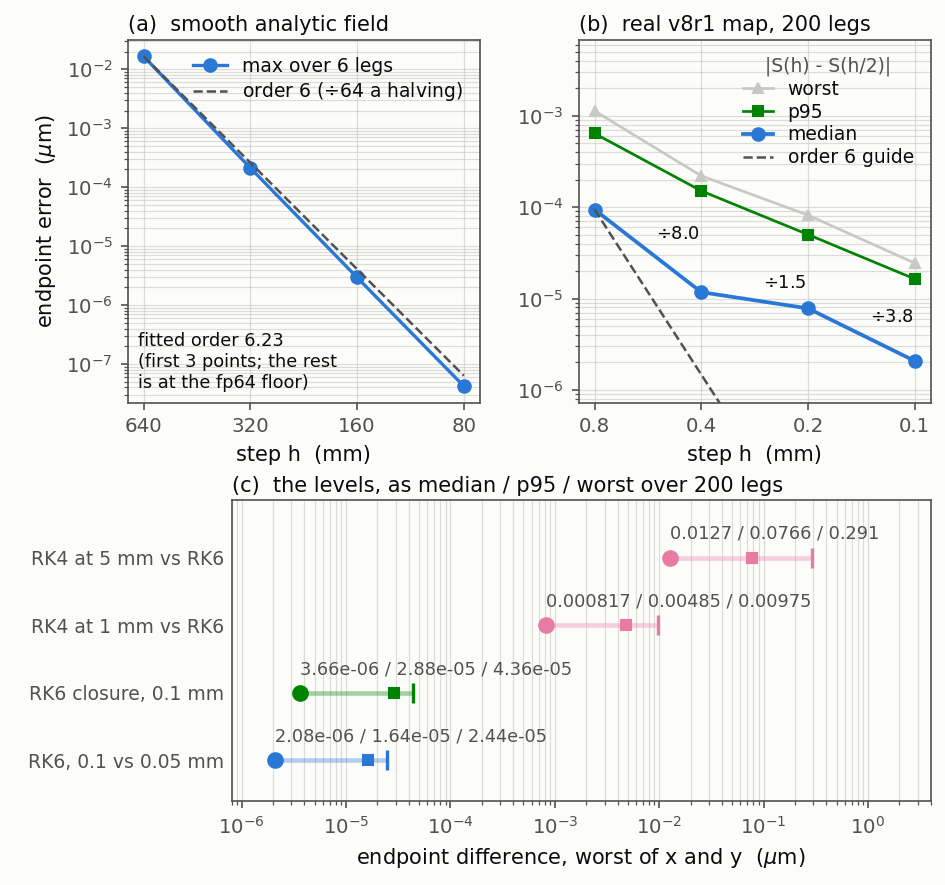
\includegraphics[width=0.9\linewidth]{fig_rk6_reference.png}
  \caption{The sixth-order reference measured on itself. Panel (a): the
  scheme's own order, measured with the trilinear map replaced by a smooth
  analytic stand-in so that the method is not asked to integrate across a kink;
  endpoint error against the same routine at a $0.5\mm$ step, at steps of
  $640$, $320$, $160$ and $80\mm$, with the fitted slope printed and an
  order-six guide drawn through the coarsest point. Panel (b): the step ladder
  on the real magnet-up map, the median, $95$th percentile and worst of
  $|S(h) - S(h/2)|$ over $200$ momentum-stratified cross-magnet legs, with the
  three successive halving ratios $8.0$, $1.5$ and $3.8$ printed beside the
  median line against the $64$ an order-six method would give on a smooth
  field. Panel (c): the levels that matter on one logarithmic axis, what one
  further halving moves the endpoint at the chosen $0.1\mm$ step, what the
  forward-then-back round trip fails to close by at that step, and how far the
  incumbent fourth-order engine at $5\mm$ and at $1\mm$ sits from the fine
  reference, each drawn as median, $95$th percentile and worst.
  Source: \texttt{scripts/fig04\_rk6\_reference.py},
  \texttt{results/fig04\_rk6\_reference.csv}.}
  \label{fig:rk6}
\end{figure}

\subsection{What the field-only reference shares with the truth, and what it cannot}
\label{sec:scheme-fieldonly}

The three preceding subsections establish that the scheme is what I think it
is, that the exact scheme is far below the networks, and that the reference
solves its equation to within $0.05$ nm. None of that answers the question a
supervisor asks next: the reference is a solution of an equation, but is the
equation what the simulated particle actually did? This subsection measures the
answer on all $14{,}482$ crossings, takes the gap apart into physical pieces with
two tests rather than assertions, and says which pieces are removable.

I say at the outset what does and does not follow. \textbf{The networks of this
paper are measured against the sixth-order reference, and the gap measured here
does not enter any network number.} The network and the reference solve the same
equation with the same $q/p$; they share every omission. What this subsection
sets is the ceiling of the programme: the level at which a field-only
extrapolator, however perfect, stops agreeing with the simulation. The comparison
of the networks themselves against the simulated truth belongs in
Section~\ref{sec:results-truth}.

\paragraph{The three objects.} Three different states exist on the first
fibre-tracker plane for one and the same particle.
\begin{enumerate}\setlength{\itemsep}{2pt}
  \item \textbf{The simulated truth.} Geant4 records a Monte Carlo hit wherever
  a particle crosses a sensitive volume, and I build a state from the midpoint of
  its entry and exit points and from the entry-to-exit displacement over its own
  $\Delta z$. The inverse momentum attached to that state comes not from the hit
  but from the particle record, that is the momentum the particle had \emph{when
  it was produced}; that detail is the origin of the largest single piece of what
  follows. The state contains everything the simulation did to the particle,
  scattering and ionisation loss included, and no detector effect at all: there
  is no digitisation and no reconstruction anywhere in this paper.
  \item \textbf{The field-only reference.} The particle's real state on its last
  Upstream Tracker plane, carried to $z_0$, integrated across the magnet and on
  to that particle's own fibre-tracker plane with the sixth-order integrator at
  $0.1\mm$. The equation holds $d(q/p)/dz = 0$: the momentum is constant along
  the whole crossing, the field is the only thing in the equation, and there is
  no material of any kind.
  \item \textbf{The network endpoint.} One network applied $N$ times from the
  same real state, trained on the residual of that same equation. Whatever the
  equation omits, the network omits by construction.
\end{enumerate}
Since the tracker is not one flat plane, each particle's own $z_{\mathrm{post}}$
differs from $z_1$ by at most $7.45\mm$. Both the reference state and the network
state at $z_1$ are therefore carried from $z_1$ to that particle's own plane with
the same integrator before any comparison is made.

\paragraph{Why this was not visible earlier.} The labels were gated against the
simulation when they were built, and the gate looked reassuring: on $100{,}660$
short plane-to-plane legs the label disagreed with the particle's own next hit by
a median of $11.9\um$, falling to $3.8\um$ above $5$ GeV and rising to $38.8\um$
below $2$ GeV. Those legs are short and the magnet crossing is not. The
difference is the lever arm: a slope error of $10^{-4}$ displaces a track by
$10\um$ over a $10$ cm gap between two tracker planes and by $518\um$ over the
$5177.8\mm$ of the crossing, so the same physics is fifty times larger here.

\paragraph{Test one: what happens under a charge flip.} Write
$\Delta = S_{\mathrm{true}} - S_{\mathrm{ref}}$ at the particle's own plane. The
charge enters the equation of motion only through $q/p$, and it enters the two
slope derivatives linearly. If the momentum handed to the integrator is too large
by a relative amount $\epsilon = \Delta p / p$, every slope derivative is scaled
by $(1 + \epsilon)$ and, to first order, so is the whole bend. Define the bend
\begin{equation}
  b \;=\; x_{\mathrm{ref}}(z_{\mathrm{post}}) - \bigl[x_0 + t_{x,0}(z_{\mathrm{post}} - z_0)\bigr],
\end{equation}
where $x_0$ and $t_{x,0}$ are the start position and slope: the horizontal
distance between where the reference ends up and where a straight line through
the start state would have put it, that is the magnet's whole effect on that
track. Its median magnitude over this set is $453\mm$, and $14{,}476$ of the
$14{,}482$ tracks have $|b| > 20\mm$, which is the cut applied whenever I divide
by it. Then
\begin{equation}
  \Delta x \;\approx\; \epsilon\, b \quad \text{flips sign with the charge,}
  \qquad\text{while}\qquad
  \frac{\Delta x}{b} \;\approx\; \epsilon \quad \text{does not.}
\end{equation}
Multiple scattering has no such structure: a scattered particle is as likely to
go left as right whatever its charge, so it contributes nothing to the
\emph{median} of $\Delta x$ for either charge and shows up only in the
charge-blind \emph{width}. Splitting the set by charge therefore separates a
bending systematic from random scattering with no modelling assumption. A worked
micro-example: a $5$ GeV track that bends by $500\mm$ and whose reference misses
by $2500\um$ in $x$ has $\Delta x / b = 5 \times 10^{-3}$, which reads as a
momentum defect of $5 \times 10^{-3} \times 5\ \mathrm{GeV} = 25$ MeV.

Reading $\Delta x / b$ as a momentum also distinguishes two candidate causes. If
the implied defect is a \emph{fixed number of MeV} independent of momentum, that
is what ionisation energy loss looks like: a particle of any momentum loses
roughly the same absolute amount crossing the same material. If instead the
\emph{ratio} were constant across momentum, that would point at the field rather
than the momentum, because a field map scaled wrongly by a fixed fraction
produces a fixed relative over-bend at every momentum.

\paragraph{Test two: the width against Highland.} For the random part I compare
the measured width with what multiple Coulomb scattering should give. The
standard parameterisation is Highland's \citep{lynch1991},
\begin{equation}
  \theta_0 \;=\; \frac{13.6\ \mathrm{MeV}}{\beta c\, p}\, z_{\mathrm{ch}}
  \sqrt{\frac{x}{X_0}}\left[1 + 0.038 \ln\!\left(\frac{x}{X_0}\right)\right],
  \label{eq:highland}
\end{equation}
where $\theta_0$ is the root-mean-square scattering angle projected onto one
plane, $p$ is the momentum, $\beta c$ the velocity, which is $c$ to an excellent
approximation for every track here since the slowest is $1.5$ GeV,
$z_{\mathrm{ch}} = 1$ is the charge in units of the elementary charge, and
$x/X_0$ is the thickness traversed in \textbf{radiation lengths}. A radiation
length $X_0$ is the material thickness in which an electron loses all but $1/e$
of its energy to bremsstrahlung, and it is the natural unit in which scattering
is quoted; for air it is about $304$ m. A particle scattering continuously over a
length $L$ ends up displaced sideways by
\begin{equation}
  \sigma_{\mathrm{displacement}} \;\approx\; \frac{\theta_0 L}{\sqrt{3}},
\end{equation}
the $\sqrt{3}$ arising because deflections earned near the end of the path have
almost no lever arm left to act over. The only material between the two planes
that can be accounted for from first principles is the air: $L = 5177.8\mm$
against $X_0 = 304$ m gives $x/X_0 = 0.01703$, that is $1.70$ per cent of a
radiation length. I compute the prediction at each band's median momentum,
compare it with the measured width, and invert Eq.~\eqref{eq:highland}
numerically for the thickness the measured width implies.

Because the two charges have systematically different centres, pooling them
carelessly would let the systematic inflate the width. I therefore move each
charge onto its own median first, then pool, then take the $68$th percentile of
the absolute deviation from that centre. That is the statistic called ``$68$ per
cent half-width'' below.

\paragraph{The decomposition, band by band and charge by charge.}
Table~\ref{tab:decomp} is the main measurement, on all $14{,}482$ crossings,
re-binned into this paper's five bands.

\begin{table}[tbp]
  \centering
  \caption{The simulated truth minus the field-only reference at each particle's
  own first fibre-tracker plane, on all $14{,}482$ crossings, in the paper's
  bands. Columns: the band population split by charge; the signed median of
  $\Delta x$ for each charge, which flips sign; the median of $\Delta x / b$ for
  each charge, which does not; the momentum defect that ratio implies, computed
  as the pooled median ratio times the band's median momentum; and the
  charge-corrected $68$ per cent half-width of $\Delta x$. Positions in
  micrometres. The row marked ``window'' is the $10$--$50$ GeV loss window, which overlaps two bands and is not part of the partition. \textbf{This table is
  the original study's Table~4.2 re-binned into the paper's bands}; its content
  is the same measurement on the same crossings.
  Source: \texttt{results/tab\_decomposition\_bands.csv} and
  \texttt{results/paper\_numbers.json} (\texttt{reference\_vs\_truth.rebinned\_decomposition}).}
  \label{tab:decomp}
  \footnotesize
  \setlength{\tabcolsep}{4pt}
  \begin{tabular}{lrrrrr}
    \toprule
    band & $n$ & median $\Delta x$ & median $\Delta x / b$ & implied $\Delta p$ & $68\%$ half-width \\
    $[$GeV$]$ & ($q^{+}/q^{-}$) & [\um], $q^{+}/q^{-}$ & [$10^{-3}$], $q^{+}/q^{-}$ & [MeV] & of $\Delta x$ [\um] \\
    \midrule
    $<3$       & $1684$ ($880/804$)     & $-8641 / +8130$ & $+6.90 / +6.53$   & $+17.6$ & $6119$ \\
    $3$--$8$   & $6606$ ($3442/3164$)   & $-2277 / +2151$ & $+3.62 / +3.50$   & $+17.3$ & $2676$ \\
    $8$--$20$  & $4265$ ($2171/2094$)   & $-257 / +245$   & $+1.08 / +0.974$  & $+12.2$ & $815$ \\
    $20$--$50$ & $1650$ ($801/849$)     & $+14 / -7$      & $-0.149 / -0.0712$& $-3.1$  & $351$ \\
    $>50$      & $277$ ($145/132$)      & $+51 / -58$     & $-1.22 / -1.42$   & $-86.8$ & $160$ \\
    \midrule
    $10$--$50$ (window) & $4713$ ($2366/2347$) & $-71 / +74$ & $+0.443 / +0.470$ & $+7.5$ & $582$ \\
    \midrule
    all        & $14{,}482$ ($7439/7043$) & $-1032 / +873$ & $+2.65 / +2.37$ & $+17.0$ & $2262$ \\
    \bottomrule
  \end{tabular}
\end{table}

Read with test one in mind, the table says three things at once.

First, \textbf{the signed median flips sign with the charge and the ratio to the
bend does not.} In the $3$--$8$ GeV band a positive particle is found $2277\um$
to one side of the reference and a negative particle $2151\um$ to the other,
while both give $\Delta x / b \approx +3.6 \times 10^{-3}$. That is the signature
of a momentum error and of nothing else. Scattering cannot produce it, because
scattering has no preferred side. Note also how small the pooled signed median
is once the two charges are added together, $-205\um$ in that band against
$\pm 2200\um$ per charge: a pooled analysis would have seen almost nothing.

Second, \textbf{below $20$ GeV the implied defect is a roughly constant number
of MeV and not a constant fraction.} It is $+17.6$, $+17.3$ and $+12.2$ MeV in
the three lowest bands and $+7.5$ MeV in the loss window, while the relative
ratio $\Delta x / b$ falls by a factor of six over the same range. A fixed absolute momentum loss is what ionisation energy loss looks like
and is not what a field-scale error looks like. The simulated particle really is
slower than the number handed to the integrator, by of order $17$ MeV, because
the start state carries the particle's \emph{production} momentum: the state
harvesting joins the momentum from the particle table, and the truth dump never
wrote the hit's own local momentum, which Geant4 records and which my dump
simply did not ask for. What the $17$ MeV contains is the energy the particle
lost in the vertex detector and the Upstream Tracker before reaching the start
plane, plus the energy it loses in the crossing itself, which the integrator also
does not model. The two cannot be separated without re-dumping the truth, and
that is the first of the two loose ends in item 6 of
Section~\ref{sec:outlook}.

Third, \textbf{above $20$ GeV the sign reverses and the ratio grows.} The
implied defect becomes $-3.1$ MeV in the $20$--$50$ GeV band and $-86.8$ MeV
above $50$ GeV, a relative under-bend of $0.01$ and $0.13$ per cent. A defect
that grows with momentum is not energy loss. I state this as unexplained and
name the candidates without choosing: a difference between the map I integrate
in and the map and current the simulation was run with under its conditions tag,
a scale difference of a tenth of a per cent being exactly the right size; or the
accuracy of Geant4's own field stepper. The two bands hold $1650$ and $277$
crossings across all three splits, and only $170$ and $30$ of those are in the
test split, so the high-momentum statement in particular carries little weight.
In the original study's finer binning the same quantity reads $-8.1$ MeV at
$25$--$50$ GeV, $-77.5$ MeV at $50$--$100$ GeV and $-240.4$ MeV at
$100$--$200$ GeV, over $1016$, $240$ and $37$ crossings, which shows the growth
more clearly than the paper's coarser bands can.

\paragraph{The random part.} Table~\ref{tab:highland} puts the last column of
Table~\ref{tab:decomp} against Eq.~\eqref{eq:highland} for air alone.

\begin{table}[tbp]
  \centering
  \caption{The charge-corrected $68$ per cent half-width of $\Delta x$ against
  the Highland prediction for the air between the two planes, on all $14{,}482$
  crossings, in the paper's bands. The air thickness is
  $x/X_0 = 5177.8\mm / 304\ \mathrm{m} = 0.01703$ everywhere. The last column
  inverts Eq.~\eqref{eq:highland} for the thickness the measured width implies,
  which is a measurement of the simulation's material budget and not a
  confirmation of anything, since I have not looked that budget up
  independently. Source: \texttt{results/tab\_highland\_air.csv}.}
  \label{tab:highland}
  \footnotesize
  \setlength{\tabcolsep}{4pt}
  \begin{tabular}{lrrrrrrr}
    \toprule
    band [GeV] & $n$ & median $p$ & $\theta_0$, air & air, Eq.~\eqref{eq:highland}
      & measured & ratio & implied \\
    & & [GeV] & [$\mu$rad] & [\um] & [\um] & & $x/X_0$ \\
    \midrule
    $<3$       & $1684$ & $2.63$   & $571$  & $1706$ & $6119$ & $3.59$ & $0.179$ \\
    $3$--$8$   & $6606$ & $4.84$   & $310$  & $926$  & $2676$ & $2.89$ & $0.120$ \\
    $8$--$20$  & $4265$ & $11.95$  & $125.6$& $375$  & $815$  & $2.17$ & $0.071$ \\
    $20$--$50$ & $1650$ & $27.28$  & $55.0$ & $164$  & $351$  & $2.14$ & $0.069$ \\
    $>50$      & $277$  & $65.49$  & $22.9$ & $68$   & $160$  & $2.34$ & $0.081$ \\
    \midrule
    $10$--$50$ (loss window) & $4713$ & $16.40$ & $91.5$ & $273$ & $582$ & $2.13$ & $0.068$ \\
    \bottomrule
  \end{tabular}
\end{table}

Above $8$ GeV the measured width is a stable $2.1$ to $2.3$ times the air-only
prediction, and the thickness it implies is a stable $6.8$ to $8.1$ per cent of a
radiation length against the $1.70$ per cent that air alone provides. The
simulation therefore puts about four times more scattering material between the
two planes than the air does, which is entirely plausible: the magnet region is
not empty, and the last Upstream Tracker and first fibre-tracker stations have
structure of their own. Below $8$ GeV the ratio climbs to $2.9$ and $3.6$.
Highland's parameterisation describes the Gaussian core and degrades in exactly
that regime, where the non-Gaussian single-scattering tail is large and where a
$68$ per cent half-width begins to sample it, so I do not read the two softest
rows as evidence of more material.

\paragraph{The particle-type cross-check.} If the systematic really is energy
loss, then at the same momentum the over-bend should order itself by particle
mass, because ionisation loss depends on velocity. Table~\ref{tab:pid} is that
test.

\begin{table}[tbp]
  \centering
  \caption{The over-bend by particle type, measured at $5$--$25$ GeV with the
  bend cut applied. This table is quoted in the original study's own selection
  and binning, because no re-binned version exists. The ordering pion, kaon,
  proton is the one an energy-loss explanation predicts; the muons carry no
  statistical weight. Source:
  \texttt{single\_network\_chain\_discrete\_approach/}\allowbreak\texttt{reference\_vs\_truth/results/decomposition\_by\_pid.csv},
  via \texttt{results/paper\_numbers.json}
  (\texttt{reference\_vs\_truth.verbatim.decomposition\_by\_pid}).}
  \label{tab:pid}
  \small
  \setlength{\tabcolsep}{6pt}
  \begin{tabular}{lrrrrr}
    \toprule
    particle & $n$ & median $p$ [GeV] & median $\Delta x / b$
      & median $|\Delta x|$ [\um] & implied $\Delta p$ [MeV] \\
    \midrule
    pion   & $6139$ & $9.25$  & $+1.65\times 10^{-3}$ & $811$ & $+15.3$ \\
    kaon   & $909$  & $10.44$ & $+1.48\times 10^{-3}$ & $698$ & $+15.4$ \\
    proton & $893$  & $9.82$  & $+1.23\times 10^{-3}$ & $395$ & $+12.1$ \\
    muon   & $42$   & $7.40$  & $+1.11\times 10^{-3}$ & $811$ & $+8.2$  \\
    \bottomrule
  \end{tabular}
\end{table}

The ordering is the predicted one and the effect is modest, about $25$ per cent
in the ratio between pion and proton. I record it as consistent with an
energy-loss explanation and do not push it further; only a rebuilt truth dump
carrying the local momentum can make this test sharp.

\paragraph{The slopes say the same thing.} Everything above is about position.
The slope residuals behave identically, which is what a single physical cause
requires. Over all $14{,}482$ crossings with both charges pooled, the median
absolute slope residual is $3.68 \times 10^{-4}$ in $t_x$ and $2.20 \times
10^{-4}$ in $t_y$; below $3$ GeV it is $3.31 \times 10^{-3}$ and $7.37 \times
10^{-4}$, and above $50$ GeV it is $3.11 \times 10^{-5}$ and $1.92 \times
10^{-5}$. Two features are worth naming. At low momentum the horizontal residual
is about four times the vertical one in position and four to five times in slope,
because the magnet bends in $x$ and the momentum systematic therefore appears
there and not in $y$. Above $20$ GeV, where the systematic has largely gone, the
two components converge, which is what a purely random cause requires: at
$20$--$50$ GeV the median absolute residuals are $204\um$ in $x$ against $219\um$
in $y$ and $6.19 \times 10^{-5}$ in $t_x$ against $5.69 \times 10^{-5}$ in $t_y$.

\paragraph{What the reference does agree with.} Table~\ref{tab:rk6self} collects
the self-consistency numbers in one place, so that the size of the gap to the
simulation can be read against the size of everything the reference \emph{can}
be checked against.

\begin{table}[tbp]
  \centering
  \caption{The reference against itself and against the schemes, beside the two
  comparators that bracket the problem. All entries are endpoint errors in
  micrometres; the exact-scheme and comparator rows are radial medians on the
  $1452$ test tracks and the rest are as noted in the $n$ column. The three
  \emph{label against the particle's next hit} rows, including the $>5$ GeV and
  $<2$ GeV rows, are quoted in the original study's own selection and binning,
  because no re-binned version exists. Source:
  \texttt{single\_network\_chain\_discrete\_approach/}\allowbreak\texttt{reference\_vs\_truth/results/rk6\_self\_consistency.csv},
  via \texttt{results/paper\_numbers.json}
  (\texttt{reference\_vs\_truth.verbatim.rk6\_self\_consistency}).}
  \label{tab:rk6self}
  \small
  \setlength{\tabcolsep}{6pt}
  \begin{tabular}{lrr}
    \toprule
    quantity & value [\um] & $n$ \\
    \midrule
    closure of the integrator, forward then back, median & $2.3\times 10^{-6}$ & $2000$ \\
    closure of the integrator, worst case                & $22.4$      & $2000$ \\
    step convergence, $5\mm$ against $1\mm$, median      & $2.8\times 10^{-5}$ & $200$ \\
    step convergence, worst case                         & $2.8$       & $200$ \\
    label against the particle's next hit, short legs, median & $11.9$ & $100{,}660$ \\
    the same, above $5$ GeV                              & $3.8$       & $100{,}660$ \\
    the same, below $2$ GeV                              & $38.8$      & $100{,}660$ \\
    exact scheme, $N = 64$, $q = 2$, $\Delta z = 80.9\mm$  & $0.147$     & $1452$ \\
    exact scheme, $N = 128$, $q = 8$, $\Delta z = 40.5\mm$ & $0.0115$    & $1452$ \\
    exact scheme, $N = 256$, $q = 16$, $\Delta z = 20.2\mm$& $1.05\times 10^{-3}$& $1452$ \\
    \midrule
    straight line, no magnet at all                      & $450{,}542$ & $1452$ \\
    the simulated truth against the reference            & $1896$      & $1452$ \\
    \bottomrule
  \end{tabular}
\end{table}

The reading is stark. Sub-micrometre closure, picometre step convergence and
sub-micrometre agreement with the exact collocation scheme leave no room for
integration error anywhere near the millimetre scale. The reference solves its
equation essentially exactly. The equation is what is incomplete, and the
$1736\um$ median gap to the simulation, $1896\um$ in the radial metric on the
test split, is that incompleteness and nothing else.
Figure~\ref{fig:materialgap} separates that gap into the charge-odd systematic
and the charge-blind width, band by band.

\begin{figure}[tbp]
  \centering
  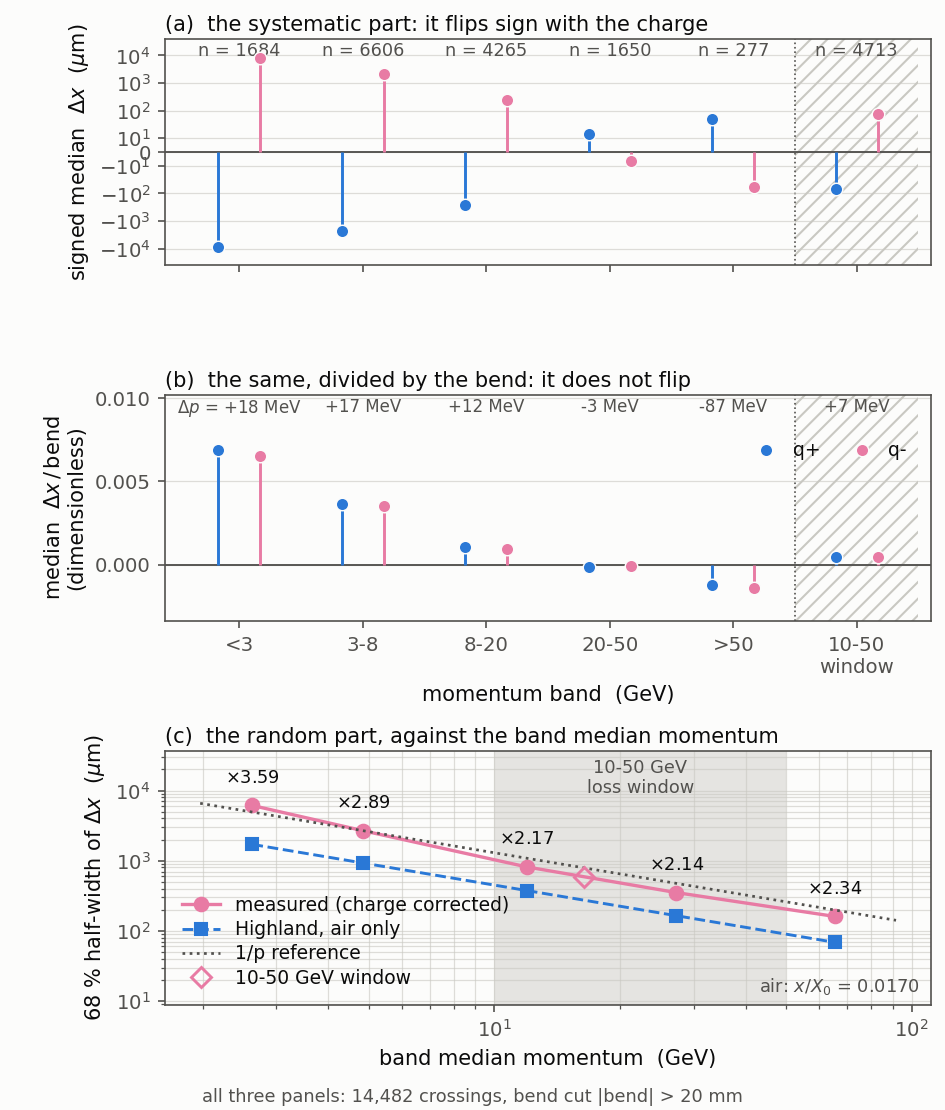
\includegraphics[width=0.9\linewidth]{fig_material_gap.png}
  \caption{What separates the field-only reference from the real particle, on
  all $14{,}482$ crossings. Panel (a): the systematic part, the signed median of
  $\Delta x$ per momentum band drawn separately for positive and negative
  tracks, on a symmetric logarithmic axis so that the four orders of magnitude
  between the softest and the stiffest band are all visible; below $20$ GeV the
  two charges sit on opposite sides of zero, which is what a charge-odd effect
  looks like. Panel (b): the same quantity divided by each track's own bend.
  The ratio is dimensionless and is plotted at its own scale, multiplied by
  nothing. It does not flip sign with the charge, which is the signature of a
  momentum defect, and the defect it implies is printed above each band to the
  nearest MeV: $+18$, $+17$ and $+12$ MeV below $20$ GeV, then $-3$ and $-87$
  MeV in the two stiffest bands and $+7$ MeV for the loss window. Panel (c): the random part, the charge-corrected
  $68$ per cent half-width of $\Delta x$ against the band's median momentum on
  logarithmic axes, beside Highland's prediction for the air between the two
  planes and a pure $1/p$ line anchored on the $3$--$8$ GeV measurement; the
  measured width is a factor $2.14$ to $3.59$ wider than air alone over the five
  bands, and that ratio is printed at each of those five points.
  Source: \texttt{scripts/fig06\_material\_gap.py},
  \texttt{results/fig06\_material\_gap.csv}.}
  \label{fig:materialgap}
\end{figure}

\paragraph{What this means for the programme.} The gap has three parts and a
remainder, and they have different status.
\begin{enumerate}\setlength{\itemsep}{2pt}
  \item \textbf{The start momentum is the production momentum}, not the momentum
  the particle had at the Upstream Tracker. This is a defect in my own data
  pipeline and not physics, and it is fixable cheaply: it shows as a
  charge-antisymmetric over-bend worth $+17.6$, $+17.3$ and $+12.2$ MeV in the
  three bands below $20$ GeV.
  \item \textbf{Energy loss along the crossing itself.} The equation holds $q/p$
  constant; a real particle loses energy continuously. This is deterministic and
  therefore addable to the equation, which is what LHCb's production extrapolator
  does in a separate material layer. Part of the $17$ MeV belongs here rather
  than to the start plane, and only a rebuilt dataset will say how it splits.
  \item \textbf{Multiple Coulomb scattering.} Random, charge-blind, falling as
  $1/p$, measured here at $582\um$ of half-width in the $10$--$50$ GeV loss
  window and about $2.1$ times the air-only estimate. This is stochastic and
  therefore irreducible for any deterministic reference. A deterministic
  extrapolator can predict its variance and propagate it as a covariance, which
  is exactly what a Kalman filter does with it, but it can never predict the
  individual deflection. No extra Runge--Kutta order, no extra collocation stage
  and no extra network capacity can touch it.
  \item Separately from these three, the \textbf{momentum-growing residual above
  $20$ GeV}, which I have not explained.
\end{enumerate}

Nothing in the network studies moves because of any of this: the networks and the
reference share the same equation and the same $q/p$, so every
network-against-reference number in Section~\ref{sec:results} is unaffected.
What this subsection fixes is the level at which the programme stops being about
integration and starts being about physics the equation was never given: about
$1.7\mm$ in the median over this sample, $532\um$ in the loss window, and
$153\um$ above $50$ GeV.

% ===========================================================================
\section{Results}
\label{sec:results}

This section reports the experiment. It is long because there are two losses,
three step lengths and six trained networks, and because the interesting part
of the answer is not the headline number but the way the improvement is
distributed. I take the pieces in the order in which they were measured.
Section~\ref{sec:results-grid} lays out the sixteen networks trained under the
pooled loss of Eq.~\eqref{eq:pooled} over a grid of step counts and stage
counts, which is what fixed the three working points the rest of the paper
uses. Section~\ref{sec:results-weight} is the pre-flight: where each of the two
objectives actually spends itself, measured on a trained network before any
reweighted network existed, together with the scan that chose the clamp.
Section~\ref{sec:results-plateau} says which of the six runs had finished
training and which had not, because that determines what the comparison is
allowed to claim. Section~\ref{sec:results-headline} is the comparison itself,
three networks under two losses, and the test of the criterion that was fixed
in advance. Section~\ref{sec:results-components} takes the endpoint error apart
by state component and by momentum band, Section~\ref{sec:results-5gev} looks
closely at the region around $5$ GeV, and
Section~\ref{sec:results-anatomy} decomposes what is left into per-step errors
and their accumulation. Section~\ref{sec:results-shortersteps} asks what
shorter steps bought, Section~\ref{sec:results-truth} sets every number against
the simulated truth rather than against the reference, and
Section~\ref{sec:results-cost} reports what all of it cost to train and what a
trained network costs to run.

Every number in this section is measured on the $1{,}452$ test tracks unless it
says otherwise, and every error is against the sixth-order reference of
Section~\ref{sec:theory-references} carried to the first SciFi plane unless it
says otherwise. The statistics are those defined in
Section~\ref{sec:theory-metrics} and are not redefined here. The three networks
that carry the comparison are named by their step count, their stage count and
their step length --- $N = 64$, $q = 2$, $\Delta z = 80.9\mm$;
$N = 128$, $q = 8$, $\Delta z = 40.5\mm$; and $N = 256$, $q = 16$,
$\Delta z = 20.2\mm$ --- and after this paragraph the step count and the stage
count alone identify them.

% ---------------------------------------------------------------------------
\subsection{The pooled loss over the grid of step counts and stage counts}
\label{sec:results-grid}

The first question is whether chaining one network to itself works at all, and
at what step length and stage count it works best under the objective the
construction comes with; Table~\ref{tab:grid} is the sixteen-run answer.

\begin{table}[tbp]
  \centering
  \caption{The sixteen networks trained under the pooled loss of
  Eq.~\eqref{eq:pooled}, one per combination of step count $N$ and stage count
  $q$, scored on the $1{,}452$ test tracks. \emph{Endpoint} is the chain of $N$
  applications from the track's real Upstream Tracker state, radial metric at
  $z_1$. \emph{Ceiling} is the same $q$-stage scheme at the same step length,
  chained the same $N$ times and solved directly by a root-finder with no
  network anywhere, from Table~\ref{tab:ceiling}. \emph{Single step} is one
  application of the same network from a reference state on an interior plane,
  median over all planes and tracks. \textbf{This table, and only this table,
  uses the stopped snapshot of 18 September 2026}; none of these runs had
  plateaued when it was taken (Section~\ref{sec:results-plateau}), so the
  ordering within the grid is a snapshot and not a ranking. The three
  combinations carried forward are marked $\star$. Source:
  \texttt{results/tab\_pooled\_grid.csv} and
  \texttt{results/tab\_exact\_ceiling.csv}.}
  \label{tab:grid}
  \footnotesize
  \setlength{\tabcolsep}{5pt}
  \begin{tabular}{rrrrrrrr}
    \toprule
    $N$ & $q$ & $\Delta z$ [\!\mm] & endpoint med. [\!\um] &
    endpoint p95 [\!\um] & ceiling [\!\um] & single step [\!\um] &
    restarts \\
    \midrule
    $2$   & $2$  & $2588.9$ & $9{,}250$ & $39{,}347$ & $9{,}270.9$   & $1{,}430.8$ & $109$ \\
    $2$   & $4$  & $2588.9$ & $283.8$   & $2{,}011$  & $195.40$      & $92.46$     & $159$ \\
    $2$   & $8$  & $2588.9$ & $188.1$   & $1{,}428$  & $7.472$       & $62.53$     & $130$ \\
    $2$   & $16$ & $2588.9$ & $223.6$   & $1{,}683$  & $5.167$       & $72.81$     & $106$ \\
    \midrule
    $64$  & $2$  & $80.90$  & $166.3$   & $1{,}154$  & $0.1465$      & $0.4151$    & $760$ \ $\star$ \\
    $64$  & $4$  & $80.90$  & $172.4$   & $1{,}051$  & $0.4783$      & $0.5568$    & $714$ \\
    $64$  & $8$  & $80.90$  & $204.2$   & $1{,}249$  & $0.1030$      & $0.6477$    & $657$ \\
    $64$  & $16$ & $80.90$  & $194.2$   & $1{,}207$  & $0.0719$      & $0.8103$    & $546$ \\
    \midrule
    $128$ & $2$  & $40.45$  & $207.0$   & $1{,}206$  & $0.5107$      & $0.1509$    & $760$ \\
    $128$ & $4$  & $40.45$  & $195.6$   & $1{,}246$  & $0.1159$      & $0.2567$    & $713$ \\
    $128$ & $8$  & $40.45$  & $158.6$   & $1{,}090$  & $0.0115$      & $0.3086$    & $599$ \ $\star$ \\
    $128$ & $16$ & $40.45$  & $246.2$   & $1{,}410$  & $0.000176$    & $0.3739$    & $383$ \\
    \midrule
    $256$ & $2$  & $20.23$  & $185.3$   & $1{,}319$  & $0.2284$      & $0.0906$    & $758$ \\
    $256$ & $4$  & $20.23$  & $195.6$   & $1{,}275$  & $0.0295$      & $0.0854$    & $709$ \\
    $256$ & $8$  & $20.23$  & $193.6$   & $1{,}204$  & $0.000426$    & $0.1276$    & $615$ \\
    $256$ & $16$ & $20.23$  & $136.8$   & $1{,}082$  & $0.00105$     & $0.0944$    & $550$ \ $\star$ \\
    \bottomrule
  \end{tabular}
\end{table}

Read it this way. The four rows at $N = 2$ are the control, and they reproduce
the first paper's central demonstration on a completely different geometry. At
$N = 2$, $q = 2$ the chained network lands at $9{,}250\um$ against a ceiling of
$9{,}271\um$: the two agree to $0.2$ per cent. The network is not failing
there. It is solving the equations it was given, and a two-stage
Gauss--Legendre scheme taking two steps of $2589\mm$ through the magnet is
itself $9\mm$ wrong. At $q = 4$ the ceiling drops to $195\um$ and the network
sits at $284\um$, a factor $1.45$ above it. From $q = 8$ onwards the ceiling
falls through $7.5\um$ to $5.2\um$ while the network stops at $188$ and
$224\um$: the discretisation has stopped being the limitation and the optimiser
has become it. That is the same crossing the first paper reported on its single
frozen leg, and it happens here at the same stage count.

The twelve rows at $N \geq 64$ are the experiment proper, and the first thing
to say about them is that the ceiling is irrelevant. The exact scheme chained
$64$, $128$ or $256$ times lands between $0.000176\um$ and $0.51\um$ of the
reference, so every one of those twelve networks sits between two and six
orders of magnitude above the answer its own objective is pointing at. Nothing
in this part of the grid is limited by the numerical scheme; everything is
limited by how well the network solves it. That is the single most useful fact
in the table, because it means the rest of the paper is about optimisation and
about the objective, not about discretisation error.

The second thing to say is that the twelve endpoint medians do not order
themselves. They run from $136.8\um$ at $N = 256$, $q = 16$ to $246.2\um$ at
$N = 128$, $q = 16$, a total spread of a factor $1.80$, with no monotone trend
in either $N$ or $q$ and with the best and the worst run sharing a stage count.
The single-step column behaves quite differently: it falls smoothly with the
step, from $0.42$--$0.81\um$ at $N = 64$ through $0.15$--$0.37\um$ at $N = 128$
to $0.085$--$0.13\um$ at $N = 256$. One application of the network gets steadily
better as the step gets shorter, and the chain of $N$ of them does not. That
gap is the subject of Sections~\ref{sec:results-anatomy}
and~\ref{sec:results-shortersteps}, and it is the reason the paper does not
simply recommend the shortest step available.

It is worth one sentence on how small the single-step numbers are in context.
Ignoring the magnet and continuing along the incoming slopes over one step of
$80.90\mm$ costs $95.2\um$; over $40.45\mm$ it costs $23.8\um$; over
$20.23\mm$ it costs $5.96\um$. The single-step errors above are therefore
between $0.44$ and $0.85$ per cent of the straight line at $N = 64$ and
between $1.4$ and $2.1$ per cent at $N = 256$. A single application of any of
these networks is a good step. It is the chaining that costs.

Three combinations were carried forward into the comparison, marked $\star$ in
the table: $N = 64$ with $q = 2$, $N = 128$ with $q = 8$ and $N = 256$ with
$q = 16$. The choice pairs each halving of the step with a doubling of the
stage count, so that the three points differ in step length while keeping the
per-step arithmetic growing in a controlled way, and the middle point is the
grid's best run at that step length. The three were fixed before any
reweighted network was trained. Because the runs in Table~\ref{tab:grid} were
all stopped short, every one of the three was afterwards extended to its own
plateau before being used as a counterpart, and it is those extended runs, not
these, that appear in every later table.

% ---------------------------------------------------------------------------
\subsection{Where each loss puts its weight}
\label{sec:results-weight}

Before any reweighted network was trained, both objectives were evaluated on
the same trained network and the same states, so that the difference between
them could be described rather than assumed; this section reports that
measurement, the ablations that attribute it to the three factors of
Eq.~\eqref{eq:lossF}, and the scan that chose the clamp.

The measurement is the one already quoted in Section~\ref{sec:theory-pooled}
and is set out in full in Table~\ref{tab:preflight}. Eight thousand
$(\text{track}, \text{plane})$ states were drawn evenly over the $64$ start
planes of the extended $N = 64$, $q = 2$ network, the residuals of
Eq.~\eqref{eq:resid} were formed once, and each state's share of the total
loss was accumulated under five weighting modes.\footnote{An earlier record of
this pre-flight exists and was taken on the stopped checkpoint of 18 September
2026 rather than on the extended network. The quantities that record stored are
carried in the companion file of Figure~\ref{fig:lossshares} as a separate
column: it gives, for the pooled loss, a rank correlation of $0.690$ overall
and $0.559$ in the window against $0.684$ and $0.532$ here, a top-one-per-cent
share of $97.9$ against $98.3$ per cent, and first- and last-quarter shares of
$0.556$ and $6.15$ against $0.650$ and $6.22$ per cent; for the cost-weighted
loss it gives $0.561$ and $0.889$, $83.8$ per cent, and $21.2$ and $1.75$ per
cent. Re-running the pre-flight on that checkpoint reproduces the stored record
exactly, to zero deviation in every row, which is the check that the replayed
random draw and the method here are the ones the original gate used. That
record's momentum binning was the older $1/2/5/10/25/200$ GeV edge set, so
per-band shares in this paper's bands exist for the extended network only, and
it also reported a larger in-window share for the cost-weighted loss than the
extended network gives: $57.82$ per cent against the $47.01$ of
Table~\ref{tab:preflight}, with the pooled loss at $1.509$ per cent there
against $1.23$ here
(\texttt{results/tab\_preflight\_snapshot\_record.csv}). The weights are
identical in the two; only the residuals they weigh have moved, because the
network has been trained further.}
Two of the five modes are the objectives the networks were actually trained
under. The other three switch one factor of Eq.~\eqref{eq:lossF} off by
replacing the quantity that varies with its own average, so that the overall
size of the loss is unchanged and only its distribution moves. Those three are
diagnostic only. \textbf{No network was ever trained under them}, and they
appear here solely to say which factor does which part of the work.

\begin{table}[tbp]
  \centering
  \caption{The pre-flight: the share of the loss carried by each momentum band
  and by each quarter of the crossing, on $8{,}000$ $(\text{track},
  \text{plane})$ states drawn evenly over the $64$ start planes of the extended
  pooled-loss $N = 64$, $q = 2$, $\Delta z = 80.9\mm$ network. All figures are
  percentages of the whole loss. The first two columns are the two trained
  objectives; the last three switch one factor of Eq.~\eqref{eq:lossF} off and
  are \textbf{diagnostic only, never trained}. The $10$--$50$ GeV loss window
  overlaps two of the five bands and is reported as an extra row. The bottom
  three rows are the rank correlation of a state's share with what that state's
  error actually costs at $z_1$ --- a diagnostic computed against the reference,
  which enters neither loss --- and the share carried by the worst one per cent
  of states. Source: \texttt{results/tab\_preflight\_shares.csv} and
  \texttt{results/paper\_numbers.json} (\texttt{preflight}).}
  \label{tab:preflight}
  \footnotesize
  \setlength{\tabcolsep}{5pt}
  \begin{tabular}{lrrrrrr}
    \toprule
    & states & pooled & cost-weighted & lever arm & track factor & window \\
    & [\%] & loss [\%] & loss [\%] & off [\%] & off [\%] & off [\%] \\
    \midrule
    \multicolumn{7}{l}{\emph{by momentum band}}\\
    $<3$ GeV \ ($n = 907$)            & $11.34$ & $8.83$  & $4.16$  & $2.85$  & $6.02$  & $6.48$ \\
    $3$--$8$ \ ($n = 3{,}665$)        & $45.81$ & $89.79$ & $38.32$ & $34.71$ & $83.11$ & $74.55$ \\
    $8$--$20$ \ ($n = 2{,}360$)       & $29.50$ & $1.35$  & $33.84$ & $38.21$ & $9.81$  & $10.22$ \\
    $20$--$50$ \ ($n = 904$)          & $11.30$ & $0.031$ & $17.05$ & $17.06$ & $0.87$  & $6.01$ \\
    $>50$ \ ($n = 164$)               & $2.05$  & $0.009$ & $6.63$  & $7.16$  & $0.19$  & $2.74$ \\
    $10$--$50$ (loss window) \ ($n = 2{,}559$) & $31.99$ & $1.23$ & $47.01$ & $51.04$ & $8.95$ & $15.04$ \\
    \midrule
    \multicolumn{7}{l}{\emph{by quarter of the crossing in $z$}}\\
    quarter 1 (leaves $z_0$)          & $25$ & $0.65$  & $23.35$ & $9.89$  & $7.70$  & $9.59$ \\
    quarter 2                         & $25$ & $89.43$ & $56.91$ & $44.56$ & $85.11$ & $82.51$ \\
    quarter 3                         & $25$ & $3.69$  & $18.36$ & $28.01$ & $6.11$  & $6.97$ \\
    quarter 4 (arrives at $z_1$)      & $25$ & $6.22$  & $1.38$  & $17.54$ & $1.08$  & $0.93$ \\
    \midrule
    \multicolumn{7}{l}{\emph{how well the loss ranks states by what they cost}}\\
    rank corr.\ with true cost        & --- & $+0.684$ & $+0.583$ & $+0.260$ & $+0.853$ & $+0.766$ \\
    \ \ the same, within $10$--$50$ GeV & --- & $+0.532$ & $+0.896$ & $+0.554$ & $+0.953$ & $+0.888$ \\
    share carried by the worst $1$ \% & $1$ & $98.30$ & $80.85$ & $78.48$ & $94.25$ & $91.13$ \\
    \bottomrule
  \end{tabular}
\end{table}

Read it this way, one column at a time. The pooled loss spends $89.8$ per cent
of itself on tracks of $3$--$8$ GeV, which are $45.8$ per cent of the states,
and $1.23$ per cent on the $10$--$50$ GeV window, which is $32.0$ per cent of
them. Its $20$--$50$ GeV share is three hundredths of a per cent and its
$>50$ GeV share is nine thousandths. In $z$ it is equally lopsided: the first
quarter of the crossing, where an error has the longest lever arm and costs the
most, carries $0.65$ per cent, and the second quarter carries $89.4$. And the
concentration within all of that is extreme: the worst one per cent of states
carry $98.3$ per cent of the entire loss. This is not a defect of the
implementation. It is what a normalisation by a pooled per-component spread
does when the residuals themselves span two orders of magnitude across the
momentum range.

The cost-weighted loss moves both distributions. The $3$--$8$ GeV share falls
from $89.8$ to $38.3$ per cent, the window share rises from $1.23$ to $47.0$,
$20$--$50$ GeV goes from $0.031$ to $17.1$ and $>50$ GeV from $0.009$ to $6.6$.
In $z$ the first quarter rises from $0.65$ to $23.3$ per cent and the last
quarter falls from $6.2$ to $1.4$, which is the lever arm doing exactly what
Eq.~\eqref{eq:lever} says it should: weight is moved towards the steps whose
errors have the furthest to travel. The one-per-cent concentration falls from
$98.3$ to $80.8$ per cent, so the objective is also markedly less dominated by
a handful of states than the one it replaces --- though $80.8$ per cent is still
a concentrated objective, and I say so rather than pretending otherwise.

The three ablation columns say which factor is responsible for which move.
Switching the lever arm off leaves the momentum redistribution almost intact
--- the window share is $51.0$ per cent, slightly \emph{higher} than the full
weight's $47.0$ --- but destroys the $z$ redistribution, taking the first
quarter to $9.9$ per cent and the last quarter to $17.5$. So the lever arm is
the whole of the $z$ behaviour and none of the momentum behaviour. Switching
the per-track factor off sends the $3$--$8$ GeV share back to $83.1$ per cent
and the window share down to $8.9$, which is most of the way back to the pooled
loss: the per-track factor $a_n$, not the momentum window, is what removes the
momentum skew. Switching the window off leaves $74.6$ per cent in $3$--$8$ GeV
and $15.0$ in the window --- better than pooled but far short of the full
weight. The reading is that the two momentum factors are not redundant: dividing
by the track's own bend does the bulk of the work and the window then finishes
it, and neither alone reaches $47$ per cent.

The last three rows need reading carefully, because they do not all point the
same way. Within the $10$--$50$ GeV window, the cost-weighted loss ranks states
by what they truly cost at $z_1$ far better than the pooled loss does: $+0.896$
against $+0.532$. Overall, it ranks them slightly \emph{worse}: $+0.583$
against $+0.684$. That is not a failure of the weight, it is the weight
working. A state's true endpoint cost is largest on the soft tracks, which the
objective deliberately discounts; an objective that has been told to care about
$10$--$50$ GeV will necessarily agree less well with a cost ranking that is
dominated by tracks below $3$ GeV. The number to read is the in-window one, and
it is the number the weight was designed to move.

\begin{table}[tbp]
  \centering
  \caption{The clamp scan. The factor $a_n$ of Eq.~\eqref{eq:track} is clamped
  to $[1/c,\ c]$ of its median over the batch; the table varies $c$ over
  $\{\text{off}, 2, 3, 5, 10\}$ on the same $8{,}000$ states. All shares are
  percentages of the whole cost-weighted loss. The runs used $c = 5$, in bold.
  Source: \texttt{results/tab\_clamp\_scan.csv}.}
  \label{tab:clamp}
  \footnotesize
  \setlength{\tabcolsep}{5pt}
  \begin{tabular}{lrrrrrrrr}
    \toprule
    clamp $c$ & $<3$ & $3$--$8$ & $8$--$20$ & $20$--$50$ & $>50$ &
    $10$--$50$ & rank corr. & worst $1$ \% \\
    & [\%] & [\%] & [\%] & [\%] & [\%] & (window) [\%] & in window & [\%] \\
    $n$ & $907$ & $3{,}665$ & $2{,}360$ & $904$ & $164$ & $2{,}559$ & --- & --- \\
    \midrule
    off        & $0.92$  & $28.15$ & $29.02$ & $20.24$ & $21.67$ & $45.93$ & $+0.880$ & $76.39$ \\
    $2$        & $11.33$ & $73.70$ & $13.20$ & $1.31$  & $0.46$  & $12.82$ & $+0.953$ & $94.27$ \\
    $3$        & $8.61$  & $59.59$ & $24.98$ & $5.04$  & $1.78$  & $27.12$ & $+0.937$ & $89.33$ \\
    $\mathbf{5}$ & $\mathbf{4.16}$ & $\mathbf{38.32}$ & $\mathbf{33.84}$ & $\mathbf{17.05}$ & $\mathbf{6.63}$ & $\mathbf{47.01}$ & $\mathbf{+0.896}$ & $\mathbf{80.85}$ \\
    $10$       & $0.96$  & $28.69$ & $29.58$ & $20.63$ & $20.15$ & $46.81$ & $+0.880$ & $76.33$ \\
    \bottomrule
  \end{tabular}
\end{table}

Read the clamp scan this way. Unclamped, the $164$ states above $50$ GeV --- two
per cent of the sample --- take $21.7$ per cent of the loss, which is the
failure mode Section~\ref{sec:theory-costweighted} predicted from the $|q/p|^2$
scaling. Clamping at $c = 10$ barely changes anything, $20.1$ per cent. Clamping
hard, at $c = 2$, over-corrects in the opposite direction: $a_n$ is flattened to
the point where the objective reverts towards its pooled behaviour, $73.7$ per
cent of the loss returns to $3$--$8$ GeV, the window share collapses to $12.8$
per cent and the one-per-cent concentration rises to $94.3$. The in-window rank
correlation is highest there, $+0.953$, but that is precisely the point at which
the in-window share is smallest, so ranking the window well while spending
almost nothing on it is not what was wanted. The criterion was the window share
subject to the tails being held, and $c = 5$ is where that is met: $47.0$ per
cent inside the window, the maximum over the scan, with $>50$ GeV held to $6.6$
per cent. Leaving the clamp off, or setting it at $10$, gives a window share of
$45.9$ and $46.8$ per cent and a slightly lower one-per-cent concentration,
$76.4$ and $76.3$ against $80.8$, but lets the $>50$ GeV band take $21.7$ and
$20.1$ per cent of the objective, which is the thing the clamp exists to
prevent. The clamp was fixed at five on that
basis and not revisited. Figure~\ref{fig:lossshares} draws the whole of this
section.

\begin{figure}[tbp]
  \centering
  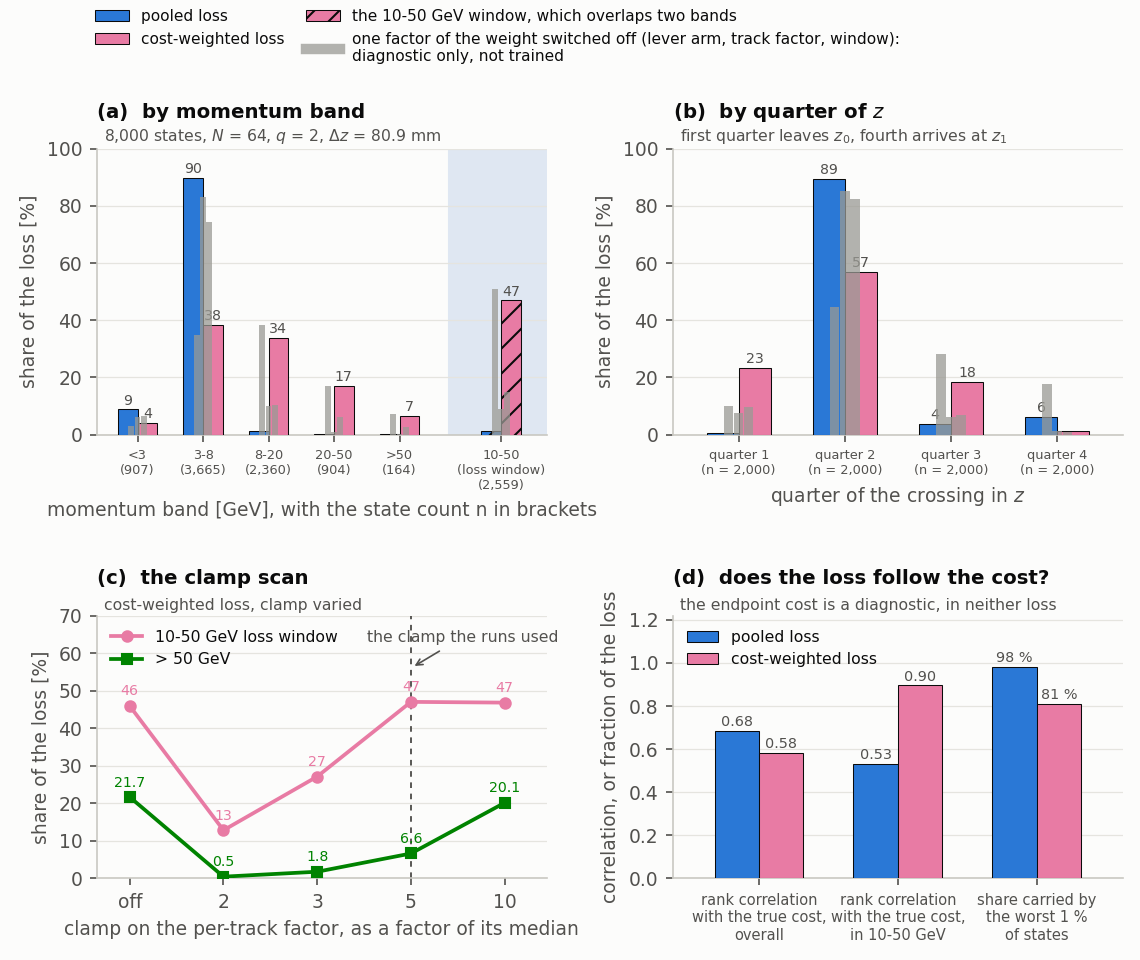
\includegraphics[width=0.95\linewidth]{fig_loss_shares.png}
  \caption{Where each loss spends itself, on the $8{,}000$ pre-flight states
  drawn evenly over the $64$ start planes of the extended pooled-loss
  $N = 64$, $q = 2$, $\Delta z = 80.9\mm$ network. (a) The share of the loss
  carried by each momentum band under the pooled loss and under the
  cost-weighted loss, with the $10$--$50$ GeV window drawn apart on a shaded
  background because it overlaps two of the five bands, and the state count $n$
  printed under each label; the three thin grey bars behind each pair are the
  same shares with the lever arm, the per-track factor or the momentum window
  switched off, which are diagnostics and were never trained. (b) The same by
  quarter of the crossing in $z$, the first quarter being the one that leaves
  $z_0$. (c) The clamp scan of Table~\ref{tab:clamp}: the share carried by the
  window and by the $>50$ GeV band as the clamp on the per-track factor is
  tightened, with the value the runs used marked. (d) How well each objective
  ranks states by what their error actually costs at the endpoint, overall and
  within the window, beside the share of the whole loss carried by the worst
  one per cent of states; the cost is a diagnostic and enters neither
  objective. Source: \texttt{scripts/fig08\_loss\_shares.py}.}
  \label{fig:lossshares}
\end{figure}

% ---------------------------------------------------------------------------
\subsection{Convergence to plateau}
\label{sec:results-plateau}

The comparison that follows is only meaningful if both sides of it had finished
training, so this section applies the plateau rule of
Section~\ref{sec:theory-metrics} to all six runs and states, for each, whether
it had.

\begin{table}[tbp]
  \centering
  \caption{The six runs against the plateau rule of
  Section~\ref{sec:theory-metrics}: the median validation endpoint error of the
  last ten rounds no more than $5$ per cent below the median of the ten before,
  holding at each of the last three rounds. \emph{Flat?} is the verdict at the
  run's last round. \emph{First held} is the earliest round at which the rule
  fired, which for a run that is not flat at its last round means it fired and
  later stopped firing. \emph{Last ten vs previous ten} is the change between
  those two ten-round medians, negative meaning still improving. The
  \emph{validation headline} is the median over the last ten rounds with the
  round-to-round spread beside it, on the $1{,}463$ validation tracks, max
  metric. The three pooled-loss runs are the extended runs, carrying
  respectively $500$, $1{,}000$ and $500$ restarts and $20$, $40$ and $20$
  rounds beyond the snapshot of Table~\ref{tab:grid}. Source:
  \texttt{results/tab\_headline\_pairs.csv} and
  \texttt{results/tab\_extended\_vs\_snapshot.csv}.}
  \label{tab:convergence}
  \footnotesize
  \setlength{\tabcolsep}{5pt}
  \begin{tabular}{llrrcrrl}
    \toprule
    network & loss & rounds & restarts & flat? & first held &
    last ten vs & validation \\
    & & & & & & previous ten & headline [\!\um] \\
    \midrule
    $N = 64$, $q = 2$    & pooled        & $50$ & $1{,}260$ & yes & $38$ & $-4.19$ \% & $126.6 \pm 17.5$ \% \\
    $N = 64$, $q = 2$    & cost-weighted & $40$ & $1{,}000$ & yes & $35$ & $+2.82$ \% & $89.3 \pm 11.7$ \% \\
    $N = 128$, $q = 8$   & pooled        & $63$ & $1{,}599$ & \textbf{no} & $28$ & $-7.24$ \% & $128.7 \pm 12.4$ \% \\
    $N = 128$, $q = 8$   & cost-weighted & $40$ & $1{,}000$ & yes & $35$ & $+0.50$ \% & $107.0 \pm 10.8$ \% \\
    $N = 256$, $q = 16$  & pooled        & $42$ & $1{,}050$ & \textbf{no} & $34$ & $-10.94$ \% & $149.5 \pm \phantom{0}9.8$ \% \\
    $N = 256$, $q = 16$  & cost-weighted & $60$ & $1{,}807$ & yes & $60$ & $+0.55$ \% & $86.4 \pm 25.9$ \% \\
    \bottomrule
  \end{tabular}
\end{table}

Read it this way. All three cost-weighted runs are flat at their last round.
Their ten-round medians moved by $+2.8$, $+0.5$ and $+0.5$ per cent over the
preceding ten, which is to say they moved by nothing, and each fired the rule
several rounds before it was stopped --- at rounds $35$, $35$ and $60$ out of
$40$, $40$ and $60$. Of the three pooled-loss counterparts only one is flat.
The $N = 64$, $q = 2$ run is: it fired at round $38$ of $50$ and its last ten
rounds sit $4.2$ per cent below the ten before, inside the rule's five per cent.
\textbf{The other two are not.} The $N = 128$, $q = 8$ run was still improving
at $7.2$ per cent per ten rounds when it stopped at round $63$, and the
$N = 256$, $q = 16$ run at $10.9$ per cent per ten rounds when it stopped at
round $42$ --- and that is after both had already been extended well past the
18 September snapshot, by $1{,}000$ and $500$ restarts respectively. Both fired
the rule once, at rounds $28$ and $34$, and then resumed falling, which is
exactly the behaviour the rule's one-sidedness is there to catch.

The consequence has to be stated before the comparison and not after it. Two of
the three pooled-loss rows in every later table are \textbf{lower bounds on how
good that network would eventually be}, not converged numbers. If those two runs
were trained to a real plateau their endpoint errors would fall further, and the
margin the cost-weighted loss shows over them at $N = 128$ and $N = 256$ would
shrink by an unknown amount. Extrapolating the observed rate is not a
substitute for running them, and I do not do it. The conclusions of this paper
therefore rest on the $N = 64$, $q = 2$ pair, which is the pre-registered one
and is the only pair in which both sides are flat; the other two pairs are
reported in full, with this caveat attached to every row, and are read as
supporting rather than as independent evidence.

One further number in the table deserves attention because it affects how the
headline should be read. The validation headline carries a round-to-round
spread, and that spread is not small: $17.5$, $11.7$, $12.4$, $10.8$, $9.8$ and
$25.9$ per cent over the six runs. The last of those, the $N = 256$, $q = 16$
cost-weighted run, is the widest in the set, and its plateau verdict rests on a
rule applied to a noisier signal than the others. Any difference between two
runs that is comparable with these numbers is not a difference at all, which is
why the criterion of Section~\ref{sec:theory-metrics} was written as a band to
be cleared rather than as an inequality between two medians.

Figure~\ref{fig:convergence} shows the histories.

\begin{figure}[tbp]
  \centering
  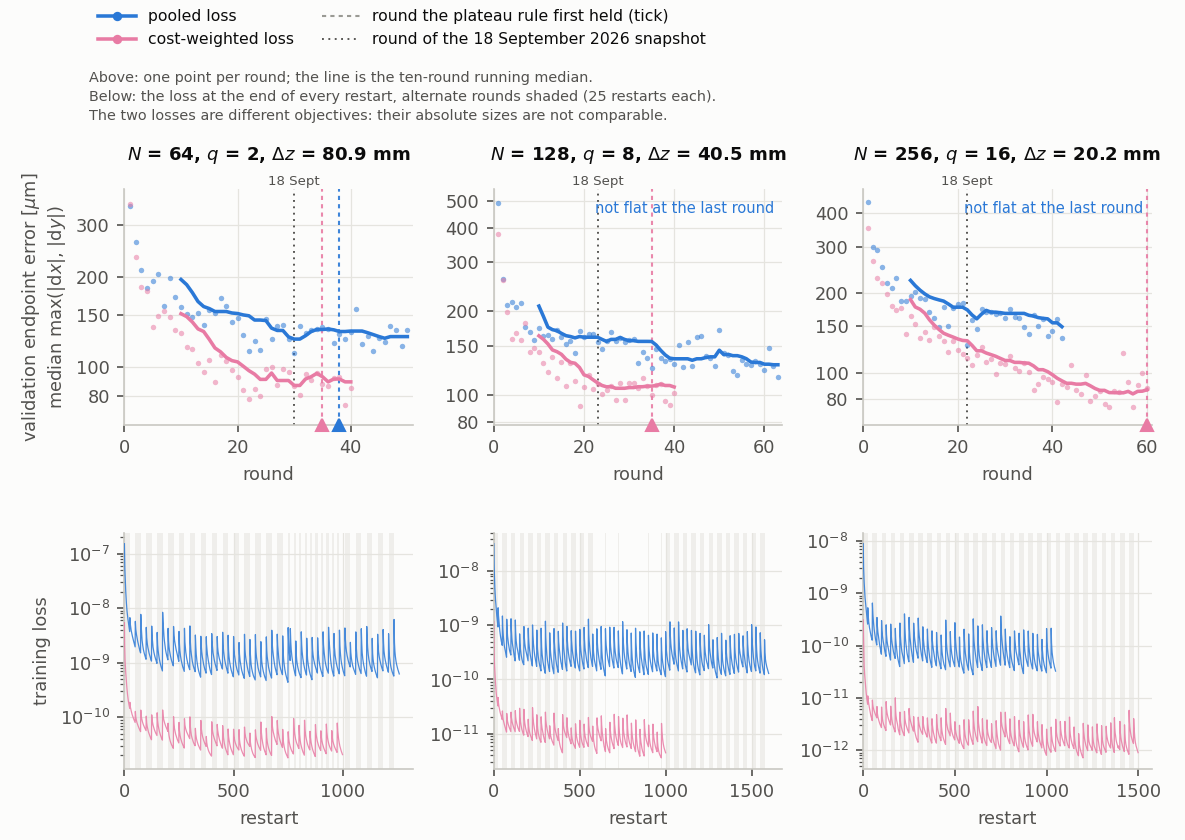
\includegraphics[width=0.95\linewidth]{fig_convergence.png}
  \caption{How the six runs converged, one column per network. Top row: the
  validation endpoint error --- the median over the $1{,}463$ validation tracks
  of $\max(|\Delta x|, |\Delta y|)$ at $z_1$ --- round by round as points, with
  the ten-round running median over them as a line, for the pooled-loss run and
  the cost-weighted-loss run together. On each curve for which the
  plateau rule holds at its last round, a tick marks the round at which the
  rule first held; the two pooled-loss curves that do not satisfy the rule at
  their last round carry no tick and are annotated ``not flat''. The dotted vertical line
  on each pooled-loss curve is the round of the 18 September 2026 snapshot, so
  everything to the right of it is the extension this paper uses. The axis is
  the ordinal round, which is what the tables count. Bottom row: the training
  loss at the end of every restart on a logarithmic axis, with alternate rounds
  shaded so that the round boundaries and the redrawn batch of $32{,}000$
  collocation states at each are visible. The two losses are different
  objectives and their absolute sizes are not comparable; only the shape of
  each curve is. Source: \texttt{scripts/fig09\_convergence.py}.}
  \label{fig:convergence}
\end{figure}

% ---------------------------------------------------------------------------
\subsection{The headline: three networks, two losses}
\label{sec:results-headline}

This is the comparison the paper exists to make: the same network, at the same
three step lengths, trained twice and scored identically, against the criterion
that was fixed before the runs were submitted.

\begin{table}[tbp]
  \centering
  \caption{The headline comparison. Three networks, each trained under the
  pooled loss of Eq.~\eqref{eq:pooled} and under the cost-weighted loss of
  Eq.~\eqref{eq:lossF}, scored on the same $1{,}452$ test tracks against the
  reference at $z_1$. Positions are radial medians in micrometres; the per-step
  slope errors are medians over all steps and all test tracks of the local
  deviation of one application, and are dimensionless. \emph{In window} is the
  $10$--$50$ GeV loss window. \textbf{The pooled-loss runs are the runs extended
  past the 18 September snapshot, and two of the three --- $N = 128$, $q = 8$
  and $N = 256$, $q = 16$ --- were still improving at their last round}
  (Table~\ref{tab:convergence}); their rows are therefore not converged and the
  differences in those two pairs are upper bounds. Source:
  \texttt{results/tab\_headline\_pairs.csv},
  \texttt{results/tab\_reweighted\_runs.csv} and
  \texttt{results/tab\_anatomy.csv}.}
  \label{tab:headline}
  \footnotesize
  \setlength{\tabcolsep}{3pt}
  \begin{tabular}{llrrrrrrr}
    \toprule
    network & loss & median & p95 & $>1\mm$ & in window & $<3$ GeV &
    per-step $t_x$ / $t_y$ & wall \\
    & & [\!\um] & [\!\um] & [\%] & [\!\um] & [\!\um] & [$10^{-7}$] & [h] \\
    \midrule
    $N = 64$, $q = 2$ & pooled        & $145.7$ & $\phantom{0}898$   & $4.41$ & $108.1$ & $353.7$ & $13.0$ / $7.2$ & $31.2$ \\
                      & cost-weighted & $\mathbf{88.8}$  & $1{,}399$ & $7.16$ & $\mathbf{24.8}$  & $615.1$ & $\phantom{0}7.3$ / $9.7$ & $21.6$ \\
    \addlinespace
    $N = 128$, $q = 8$ & pooled        & $122.2$ & $\phantom{0}928$   & $4.41$ & $70.5$ & $333.7$ & $\phantom{0}5.5$ / $3.2$ & $54.7$ \\
                       & cost-weighted & $104.6$ & $1{,}611$ & $9.57$ & $27.3$ & $900.2$ & $\phantom{0}3.8$ / $5.0$ & $32.8$ \\
    \addlinespace
    $N = 256$, $q = 16$ & pooled        & $147.7$ & $1{,}032$ & $5.23$ & $89.6$ & $373.5$ & $\phantom{0}3.0$ / $1.8$ & $63.2$ \\
                        & cost-weighted & $92.2$  & $1{,}230$ & $6.54$ & $34.6$ & $556.7$ & $\phantom{0}1.9$ / $2.4$ & $100.4$ \\
    \bottomrule
  \end{tabular}
\end{table}

Read it this way. Take the pre-registered pair first. Under the pooled loss the
$N = 64$, $q = 2$ network reaches a median endpoint error of $145.7\um$; under
the cost-weighted loss, $88.8\um$. That is a fall of $39.1$ per cent. Inside the
$10$--$50$ GeV window the fall is from $108.1$ to $24.8\um$, a factor $4.37$.
Both of those are improvements, both are large, and neither is the whole story.
Over the same tracks the 95th percentile rises from $898$ to $1{,}399\um$, a
factor $1.56$; the fraction of tracks ending more than a millimetre from the
reference rises from $4.41$ to $7.16$ per cent, from $64$ tracks to $104$; and
the median for tracks below $3$ GeV rises from $353.7$ to $615.1\um$, a factor
$1.74$. The cost-weighted loss made the typical track better, made the window
it was aimed at dramatically better, and made the soft tracks and the tail
worse. That is a trade and not a free improvement, and it is the trade the
objective was designed to make.

The same shape appears at the other two step lengths, with the caveat of
Section~\ref{sec:results-plateau} attached. At $N = 128$, $q = 8$ the median
falls from $122.2$ to $104.6\um$, only $14.4$ per cent, while the window falls
from $70.5$ to $27.3\um$, a factor $2.58$; the p95 rises by a factor $1.74$ and
the sub-$3$ GeV median by a factor $2.70$, the largest degradation anywhere in
the table. At $N = 256$, $q = 16$ the median falls from $147.7$ to $92.2\um$,
$37.6$ per cent, and the window from $89.6$ to $34.6\um$, a factor $2.59$, with
the p95 rising by only a factor $1.19$. The in-window gain is the one consistent
feature: a factor between $2.6$ and $4.4$ at all three step lengths.

The per-step slope errors are worth reading across rather than down. Within each
pair the cost-weighted loss improves the $x$ slope --- the bending plane --- and
worsens the $y$ slope: $13.0$ to $7.3$ and $7.2$ to $9.7$, in units of
$10^{-7}$, at $N = 64$; $5.5$ to $3.8$ and $3.2$ to $5.0$ at $N = 128$;
$3.0$ to $1.9$ and $1.8$ to $2.4$ at $N = 256$. Section~\ref{sec:results-anatomy}
takes that apart. Down the table, both slopes fall by roughly a factor two for
each halving of $\Delta z$, which is what a well-behaved step should do, and the
endpoint medians do not follow them at all;
Section~\ref{sec:results-shortersteps} is about that.

\begin{table}[tbp]
  \centering
  \caption{The same six runs, radial endpoint median per momentum band, with
  the 95th percentile beside it. The five bands partition the test set; the
  $10$--$50$ GeV loss window overlaps two of them and is reported as an extra
  row. $n$ is the number of test tracks in the band. The $>50$ GeV row holds
  $30$ tracks and is read cautiously throughout this paper. The pooled-loss
  rows for $N = 128$, $q = 8$ and $N = 256$, $q = 16$ are not converged
  (Table~\ref{tab:convergence}). Source:
  \texttt{results/tab\_headline\_bands.csv}.}
  \label{tab:headlinebands}
  \footnotesize
  \setlength{\tabcolsep}{4pt}
  \begin{tabular}{lrrrrrrr}
    \toprule
    & & \multicolumn{2}{c}{$N = 64$, $q = 2$} &
        \multicolumn{2}{c}{$N = 128$, $q = 8$} &
        \multicolumn{2}{c}{$N = 256$, $q = 16$} \\
    \cmidrule(lr){3-4}\cmidrule(lr){5-6}\cmidrule(lr){7-8}
    band [GeV] & $n$ & pooled & cost-w. & pooled & cost-w. & pooled & cost-w. \\
    \midrule
    \multicolumn{8}{l}{\emph{median, \um}}\\
    $<3$                    & $164$ & $353.7$ & $615.1$ & $333.7$ & $900.2$ & $373.5$ & $556.7$ \\
    $3$--$8$                & $655$ & $160.4$ & $175.5$ & $153.7$ & $214.1$ & $200.4$ & $177.7$ \\
    $8$--$20$               & $433$ & $86.3$  & $33.4$  & $79.2$  & $43.4$  & $106.5$ & $46.6$  \\
    $20$--$50$              & $170$ & $145.5$ & $16.2$  & $70.2$  & $21.2$  & $78.6$  & $20.2$  \\
    $>50$                   & $30$  & $170.7$ & $22.4$  & $168.0$ & $31.5$  & $216.0$ & $46.6$  \\
    $10$--$50$ (loss window) & $487$ & $108.1$ & $\mathbf{24.8}$ & $70.5$ & $\mathbf{27.3}$ & $89.6$ & $\mathbf{34.6}$ \\
    \midrule
    \multicolumn{8}{l}{\emph{95th percentile, \um}}\\
    $<3$                    & $164$ & $1{,}390$ & $2{,}768$ & $1{,}537$ & $3{,}668$ & $1{,}857$ & $2{,}866$ \\
    $3$--$8$                & $655$ & $1{,}035$ & $1{,}513$ & $1{,}106$ & $1{,}626$ & $1{,}247$ & $1{,}213$ \\
    $8$--$20$               & $433$ & $368$     & $210$     & $362$     & $273$     & $455$     & $246$ \\
    $20$--$50$              & $170$ & $373$     & $64$      & $308$     & $67$      & $301$     & $76$ \\
    $>50$                   & $30$  & $1{,}111$ & $124$     & $521$     & $77$      & $742$     & $111$ \\
    $10$--$50$ (loss window) & $487$ & $353$    & $130$     & $306$     & $158$     & $389$     & $142$ \\
    \bottomrule
  \end{tabular}
\end{table}

Read the band table this way. There is a crossover and it sits between $3$--$8$
and $8$--$20$ GeV. Below it the cost-weighted network is worse in five of the
six comparisons, the exception being $3$--$8$ GeV at $N = 256$, where the
median falls from $200.4$ to $177.7\um$, a reduction of $11.3$ per cent; above it, it is better in all nine. At $N = 64$ the ratios run
$0.58$, $0.91$, $2.59$, $9.01$ and $7.62$ across the five bands from soft to
hard --- that is, $1.7$ times worse below $3$ GeV and nine times better at
$20$--$50$ GeV. At $N = 128$ they run $0.37$, $0.72$, $1.83$, $3.31$, $5.33$,
and at $N = 256$, $0.67$, $1.13$, $2.29$, $3.89$, $4.64$. The $>50$ GeV column
holds only $30$ test tracks and is quoted here for completeness; its medians
move by factors of $5$ to $8$ and a band of that size cannot support a
quantitative claim, so I read it only as agreeing in direction with the
$20$--$50$ GeV band beside it. The 95th percentiles tell the same story more
sharply: above the crossover the tail improves along with the median, by a
factor of up to $5.9$ at $20$--$50$ GeV; below it the tail is where the whole
cost is paid, and at $N = 128$ the sub-$3$ GeV p95 more than doubles, to
$3.67\mm$.

\paragraph{The pre-registered criterion.} Section~\ref{sec:theory-metrics}
fixed what success would have to look like, and the test is as follows. The
first condition was that the $N = 64$, $q = 2$ network's test radial error clear
a $\pm 13$ per cent run-to-run band downward against its pooled-loss
counterpart. It falls by $39.1$ per cent, from $145.7$ to $88.8\um$. The band
was set at $\pm 13$ per cent in advance; the counterpart's actual round-to-round
spread over its last ten rounds, measured after the fact, is $\pm 17.5$ per cent
(Table~\ref{tab:convergence}), and the fall clears that too. \textbf{The first
condition holds}. The second condition was that the median per-step slope error
fall below $1.6\times10^{-6}$. That threshold is the earlier record's
``$0.0016$'', which was quoted in units of $10^{-3}$ of slope and is
$1.6\times10^{-6}$ as a dimensionless number; it was the $N = 64$, $q = 2$
network's own value at the time the criterion was written. The cost-weighted
network reaches $7.34\times10^{-7}$ in $t_x$, a factor $2.18$ below it, and
$2.25\times10^{-7}$ within the loss window. \textbf{The second condition
holds}. For completeness, the extended pooled-loss counterpart has itself since
fallen to $1.30\times10^{-6}$, below the threshold as well, so the second
condition is the weaker of the two: the first is what distinguishes the two
losses.

A partial result had been defined in advance as an in-band improvement without
an overall one, and a null result as nothing clearing the band. Neither applies.
The outcome is the full one, with the pre-registered price attached: the
improvement is real, it is concentrated where the weight was put, and it is
paid for below $3$ GeV and in the tail. Figures~\ref{fig:headline}
and~\ref{fig:tail} show both halves.

\begin{figure}[tbp]
  \centering
  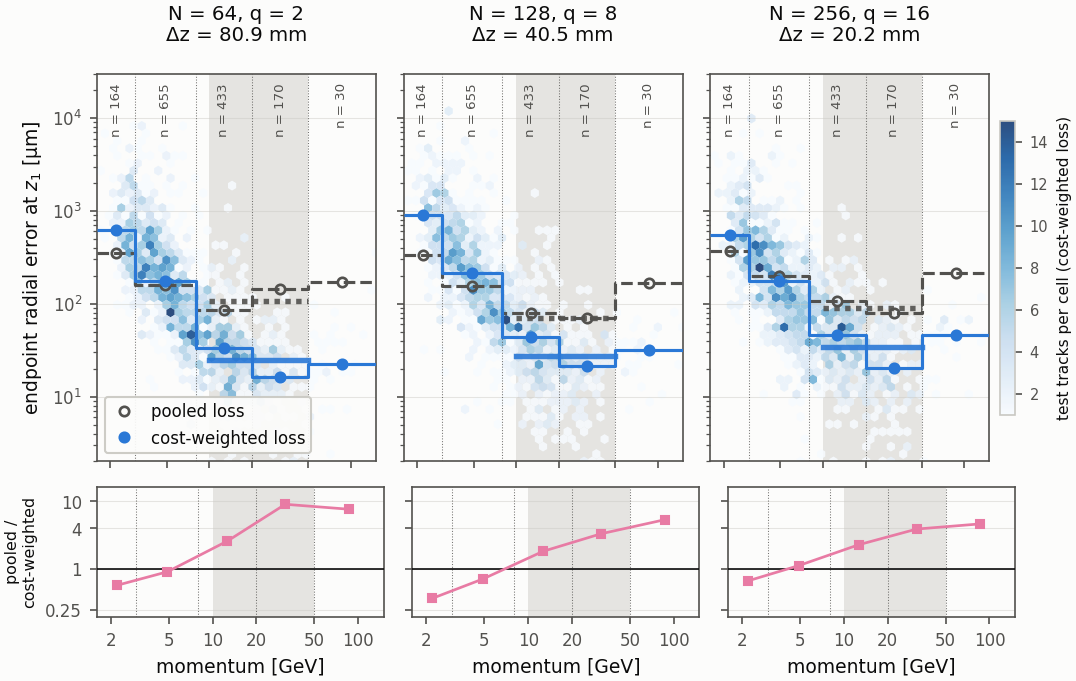
\includegraphics[width=0.95\linewidth]{fig_headline_vs_p.png}
  \caption{The endpoint error against momentum, one column per network. Top
  row: the radial deviation of every test track from the reference at
  $z_1 = 7826.0\mm$, in micrometres on a logarithmic axis, against the track's
  momentum, also logarithmic. The density cloud is the cost-weighted-loss run;
  over it the per-band median of both losses is drawn as a step line with a
  marker at each band centre. The four band edges are thin vertical lines, the
  number of test tracks in each band is printed along the top, and the
  $10$--$50$ GeV loss window is the shaded span. Bottom row: the ratio of the
  two per-band medians, pooled over cost-weighted, on a logarithmic axis with
  unity marked; the curve crosses unity between $3$--$8$ and $8$--$20$ GeV in
  all three networks. No slopes appear in this figure. Source:
  \texttt{scripts/fig10\_headline\_vs\_p.py}.}
  \label{fig:headline}
\end{figure}

\begin{figure}[tbp]
  \centering
  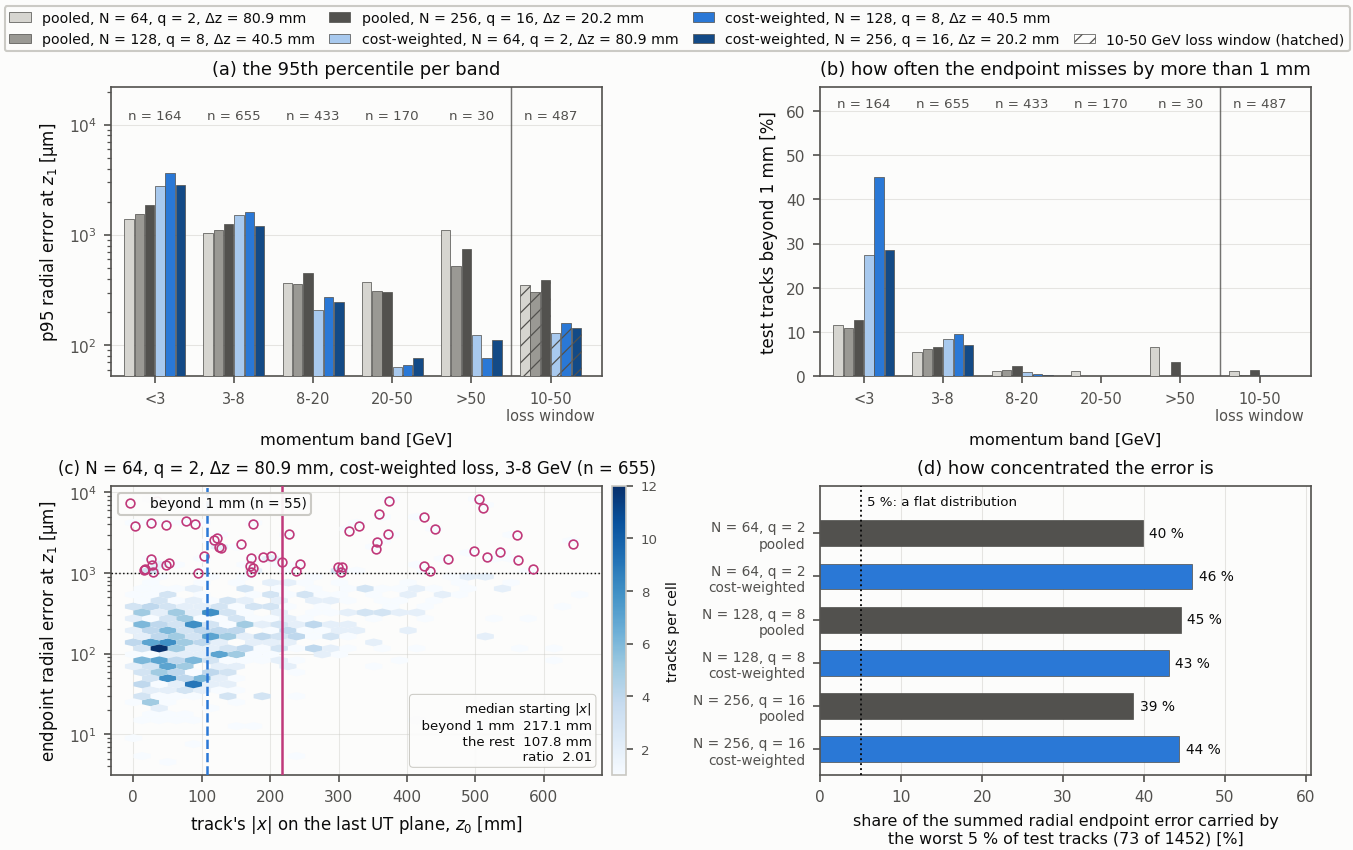
\includegraphics[width=0.95\linewidth]{fig_tail.png}
  \caption{The tail. (a) The 95th percentile of the radial endpoint deviation
  per momentum band for the six runs, logarithmic, with the three pooled-loss
  networks in grey darkening with $N$ beside the same three under the
  cost-weighted loss in blue; the $10$--$50$ GeV loss window is the hatched
  group at the right and $n$ is printed per band. (b) The fraction of test
  tracks whose radial endpoint error exceeds one millimetre, per band, on a
  linear axis. (c) Where the tail tracks start: the radial endpoint error
  against the track's $|x|$ on the last Upstream Tracker plane, for the
  $N = 64$, $q = 2$, $\Delta z = 80.9\mm$ network under the cost-weighted loss
  in the $3$--$8$ GeV band; the tracks beyond one millimetre are circled and the
  median starting $|x|$ of the tail and of the rest are drawn and annotated.
  (d) How concentrated the error is: the share of the summed radial endpoint
  error carried by the worst five per cent of test tracks, $73$ of $1{,}452$,
  for all six runs, against the five per cent a flat distribution would give.
  Source: \texttt{scripts/fig15\_tail.py}.}
  \label{fig:tail}
\end{figure}

% ---------------------------------------------------------------------------
\subsection{Per component, per band}
\label{sec:results-components}

A radial median hides which of the two transverse directions the error is in,
and that turns out to be the most informative thing about this result, so this
section splits the endpoint error into its four predicted components.

\begin{table}[tbp]
  \centering
  \caption{The position components of the endpoint error for the $N = 64$,
  $q = 2$, $\Delta z = 80.9\mm$ network under both losses, per momentum band.
  \emph{med} is the median of $|\Delta|$, \emph{sgn} the median of the signed
  deviation and \emph{hw} the $68$ per cent half-width $(q_{84} - q_{16})/2$ of
  the signed deviation, all in micrometres. A signed median close to the median
  magnitude means a systematic offset; one much smaller means scatter. The
  $>50$ GeV row holds $30$ tracks. Source:
  \texttt{results/tab\_headline\_components.csv}.}
  \label{tab:comppos}
  \footnotesize
  \setlength{\tabcolsep}{3pt}
  \begin{tabular}{lrrrrrrrrrrrrr}
    \toprule
    & & \multicolumn{6}{c}{pooled loss} & \multicolumn{6}{c}{cost-weighted loss} \\
    \cmidrule(lr){3-8}\cmidrule(lr){9-14}
    & & \multicolumn{3}{c}{$\Delta x$} & \multicolumn{3}{c}{$\Delta y$}
      & \multicolumn{3}{c}{$\Delta x$} & \multicolumn{3}{c}{$\Delta y$} \\
    \cmidrule(lr){3-5}\cmidrule(lr){6-8}\cmidrule(lr){9-11}\cmidrule(lr){12-14}
    band [GeV] & $n$ & med & sgn & hw & med & sgn & hw & med & sgn & hw & med & sgn & hw \\
    \midrule
    all        & $1452$ & $110.7$ & $-39.4$ & $164.7$ & $52.3$ & $-15.5$ & $86.4$  & $37.5$  & $-3.6$   & $97.6$  & $55.2$  & $+2.9$   & $139.8$ \\
    $<3$       & $164$  & $249.7$ & $+7.6$  & $382.4$ & $183.4$ & $-25.6$ & $275.3$ & $323.3$ & $+139.1$ & $479.0$ & $393.1$ & $+119.6$ & $725.6$ \\
    $3$--$8$   & $655$  & $118.8$ & $-29.1$ & $192.7$ & $63.5$ & $-10.4$ & $102.7$ & $84.3$  & $-5.6$   & $148.0$ & $118.3$ & $+7.2$   & $233.3$ \\
    $8$--$20$  & $433$  & $62.9$  & $-38.6$ & $90.6$  & $40.8$ & $-18.8$ & $53.3$  & $14.4$  & $-1.6$   & $24.5$  & $24.3$  & $+1.1$   & $41.7$ \\
    $20$--$50$ & $170$  & $134.1$ & $-98.6$ & $135.8$ & $37.5$ & $-27.5$ & $47.2$  & $10.4$  & $-8.0$   & $13.9$  & $6.2$   & $+0.2$   & $12.3$ \\
    $>50$      & $30$   & $145.6$ & $-60.4$ & $236.1$ & $23.9$ & $+3.4$  & $32.7$  & $16.6$  & $-12.6$  & $25.2$  & $10.4$  & $+5.1$   & $14.2$ \\
    $10$--$50$ & $487$  & $86.9$  & $-54.4$ & $105.9$ & $39.6$ & $-22.8$ & $49.5$  & $11.6$  & $-6.3$   & $17.5$  & $13.9$  & $+2.0$   & $24.2$ \\
    \bottomrule
  \end{tabular}
\end{table}

\begin{table}[tbp]
  \centering
  \caption{The slope components of the same endpoint error, same network, same
  bands. $t_x$ and $t_y$ are $\mathrm{d}x/\mathrm{d}z$ and
  $\mathrm{d}y/\mathrm{d}z$ and are dimensionless; every entry is a pure number
  and nothing here is scaled. \emph{med} is the median of $|\Delta|$,
  \emph{sgn} the median of the signed deviation, \emph{hw} the $68$ per cent
  half-width, all $\times 10^{-5}$. Source:
  \texttt{results/tab\_headline\_components.csv}.}
  \label{tab:compslope}
  \footnotesize
  \setlength{\tabcolsep}{3pt}
  \begin{tabular}{lrrrrrrrrrrrrr}
    \toprule
    & & \multicolumn{6}{c}{pooled loss} & \multicolumn{6}{c}{cost-weighted loss} \\
    \cmidrule(lr){3-8}\cmidrule(lr){9-14}
    & & \multicolumn{3}{c}{$\Delta t_x$} & \multicolumn{3}{c}{$\Delta t_y$}
      & \multicolumn{3}{c}{$\Delta t_x$} & \multicolumn{3}{c}{$\Delta t_y$} \\
    \cmidrule(lr){3-5}\cmidrule(lr){6-8}\cmidrule(lr){9-11}\cmidrule(lr){12-14}
    band [GeV] & $n$ & med & sgn & hw & med & sgn & hw & med & sgn & hw & med & sgn & hw \\
    \midrule
    all        & $1452$ & $3.68$ & $-1.62$ & $5.48$  & $2.14$ & $-0.30$ & $3.52$ & $3.23$  & $-1.08$ & $7.65$  & $3.89$  & $+0.79$ & $10.02$ \\
    $<3$       & $164$  & $9.06$ & $-0.61$ & $14.18$ & $5.60$ & $+0.99$ & $8.54$ & $25.39$ & $-1.81$ & $41.40$ & $34.67$ & $+3.54$ & $67.81$ \\
    $3$--$8$   & $655$  & $3.48$ & $-1.50$ & $5.89$  & $2.68$ & $-0.16$ & $4.30$ & $6.98$  & $-3.59$ & $12.20$ & $8.98$  & $+3.00$ & $17.16$ \\
    $8$--$20$  & $433$  & $2.82$ & $-1.66$ & $3.49$  & $1.59$ & $-0.32$ & $2.30$ & $1.37$  & $-0.68$ & $1.88$  & $1.91$  & $+0.74$ & $2.60$ \\
    $20$--$50$ & $170$  & $4.03$ & $-2.99$ & $4.50$  & $1.69$ & $-1.25$ & $1.94$ & $0.85$  & $-0.64$ & $1.10$  & $0.85$  & $+0.19$ & $1.20$ \\
    $>50$      & $30$   & $5.57$ & $-0.11$ & $9.01$  & $1.18$ & $-0.08$ & $1.49$ & $0.99$  & $-0.40$ & $1.62$  & $0.49$  & $+0.30$ & $0.57$ \\
    $10$--$50$ & $487$  & $3.42$ & $-2.08$ & $3.89$  & $1.55$ & $-0.74$ & $2.14$ & $1.06$  & $-0.75$ & $1.35$  & $1.26$  & $+0.43$ & $1.88$ \\
    \bottomrule
  \end{tabular}
\end{table}

Read the two tables together. The whole of the gain is in $x$, and $x$ is the
bending plane: the magnet's field is close to vertical, so it deflects the
particle horizontally, and the correction the surrogate has to reproduce lives
almost entirely in $x$. Over all tracks the median $|\Delta x|$ falls from
$110.7$ to $37.5\um$, a factor $2.95$, while the median $|\Delta y|$ goes from
$52.3$ to $55.2\um$, which is $5.6$ per cent \emph{worse}. Inside the loss
window the two fall together --- $86.9$ to $11.6\um$ in $x$ and $39.6$ to
$13.9\um$ in $y$ --- but the ordering has swapped: under the pooled loss the
$x$ error is $2.2$ times the $y$ error in the window, and under the
cost-weighted loss the $y$ error is the larger of the two by a factor $1.20$.
What limits the reweighted network in its own window is now the non-bending
plane.

The signed medians are the sharper statement. In the window the pooled-loss
network sits at $-54.4\um$ in $x$ against a median magnitude of $86.9$: two
thirds of its typical error is a common offset in one direction, which is a
systematic under-bend and not scatter. The cost-weighted network sits at
$-6.3\um$ against $11.6$. The absolute offset has fallen by a factor $8.7$,
in step with the error itself. I want to be careful about how far that
generalises. As a fraction of the median magnitude the offset is $0.63$ before
and $0.54$ after at $N = 64$, which is barely a change; at $N = 128$ it goes
from $+17.9$ against $53.9\um$ to $+0.15$ against $13.7\um$, a fraction of
$0.33$ falling to $0.011$, and at $N = 256$ from $+30.3$ against $68.9\um$ to
$-2.7$ against $12.3\um$, $0.44$ falling to $0.22$. The sign of the pooled-loss
offset is also not common to the three: it is negative at $N = 64$ and positive
at $N = 128$ and $N = 256$. So the defensible claim is that the cost-weighted
loss reduces the in-window offset in absolute terms in all three pairs and
reduces it relative to the error's own size in two of the three; it is not that
it removes a universal under-bend.

The slope table repeats the position table one derivative down, which is what
Section~\ref{sec:results-anatomy} would lead one to expect. In the window the
median $|\Delta t_x|$ falls from $3.42\times10^{-5}$ to $1.06\times10^{-5}$ and
$|\Delta t_y|$ from $1.55\times10^{-5}$ to $1.26\times10^{-5}$, so again both
improve and again $y$ becomes the larger. Below $3$ GeV both slopes get much
worse, $9.06$ to $25.4$ and $5.60$ to $34.7$ in units of $10^{-5}$, which is the
same trade seen in the positions and is where the soft-track degradation of
Table~\ref{tab:headlinebands} comes from. The $68$ per cent half-widths are
consistently about $1.5$ times the median magnitude throughout, which is what a
roughly symmetric distribution with a modest tail gives, and they move with the
medians rather than independently.

The other two networks behave the same way and are summarised rather than
tabulated in full. At $N = 128$, $q = 8$ the median $|\Delta x|$ over all tracks
falls from $81.7$ to $51.3\um$ and $|\Delta y|$ rises from $59.2$ to
$61.2\um$; in the window $x$ falls from $53.9$ to $13.7\um$ and $y$ from $34.7$
to $16.9\um$. At $N = 256$, $q = 16$ the overall $|\Delta x|$ falls from $103.4$
to $37.6\um$ while $|\Delta y|$ falls only from $69.7$ to $61.3\um$; in the
window $x$ falls from $68.9$ to $12.3\um$ and $y$ from $40.4$ to $27.0\um$. In
all three pairs the $x$ error improves by between $1.6$ and $7.5$ times and the
$y$ error by between $0.95$ and $2.9$, and in all three the cost-weighted
network's in-window error is dominated by $y$. That is a structural statement
about the result and it is the one the discussion returns to.
Figure~\ref{fig:components} draws all six runs and all four components together.

\begin{figure}[tbp]
  \centering
  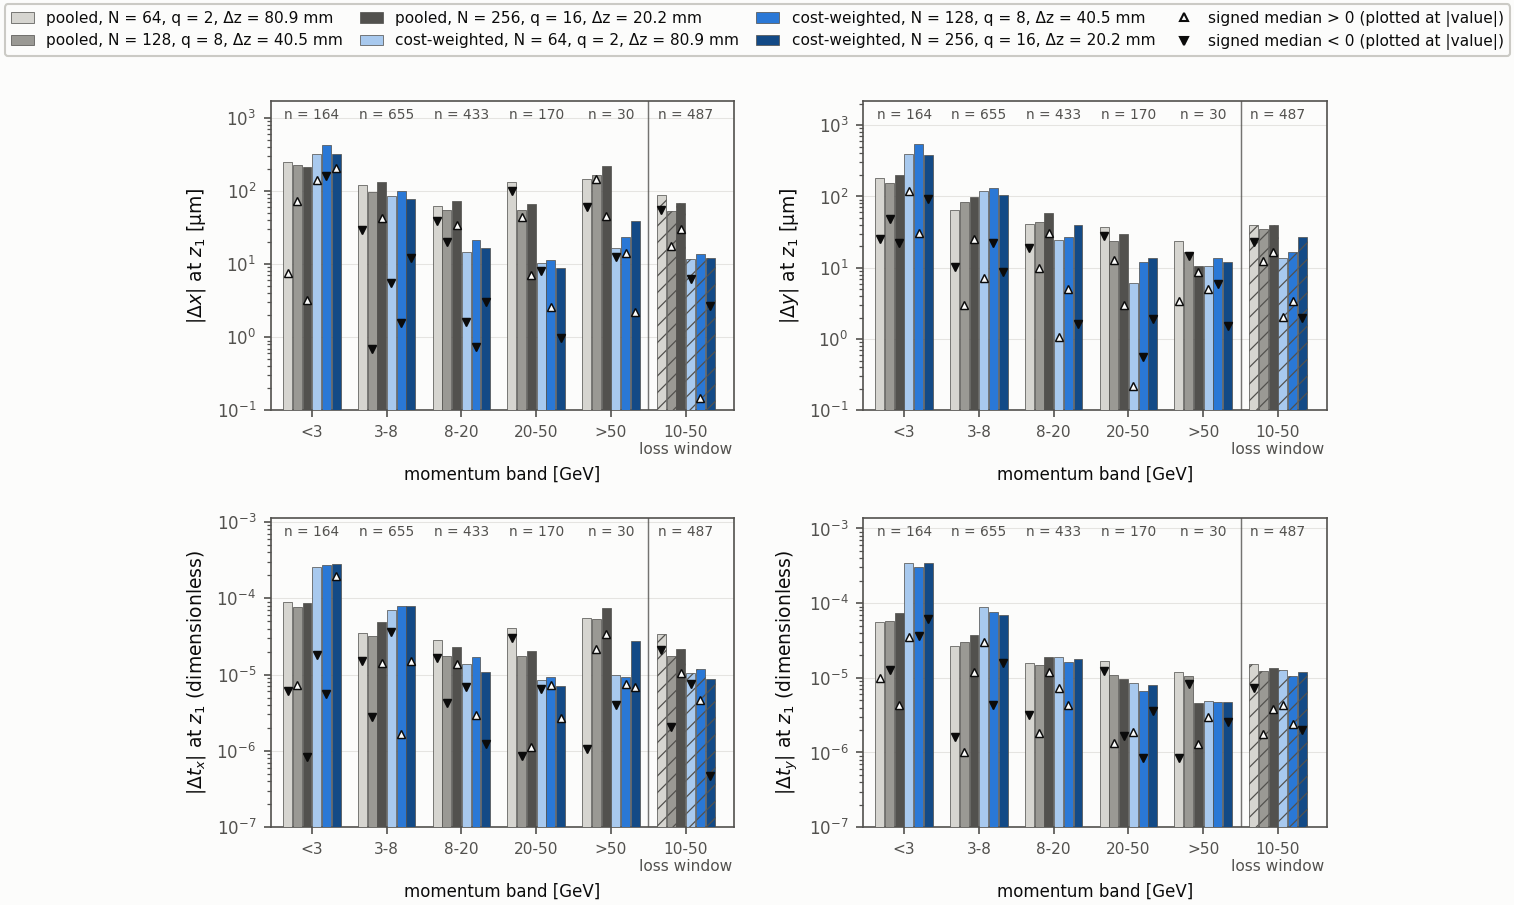
\includegraphics[width=0.98\linewidth]{fig_components_by_band.png}
  \caption{The four state components of the endpoint error at $z_1$, band by
  band, for all six runs: $\Delta x$ and $\Delta y$ in micrometres and the
  dimensionless slope deviations $\Delta t_x$ and $\Delta t_y$, all on
  logarithmic axes so that the slope decades read as scientific notation. In
  each panel the grouped bars give the median $|\text{deviation}|$ of the three
  networks under the pooled loss, in grey darkening with $N$, beside the same
  three under the cost-weighted loss in blue. The five bands partition the test
  set and the $10$--$50$ GeV loss window is the hatched group at the right. The
  number of test tracks is printed above each group. On top of every bar a small
  triangle marks the signed median plotted at the same magnitude, pointing up
  when it is positive and down when it is negative, so that the size of the
  systematic part can be compared with the size of the error directly. Source:
  \texttt{scripts/fig11\_components\_by\_band.py}.}
  \label{fig:components}
\end{figure}

% ---------------------------------------------------------------------------
\subsection{Around 5 GeV}
\label{sec:results-5gev}

The region around $5$ GeV was asked for specifically, it sits below the
crossover of Section~\ref{sec:results-headline}, and it is where the
cost-weighted loss is paying rather than earning, so it is worth a section of
its own rather than a row in a band table.

\begin{table}[tbp]
  \centering
  \caption{The $N = 64$, $q = 2$, $\Delta z = 80.9\mm$ network under both losses
  in the $3$--$8$ GeV band and in the $4$--$6$ GeV band, per component. Position
  entries are micrometres; slope entries are dimensionless and are quoted
  $\times 10^{-5}$. \emph{sgn} is the median of the signed deviation,
  \emph{hw68} the $68$ per cent half-width of it, \emph{RMS} the root mean
  square of it and \emph{med} the median of its magnitude. The RMS is quoted
  beside the half-width because the size of the disagreement between them is
  itself the statement about the tail. Source:
  \texttt{results/tab\_near\_5gev.csv}.}
  \label{tab:near5}
  \footnotesize
  \setlength{\tabcolsep}{5pt}
  \begin{tabular}{llrrrrrr}
    \toprule
    band & loss & component & $n$ & sgn & hw68 & RMS & med \\
    \midrule
    $3$--$8$ GeV & pooled        & $\Delta x$ [\!\um]      & $655$ & $-29.1$ & $192.7$ & $708.2$ & $118.8$ \\
                 &               & $\Delta y$ [\!\um]      & $655$ & $-10.4$ & $102.7$ & $739.8$ & $63.5$ \\
                 &               & $\Delta t_x$ [$10^{-5}$] & $655$ & $-1.50$ & $5.89$  & $20.75$ & $3.48$ \\
                 &               & $\Delta t_y$ [$10^{-5}$] & $655$ & $-0.16$ & $4.30$  & $25.07$ & $2.68$ \\
    \addlinespace
                 & cost-weighted & $\Delta x$ [\!\um]      & $655$ & $-5.6$  & $148.0$ & $634.9$ & $84.3$ \\
                 &               & $\Delta y$ [\!\um]      & $655$ & $+7.2$  & $233.3$ & $716.0$ & $118.3$ \\
                 &               & $\Delta t_x$ [$10^{-5}$] & $655$ & $-3.59$ & $12.20$ & $32.65$ & $6.98$ \\
                 &               & $\Delta t_y$ [$10^{-5}$] & $655$ & $+3.00$ & $17.16$ & $52.08$ & $8.98$ \\
    \midrule
    $4$--$6$ GeV & pooled        & $\Delta x$ [\!\um]      & $286$ & $-35.5$ & $203.4$ & $426.1$ & $125.1$ \\
                 &               & $\Delta y$ [\!\um]      & $286$ & $-9.2$  & $96.6$  & $518.2$ & $64.0$ \\
                 &               & $\Delta t_x$ [$10^{-5}$] & $286$ & $-2.02$ & $5.48$  & $13.09$ & $3.55$ \\
                 &               & $\Delta t_y$ [$10^{-5}$] & $286$ & $-0.29$ & $3.97$  & $21.65$ & $2.66$ \\
    \addlinespace
                 & cost-weighted & $\Delta x$ [\!\um]      & $286$ & $-26.5$ & $146.2$ & $618.1$ & $92.8$ \\
                 &               & $\Delta y$ [\!\um]      & $286$ & $+28.1$ & $223.3$ & $425.4$ & $130.0$ \\
                 &               & $\Delta t_x$ [$10^{-5}$] & $286$ & $-5.36$ & $10.27$ & $28.37$ & $7.76$ \\
                 &               & $\Delta t_y$ [$10^{-5}$] & $286$ & $+3.49$ & $16.11$ & $32.86$ & $9.55$ \\
    \bottomrule
  \end{tabular}
\end{table}

\begin{table}[tbp]
  \centering
  \caption{The same two bands summarised, and where the tail tracks start.
  \emph{radial median} and \emph{p95} are of $\sqrt{\Delta x^2 + \Delta y^2}$ at
  $z_1$; \emph{beyond $1\mm$} counts the tracks in the band whose radial
  endpoint error exceeds one millimetre; the last three columns are the median
  $|x|$ of those tracks on the last Upstream Tracker plane $z_0$, the same for
  the rest of the band, and their ratio. Source:
  \texttt{results/tab\_near\_5gev.csv}.}
  \label{tab:near5tail}
  \footnotesize
  \setlength{\tabcolsep}{5pt}
  \begin{tabular}{llrrrrrrr}
    \toprule
    band & loss & $n$ & radial med. & p95 & beyond & start $|x|$ & start $|x|$ & ratio \\
    & & & [\!\um] & [\!\um] & $1\mm$ & tail [\!\mm] & rest [\!\mm] & \\
    \midrule
    $3$--$8$ GeV & pooled        & $655$ & $160.4$ & $1{,}035$ & $36$ & $159.6$ & $109.6$ & $1.46$ \\
                 & cost-weighted & $655$ & $175.5$ & $1{,}513$ & $55$ & $217.1$ & $107.8$ & $2.01$ \\
    $4$--$6$ GeV & pooled        & $286$ & $159.6$ & $\phantom{0}890$ & $14$ & $160.8$ & $115.6$ & $1.39$ \\
                 & cost-weighted & $286$ & $187.1$ & $1{,}106$ & $17$ & $188.8$ & $113.6$ & $1.66$ \\
    \bottomrule
  \end{tabular}
\end{table}

Read it this way. In the $4$--$6$ GeV band the honest single number for the core
of the distribution is the $68$ per cent half-width, not the median magnitude
and certainly not the RMS. Under the cost-weighted loss the half-width in $x$ is
$146\um$ and the RMS is $618\um$, a factor $4.2$ apart, and the reason is
visible in Table~\ref{tab:near5tail}: $17$ of the $286$ tracks end more than a
millimetre away and those few set the RMS entirely. Under the pooled loss the
same two numbers are $203$ and $426\um$, a factor $2.1$ apart with $14$ tracks
beyond a millimetre. The half-width in $x$ is therefore the one component where
the cost-weighted network is better in this band, $146$ against $203\um$, and
it is better because the reweighting did reach down this far in the bending
plane. Everything else here is worse.

The degradation is concentrated in $y$ and it is a shift, not a widening only.
In the $4$--$6$ GeV band the signed median in $y$ goes from $-9.2\um$ under the
pooled loss to $+28.1\um$ under the cost-weighted one, and the half-width from
$96.6$ to $223.3\um$: the distribution has both moved and more than doubled in
width. The same happens in $t_y$, where the signed median goes from
$-2.9\times10^{-6}$ to $+3.5\times10^{-5}$ and the half-width from
$3.97\times10^{-5}$ to $1.61\times10^{-4}$. In the wider $3$--$8$ GeV band the
pattern is identical with slightly smaller numbers. Whatever the reweighting
bought in the window, it took the soft tracks' vertical plane with it, and it
took it by a factor four in the slope's half-width.

The tail columns say something the momentum bands cannot. The tracks that end
beyond a millimetre are not randomly placed: in the $3$--$8$ GeV band under the
cost-weighted loss their median starting $|x|$ on the last Upstream Tracker
plane is $217.1\mm$ against $107.8\mm$ for the rest of the band, a ratio of
$2.01$; under the pooled loss the same ratio is $1.46$, and in the narrower
$4$--$6$ GeV band the ratios are $1.66$ and $1.39$. The tail is made of soft
tracks that start far from the beam line, and it becomes more so under the
cost-weighted loss. A momentum window cannot address that, because the
distinguishing variable is not momentum. Panel (c) of Figure~\ref{fig:tail}
draws it, and Figure~\ref{fig:signed3to8} shows the full signed distributions
these numbers summarise.

\begin{figure}[tbp]
  \centering
  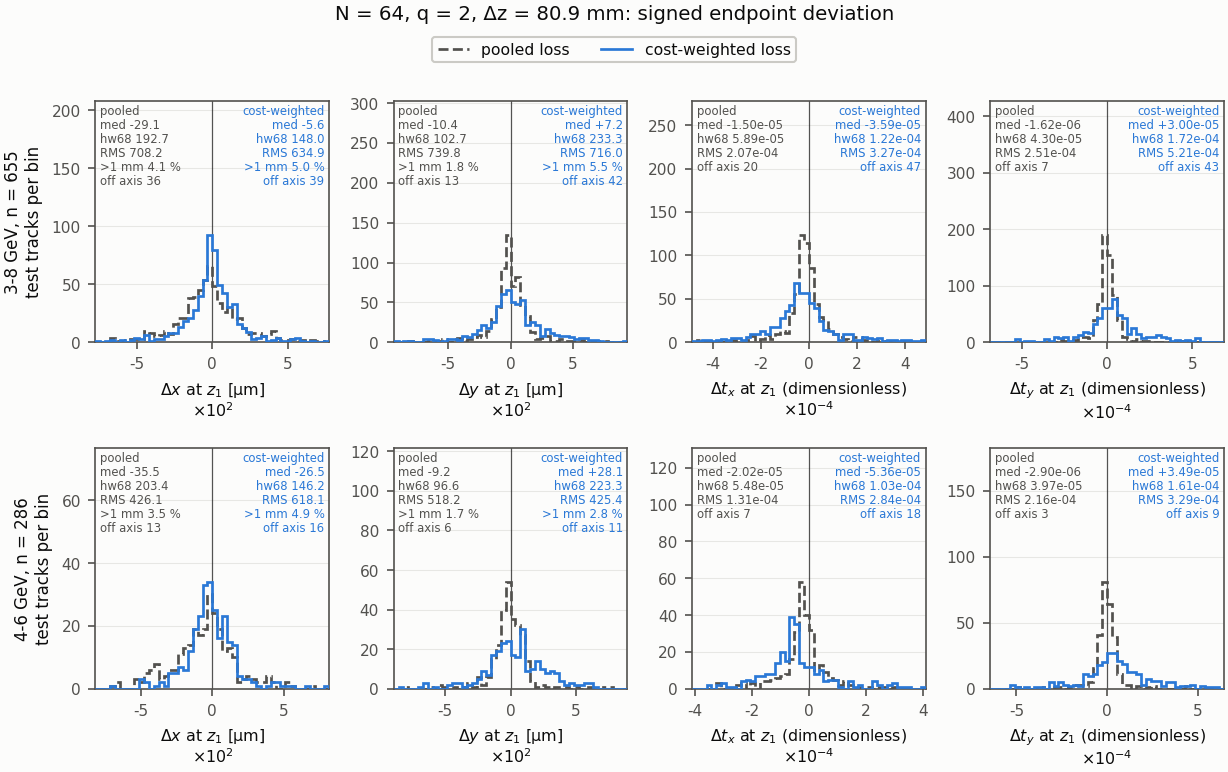
\includegraphics[width=0.95\linewidth]{fig_signed_3to8.png}
  \caption{The signed endpoint deviation of the $N = 64$, $q = 2$,
  $\Delta z = 80.9\mm$ network from the reference at $z_1$, under both losses,
  as step histograms on a common binning. The four columns are $\Delta x$ and
  $\Delta y$ in micrometres and the dimensionless $\Delta t_x$ and $\Delta t_y$,
  whose axes therefore read in scientific notation. Top row: the $3$--$8$ GeV
  band, $n = 655$. Bottom row: the $4$--$6$ GeV band, $n = 286$. Each panel
  annotates, for both losses, the signed median, the $68$ per cent half-width
  and the RMS; the two position columns also print the fraction of tracks whose
  deviation in that component exceeds one millimetre, and every panel prints
  how many tracks fall outside the drawn range, since the bin range is finite.
  Source: \texttt{scripts/fig12\_signed\_3to8.py}.}
  \label{fig:signed3to8}
\end{figure}

% ---------------------------------------------------------------------------
\subsection{What the remaining error is made of}
\label{sec:results-anatomy}

Everything so far describes the error at the far side of the magnet. This
section asks where it came from: whether the endpoint error is accumulated
per-step error and nothing else, how much the individual steps agree with one
another, and which plane carries what is left.

The measurement is made by comparing each step's output with a reference
integration started from the same state that step was given, over the same
$\Delta z$, so that the quantity is the local error of one application in the
middle of a chain rather than a difference from the true trajectory.

\begin{table}[tbp]
  \centering
  \caption{The per-step error of all six runs. Each step's output is compared
  with a reference integration started from the same state the network was
  given, over the same $\Delta z$; the entries are medians over all $N$ steps
  and all $1{,}452$ test tracks. Slopes are dimensionless and are quoted
  $\times 10^{-7}$; positions are micrometres. \emph{radial} is the radial
  per-step position error. The three momentum columns restrict the same
  statistic to tracks in that band. Source: \texttt{results/tab\_anatomy.csv}.}
  \label{tab:anatomysteps}
  \footnotesize
  \setlength{\tabcolsep}{4pt}
  \begin{tabular}{llrrrrrrrr}
    \toprule
    & & \multicolumn{3}{c}{all tracks} & \multicolumn{2}{c}{$3$--$8$ GeV}
      & \multicolumn{2}{c}{$8$--$20$ GeV} & \multicolumn{1}{c}{$10$--$50$} \\
    \cmidrule(lr){3-5}\cmidrule(lr){6-7}\cmidrule(lr){8-9}\cmidrule(lr){10-10}
    network & loss & $|\Delta t_x|$ & $|\Delta t_y|$ & radial
      & $|\Delta t_x|$ & $|\Delta t_y|$ & $|\Delta t_x|$ & $|\Delta t_y|$
      & $|\Delta t_x|$ \\
    & & \multicolumn{2}{c}{[$10^{-7}$]} & [\!\um]
      & \multicolumn{2}{c}{[$10^{-7}$]} & \multicolumn{2}{c}{[$10^{-7}$]}
      & [$10^{-7}$] \\
    \midrule
    $N = 64$, $q = 2$   & pooled        & $13.02$ & $7.16$ & $0.333$ & $14.94$ & $9.97$  & $8.56$ & $4.93$ & $9.49$ \\
                        & cost-weighted & $7.34$  & $9.74$ & $0.433$ & $14.70$ & $21.79$ & $2.96$ & $4.24$ & $2.25$ \\
    \addlinespace
    $N = 128$, $q = 8$  & pooled        & $5.49$  & $3.15$ & $0.172$ & $6.69$  & $4.85$  & $3.41$ & $1.98$ & $3.65$ \\
                        & cost-weighted & $3.77$  & $4.98$ & $0.221$ & $7.64$  & $10.76$ & $1.55$ & $2.24$ & $1.18$ \\
    \addlinespace
    $N = 256$, $q = 16$ & pooled        & $2.99$  & $1.83$ & $0.089$ & $3.65$  & $2.79$  & $1.83$ & $1.23$ & $1.82$ \\
                        & cost-weighted & $1.87$  & $2.38$ & $0.058$ & $3.63$  & $4.94$  & $0.73$ & $1.20$ & $0.57$ \\
    \bottomrule
  \end{tabular}
\end{table}

\begin{table}[tbp]
  \centering
  \caption{How the per-step errors accumulate. \emph{$x$ part} and \emph{$y$
  part} are the medians of $|\Delta x|$ and $|\Delta y|$ at $z_1$, repeated
  here so that the two planes can be compared against the coherences.
  \emph{coherence} is, per track, the magnitude of the sum of the per-step slope
  errors divided by the sum of their magnitudes, with the value
  $1/\sqrt{N}$ that independent steps would give in the column beside it.
  \emph{explained} is the ratio of the lever-arm model of
  Section~\ref{sec:theory-metrics} --- each step's own position error plus its
  slope error times the distance it still has to travel --- to the measured
  radial endpoint error, once with both slopes and once with the $x$ slope
  alone. Source: \texttt{results/tab\_anatomy.csv}.}
  \label{tab:anatomyend}
  \footnotesize
  \setlength{\tabcolsep}{3pt}
  \begin{tabular}{llrrrrrrr}
    \toprule
    & & $x$ part & $y$ part & coherence & coherence & independent
      & explained & explained \\
    network & loss & [\!\um] & [\!\um] & $t_x$ & $t_y$ & steps
      & both slopes & $x$ slope only \\
    \midrule
    $N = 64$, $q = 2$   & pooled        & $107.7$ & $51.9$ & $0.357$ & $0.397$ & $0.125$  & $0.984$ & $0.733$ \\
                        & cost-weighted & $36.4$  & $54.8$ & $0.491$ & $0.518$ & $0.125$  & $0.977$ & $0.377$ \\
    \addlinespace
    $N = 128$, $q = 8$  & pooled        & $79.0$  & $59.1$ & $0.312$ & $0.432$ & $0.0884$ & $0.983$ & $0.634$ \\
                        & cost-weighted & $52.4$  & $59.9$ & $0.527$ & $0.459$ & $0.0884$ & $0.989$ & $0.448$ \\
    \addlinespace
    $N = 256$, $q = 16$ & pooled        & $98.9$  & $69.3$ & $0.411$ & $0.453$ & $0.0625$ & $0.989$ & $0.673$ \\
                        & cost-weighted & $36.7$  & $61.6$ & $0.454$ & $0.474$ & $0.0625$ & $0.994$ & $0.363$ \\
    \bottomrule
  \end{tabular}
\end{table}

Read it this way, and start with the last two columns of
Table~\ref{tab:anatomyend}, because they license everything else. Modelling the
endpoint error as the sum over steps of each step's own position error plus that
step's slope error multiplied by the distance it still has to travel reproduces
the measured radial endpoint error to between $97.7$ and $99.4$ per cent in all
six runs. The decomposition is complete. The endpoint error of a chained network
is accumulated per-step error carried by the lever arm and there is nothing else
in it --- no separate effect of feeding the network its own output, no
instability, nothing that is not already in the per-step numbers. That is a
strong statement and it is measured rather than assumed, and it is what makes
the lever arm the right variable to weight by.

Next, the per-step slopes. In the loss window the cost-weighted network's $x$
slope error is $2.25\times10^{-7}$ against the pooled network's
$9.49\times10^{-7}$, a factor $4.21$; at $N = 128$ the same comparison is
$1.18$ against $3.65$, a factor $3.08$, and at $N = 256$, $0.57$ against $1.82$,
a factor $3.21$. Over all tracks the improvement is smaller, a factor $1.77$,
$1.46$ and $1.60$, because the soft tracks that dominate an unweighted median
were deliberately de-weighted. And in $t_y$ the cost-weighted network is
\emph{worse} over all tracks in all three pairs --- $9.74$ against $7.16$,
$4.98$ against $3.15$, $2.38$ against $1.83$, in units of $10^{-7}$ --- while
being better in the $8$--$20$ GeV band. The $3$--$8$ GeV columns show where that
comes from: there the cost-weighted $t_y$ error is $2.2$, $2.2$ and $1.8$ times
the pooled one. The $y$ degradation of Section~\ref{sec:results-components} is
already present at the level of a single step.

Now the coherences, which explain why the endpoint did not improve as much as
the steps did. If the $N$ steps of a chain erred independently the magnitude of
the sum of their slope errors would be about $1/\sqrt{N}$ of the sum of their
magnitudes --- $0.125$ at $N = 64$, $0.0884$ at $N = 128$, $0.0625$ at
$N = 256$. The measured values are between $0.31$ and $0.53$, so the steps are
between $2.9$ and $7.6$ times more aligned than chance in every run. The steps
are not making independent mistakes; they are making the same mistake
repeatedly, which is what one should expect of a single deterministic map
applied to a smoothly varying sequence of states. Worse, the cost-weighted
networks are \emph{more} coherent than their counterparts in all six of the
matched comparisons: $0.491$ and $0.518$ against $0.357$ and $0.397$ at $N = 64$,
$0.527$ and $0.459$ against $0.312$ and $0.432$ at $N = 128$, $0.454$ and
$0.474$ against $0.411$ and $0.453$ at $N = 256$. Smaller per-step errors that
all point the same way accumulate as efficiently as larger random ones would.
That is the mechanism by which a factor $4.2$ in the in-window per-step slope
became a factor $4.4$ in the in-window endpoint, while a factor $1.8$ in the
overall per-step $x$ slope became a factor $1.6$ in the overall endpoint, and it
is the clearest single reason why shortening the step does not help as much as
it ought to.

Finally, the two plane columns and the $x$-slope-only model. Under the pooled
loss the $x$ part of the endpoint error is larger than the $y$ part in all three
networks --- $107.7$ against $51.9$, $79.0$ against $59.1$, $98.9$ against
$69.3\um$ --- and a decomposition using the $x$ slope alone recovers $63$ to
$73$ per cent of the endpoint error. Under the cost-weighted loss the $x$ part
is the smaller in two of the three --- $36.4$ against $54.8$ and $36.7$ against
$61.6\um$, with $N = 128$ close to equal at $52.4$ against $59.9$ --- and the
$x$-slope-only model recovers only $36$ to $45$ per cent. A one-sided
decomposition was adequate for the pooled-loss networks and is not adequate for
the reweighted ones, because what limits them has moved into the other plane.
Figure~\ref{fig:anatomy} shows the step-by-step measurement for the
pre-registered pair.

\begin{figure}[tbp]
  \centering
  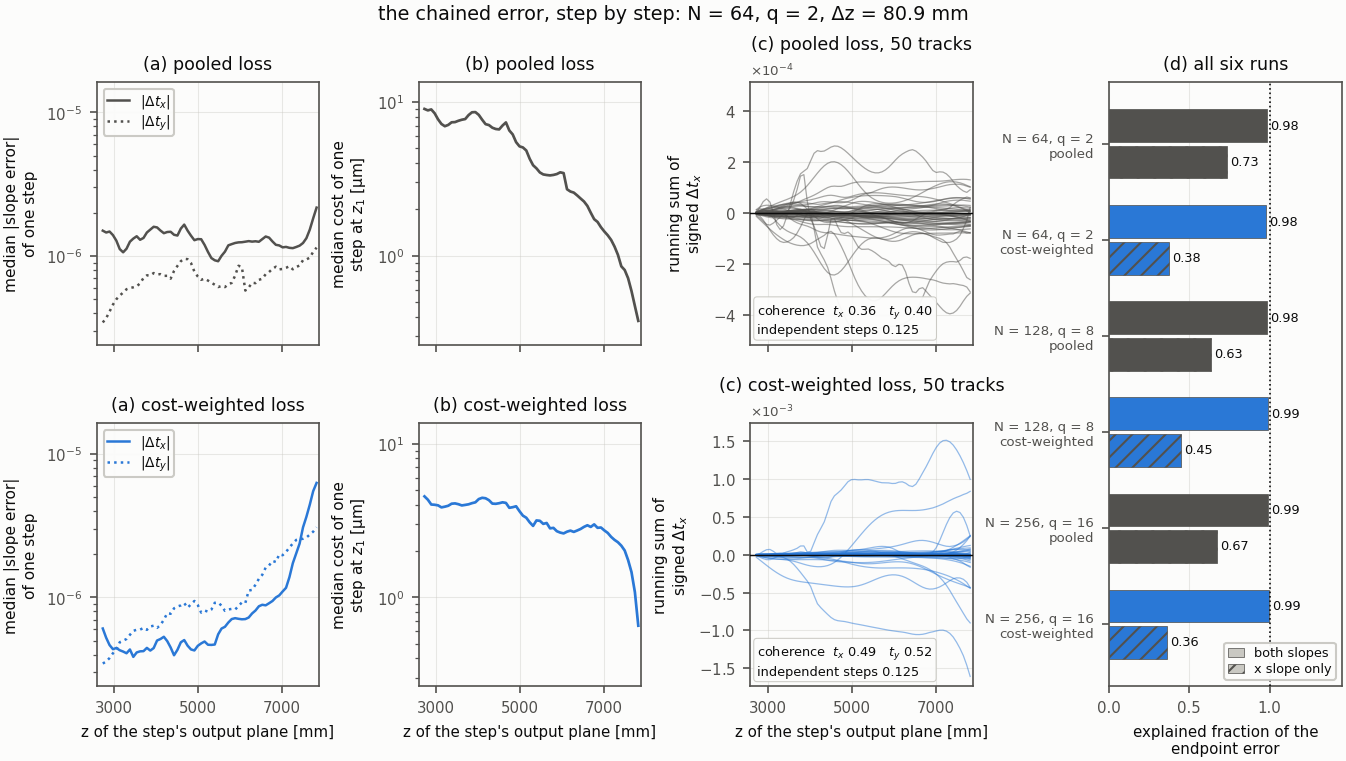
\includegraphics[width=0.97\linewidth]{fig_anatomy.png}
  \caption{The anatomy of the chained error for the two $N = 64$, $q = 2$,
  $\Delta z = 80.9\mm$ networks, the pooled loss on the top row and the
  cost-weighted loss on the bottom. Each step's output is compared with a
  reference integration started from the same state the network was given, over
  the same step. (a) The median $|\Delta t_x|$ and $|\Delta t_y|$ of a single
  step against the $z$ of that step's output plane, dimensionless on a
  logarithmic axis. (b) What each step costs at the endpoint: the median over
  test tracks of that step's position error plus its slope error times the
  distance still to run, in micrometres --- an early step is expensive because
  its slope error is carried a long way. (c) The running sum of the signed
  per-step slope error along the track for $50$ test tracks; the lines drift in
  one direction rather than wandering, which is what the coherence annotated in
  the panel measures, quoted against the $0.125$ that independent steps would
  give. The two rows carry different vertical scales because the drifts differ
  by about a factor four. (d) The explained fraction of the endpoint error for all
  six runs, with both slopes and with the $x$ slope alone. Source:
  \texttt{scripts/fig14\_anatomy.py}.}
  \label{fig:anatomy}
\end{figure}

% ---------------------------------------------------------------------------
\subsection{Shorter steps}
\label{sec:results-shortersteps}

The design in this paper has a free parameter that the first paper did not
have --- how finely to cut the crossing --- and the obvious expectation is that
a shorter step is an easier problem and should give a better crossing; this
section measures that and finds it is not so.

\begin{table}[tbp]
  \centering
  \caption{What shortening the step buys. \emph{per-step radial} and
  \emph{per-step $|\Delta t_x|$} are the local errors of one application of the
  network in the middle of its own chain, medians over all steps and test
  tracks. \emph{single step} is one application started from a reference state
  on an interior plane, median over all planes and tracks; it agrees with the
  per-step radial column to the digits shown, although the two are computed
  from different starting states. \emph{endpoint} and \emph{in window} are the
  radial medians of the full $N$-application chain, repeated from
  Table~\ref{tab:headline}. \emph{chain / step} is the last column of the
  reference divided by the single-step column. Source:
  \texttt{results/tab\_anatomy.csv}, \texttt{results/tab\_along\_z.csv} and
  \texttt{results/tab\_single\_step\_vs\_z.csv}.}
  \label{tab:steps}
  \footnotesize
  \setlength{\tabcolsep}{5pt}
  \begin{tabular}{llrrrrrr}
    \toprule
    network & loss & $\Delta z$ & per-step & per-step & single step &
    endpoint & in window \\
    & & [\!\mm] & radial [\!\um] & $|\Delta t_x|$ & [\!\um] & [\!\um] & [\!\um] \\
    \midrule
    $N = 64$, $q = 2$   & pooled        & $80.90$ & $0.333$ & $1.30\times10^{-6}$ & $0.333$ & $145.7$ & $108.1$ \\
                        & cost-weighted & $80.90$ & $0.433$ & $7.34\times10^{-7}$ & $0.433$ & $88.8$  & $24.8$ \\
    \addlinespace
    $N = 128$, $q = 8$  & pooled        & $40.45$ & $0.172$ & $5.49\times10^{-7}$ & $0.172$ & $122.2$ & $70.5$ \\
                        & cost-weighted & $40.45$ & $0.221$ & $3.77\times10^{-7}$ & $0.221$ & $104.6$ & $27.3$ \\
    \addlinespace
    $N = 256$, $q = 16$ & pooled        & $20.23$ & $0.089$ & $2.99\times10^{-7}$ & $0.089$ & $147.7$ & $89.6$ \\
                        & cost-weighted & $20.23$ & $0.058$ & $1.87\times10^{-7}$ & $0.058$ & $92.2$  & $34.6$ \\
    \bottomrule
  \end{tabular}
\end{table}

Read it this way. Halving the step halves the per-step error, near enough. Under
the pooled loss the per-step radial error goes $0.333 \to 0.172 \to
0.089\um$, ratios of $1.93$ and $1.93$ against the $2.00$ that exact
proportionality to $\Delta z$ would give; the per-step $x$ slope error goes
$1.30 \to 0.549 \to 0.299$ in units of $10^{-6}$, ratios of $2.37$ and $1.84$.
Under the cost-weighted loss the slope goes $7.34 \to 3.77 \to 1.87$ in units of
$10^{-7}$, ratios of $1.95$ and $2.02$, which is as close to proportional as one
could ask. Each network is doing its own job better as the job gets easier.

The endpoint does not follow. Under the pooled loss it goes $145.7 \to 122.2
\to 147.7\um$ and under the cost-weighted loss $88.8 \to 104.6 \to 92.2\um$:
neither sequence is monotone and neither moves by more than a factor $1.21$
across a factor four in step length. Inside the loss window it is worse than
that --- the cost-weighted sequence is $24.8 \to 27.3 \to 34.6\um$, which gets
steadily \emph{worse} as the step shortens, so the network with the smallest
per-step error has the largest in-window endpoint error of the three. The
arithmetic is not mysterious: halving the step halves each step's error and
doubles the number of steps, so a perfectly incoherent chain would improve only
as $\sqrt{\Delta z}$ and a perfectly coherent one would not improve at all. The
coherences of Table~\ref{tab:anatomyend} are between $0.31$ and $0.53$ rather
than at their independent values of $0.13$, $0.088$ and $0.063$, which puts the
chains much closer to the coherent limit than to the incoherent one, and the
measured endpoints are flat, as that limit says they should be.

The ratio of the two errors makes the same point in one number. The chain's
endpoint error is $438$ times its own single-step error at $N = 64$ under the
pooled loss and $205$ times under the cost-weighted one; $710$ and $474$ times
at $N = 128$; and $1{,}653$ and $1{,}587$ times at $N = 256$. A chain of $N$
independent steps would show roughly $\sqrt{N}$, which is $8$, $11$ and $16$,
and a chain in which every step's slope error is carried the full remaining
length would show something of order $N$ times the lever arm in units of the
step --- which is where these numbers live. Figure~\ref{fig:alongz} puts the two
measurements side by side on a common axis, and the gap between the panels is
the whole of this section.

The practical conclusion is that shortening the step is not the lever. What
would be the lever is making successive steps disagree with one another, since
the accumulation and not the individual step is what is binding, and that is a
property of the map rather than of any single residual.

\begin{figure}[tbp]
  \centering
  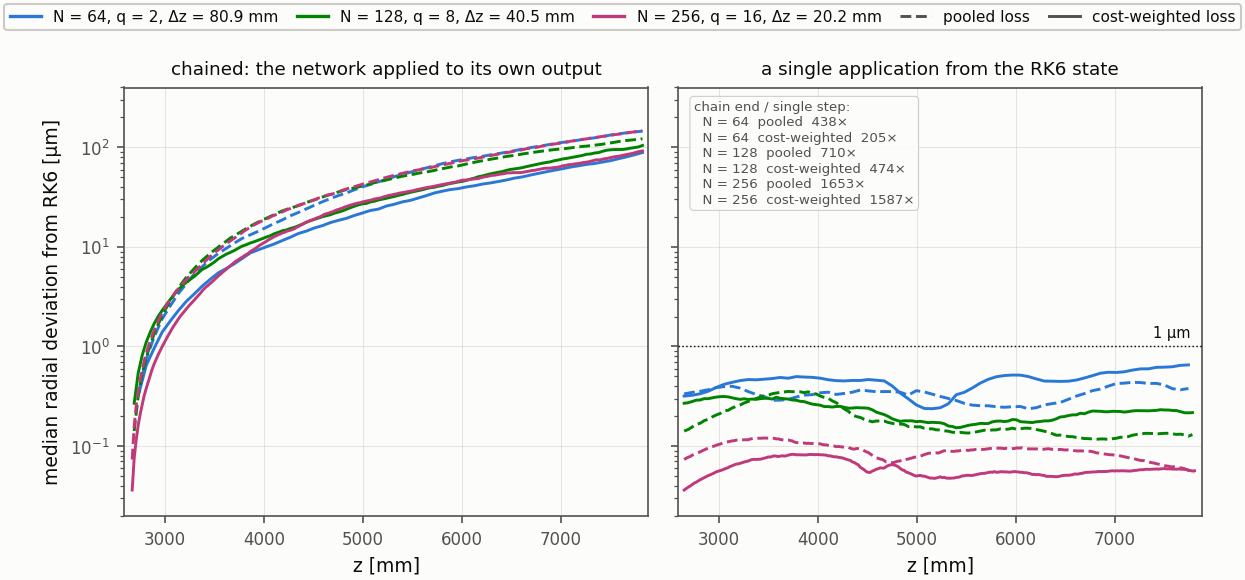
\includegraphics[width=0.95\linewidth]{fig_along_z.png}
  \caption{The error along the crossing: one step against the whole chain, for
  the six runs. Left: the median radial deviation from the reference at every
  plane of the chain, against $z$ from $z_0 = 2648.2\mm$ to $z_1 = 7826.0\mm$,
  micrometres on a logarithmic axis; the colour names the network and the
  pooled-loss run is dashed while the cost-weighted one is solid. Plane zero is
  the track's own starting state and is exactly zero, so the curves begin at the
  first output plane. Right: the same six networks applied \emph{once}, from the
  reference state on every start plane and compared with the reference one plane
  later, against the start plane's $z$ on the same scale. The two panels share
  their vertical range on purpose: a single application of any of these networks
  is well under one micrometre while the chain of $N$ of them ends near a
  hundred, and the ratio per run is printed in the right panel. No slopes appear
  in this figure. Source: \texttt{scripts/fig13\_along\_z.py}.}
  \label{fig:alongz}
\end{figure}

% ---------------------------------------------------------------------------
\subsection{Against the Geant4-true state}
\label{sec:results-truth}

Every number so far is a distance from a field-only reference, which answers how
well the network solves the problem it was given and not whether that problem is
the particle's real trajectory; this section puts all three reference points of
Section~\ref{sec:theory-references} on the same axis so that the distinction can
be read off.

\begin{table}[tbp]
  \centering
  \caption{The three reference points, per momentum band, for the three
  cost-weighted networks. \emph{nn--RK6} is the network against the field-only
  reference at $z_1$, \emph{nn--true} the same network's endpoint carried with
  the reference to the particle's own first SciFi plane and compared with its
  simulated state there, and \emph{RK6--true} the reference itself against that
  same state. Positions are the max metric $\max(|\Delta x|, |\Delta y|)$ in
  micrometres, slopes the max metric over the two slope components and
  dimensionless. \emph{RK6--true} does not depend on the network and is printed
  once per band. \emph{ratio} is RK6--true divided by nn--RK6 in position: how
  many times further the reference is from the truth than the network is from
  the reference. The $>50$ GeV band holds $30$ tracks. Source:
  \texttt{results/tab\_against\_true\_state.csv}.}
  \label{tab:truth}
  \footnotesize
  \setlength{\tabcolsep}{4pt}
  \begin{tabular}{llrrrrrrr}
    \toprule
    & & & \multicolumn{3}{c}{position, median [\!\um]}
        & \multicolumn{2}{c}{slope, median} & \\
    \cmidrule(lr){4-6}\cmidrule(lr){7-8}
    band [GeV] & network & $n$ & nn--RK6 & nn--true & RK6--true
      & nn--RK6 & nn--true & ratio \\
    \midrule
    $<3$ & $N = 64$, $q = 2$  & $164$ & $528.4$ & $9{,}338$ & $9{,}403$ & $4.73\times10^{-4}$ & $3.61\times10^{-3}$ & $17.8$ \\
         & $N = 128$, $q = 8$ & $164$ & $753.6$ & $9{,}785$ &           & $4.21\times10^{-4}$ & $3.57\times10^{-3}$ & $12.5$ \\
         & $N = 256$, $q = 16$& $164$ & $511.3$ & $9{,}365$ &           & $5.01\times10^{-4}$ & $3.48\times10^{-3}$ & $18.4$ \\
    \addlinespace
    $3$--$8$ & $N = 64$, $q = 2$  & $655$ & $159.4$ & $2{,}701$ & $2{,}699$ & $1.21\times10^{-4}$ & $8.71\times10^{-4}$ & $16.9$ \\
             & $N = 128$, $q = 8$ & $655$ & $198.1$ & $2{,}730$ &           & $1.26\times10^{-4}$ & $8.46\times10^{-4}$ & $13.6$ \\
             & $N = 256$, $q = 16$& $655$ & $157.0$ & $2{,}663$ &           & $1.35\times10^{-4}$ & $9.22\times10^{-4}$ & $17.2$ \\
    \addlinespace
    $8$--$20$ & $N = 64$, $q = 2$  & $433$ & $30.9$ & $736.4$ & $734.3$ & $2.49\times10^{-5}$ & $2.33\times10^{-4}$ & $23.8$ \\
              & $N = 128$, $q = 8$ & $433$ & $40.4$ & $758.2$ &         & $2.55\times10^{-5}$ & $2.22\times10^{-4}$ & $18.2$ \\
              & $N = 256$, $q = 16$& $433$ & $45.1$ & $745.7$ &         & $2.29\times10^{-5}$ & $2.19\times10^{-4}$ & $16.3$ \\
    \addlinespace
    $20$--$50$ & $N = 64$, $q = 2$  & $170$ & $15.7$ & $368.8$ & $369.2$ & $1.22\times10^{-5}$ & $1.11\times10^{-4}$ & $23.5$ \\
               & $N = 128$, $q = 8$ & $170$ & $19.8$ & $360.1$ &         & $1.19\times10^{-5}$ & $1.05\times10^{-4}$ & $18.6$ \\
               & $N = 256$, $q = 16$& $170$ & $18.2$ & $369.4$ &         & $1.10\times10^{-5}$ & $1.06\times10^{-4}$ & $20.3$ \\
    \addlinespace
    $>50$ & $N = 64$, $q = 2$  & $30$ & $20.7$ & $181.3$ & $182.8$ & $1.18\times10^{-5}$ & $4.67\times10^{-5}$ & $8.8$ \\
          & $N = 128$, $q = 8$ & $30$ & $29.3$ & $185.5$ &         & $1.17\times10^{-5}$ & $5.14\times10^{-5}$ & $6.2$ \\
          & $N = 256$, $q = 16$& $30$ & $44.4$ & $161.8$ &         & $2.76\times10^{-5}$ & $3.20\times10^{-5}$ & $4.1$ \\
    \addlinespace
    $10$--$50$ & $N = 64$, $q = 2$  & $487$ & $21.8$ & $555.7$ & $548.9$ & $1.80\times10^{-5}$ & $1.54\times10^{-4}$ & $25.2$ \\
    (window)   & $N = 128$, $q = 8$ & $487$ & $24.7$ & $555.0$ &         & $1.74\times10^{-5}$ & $1.52\times10^{-4}$ & $22.3$ \\
               & $N = 256$, $q = 16$& $487$ & $32.2$ & $552.7$ &         & $1.62\times10^{-5}$ & $1.50\times10^{-4}$ & $17.0$ \\
    \bottomrule
  \end{tabular}
\end{table}

Read it this way, one column pair at a time. The \emph{nn--true} and
\emph{RK6--true} columns are, to the eye, the same numbers. Over all test tracks
the network's median distance from the simulated truth is between $97.4$ and
$102.0$ per cent of the reference's own distance from it, across all six runs;
band by band, for the three cost-weighted networks, the largest departure from
unity anywhere in the table outside the thirty-track $>50$ GeV row is $4.1$ per
cent. The network and the reference are, at this resolution, the same object as
far as the real particle is concerned. That is not a coincidence and it is not a
measure of quality: it is the statement that the gap to the truth is the
material the particle crosses --- scattering and energy loss --- which neither
the reference nor the network models, and which is an order of magnitude larger
than the difference between them.

The \emph{ratio} column quantifies that. For the three cost-weighted networks
the reference is between $12.5$ and $25.2$ times further from the truth than the
network is from the reference, in every band from $<3$ to $20$--$50$ GeV and in
the loss window. Over all tracks the same ratio is $21.0$, $17.7$ and $20.1$.
For the pooled-loss networks it is more variable, from $2.7$ at $20$--$50$ GeV
to $31.7$ below $3$ GeV and $12.6$ to $15.4$ overall, because their distance
from the reference is both larger and more strongly momentum-dependent. The honest reading of the whole table is the one
Section~\ref{sec:theory-references} warned about: a network can be two to six
orders of magnitude above its own numerical ceiling
(Table~\ref{tab:grid}) and still be twenty times below the material term, and
both statements are true at once. The optimiser is the binding constraint on the
surrogate, and the surrogate is not yet the binding constraint on a track fit
that has to model the material anyway.

Two cautions belong here. First, the $>50$ GeV row holds $30$ test tracks; its
ratios are the smallest in the table, $8.8$, $6.2$ and $4.1$, and at $N = 256$,
$q = 16$ the network's distance from the truth is $88.5$ per cent of the
reference's, which is the only entry that departs from unity by more than a few
per cent. With thirty tracks that is one or two tracks' worth of median and
should be read as such. Second, this comparison cannot be used to score the
networks against one another. The network was never trained on the simulated
state, cannot reproduce it by construction, and the quantity that varies between
the six runs --- their distance from the reference --- is precisely the small
number being swamped. Figure~\ref{fig:threerefs} shows the arrangement.

\begin{figure}[tbp]
  \centering
  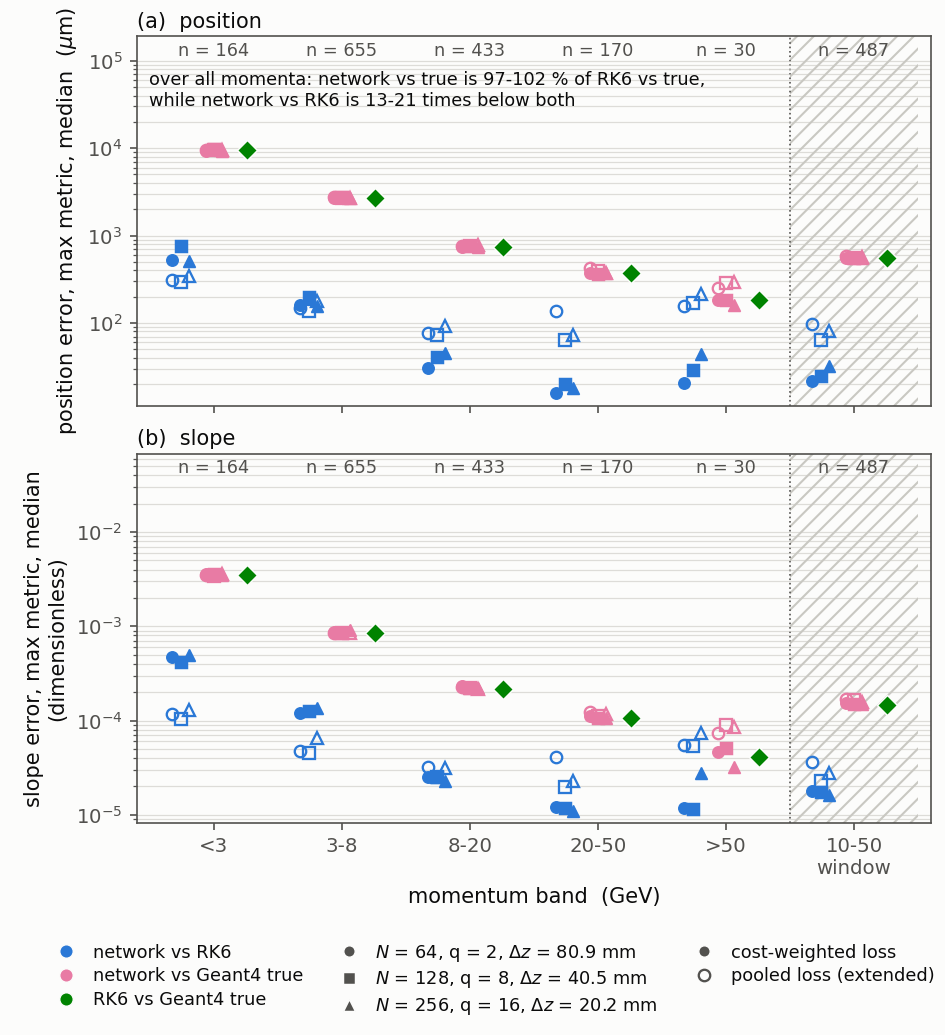
\includegraphics[width=0.85\linewidth]{fig_three_references.png}
  \caption{The three reference points for the same crossing, band by band. (a)
  The position error as the max metric $\max(|\Delta x|, |\Delta y|)$, median
  per band, in micrometres on a logarithmic axis, for the network against the
  field-only reference, the network against the particle's simulated state on
  its own first SciFi plane, and the reference against that same state. (b) The
  same for the slope, $\max(|\Delta t_x|, |\Delta t_y|)$, dimensionless, so the
  axis reads in scientific notation. Filled markers are the three cost-weighted
  networks and hollow markers the three pooled-loss networks extended to their
  own plateau, with the marker shape naming the network; the
  reference-against-truth point does not depend on the network and is drawn once
  per band. The five momentum bands are drawn as a partition and the
  $10$--$50$ GeV loss window, which overlaps two of them, is drawn apart on a
  hatched background; every band prints its $n$. The message is the vertical
  arrangement: network-against-truth and reference-against-truth sit on top of
  one another in every band, while for the three cost-weighted networks
  network-against-reference is more than an order of magnitude below both in
  every band from $<3$ to $20$--$50$ GeV and in the loss window. The
  thirty-track $>50$ GeV band is the exception: there the pooled-loss networks'
  hollow markers sit level with the reference-against-truth point, at ratios of
  $1.16$, $1.09$ and $0.85$, and the cost-weighted networks are a factor $4.1$
  to $8.8$ below rather than an order of magnitude. Source:
  \texttt{scripts/fig05\_three\_references.py}.}
  \label{fig:threerefs}
\end{figure}

% ---------------------------------------------------------------------------
\subsection{Cost}
\label{sec:results-cost}

The last thing to report is what all of this cost: what each network took to
train, and what a trained network costs to carry a track across the magnet.

\begin{table}[tbp]
  \centering
  \caption{What the six runs cost. \emph{restarts} is the number of optimiser
  restarts recorded, with the number of distinct restart indices beside it where
  the two differ; \emph{rounds} is the number of distinct rounds, with the
  number of recorded round rows beside it where the two differ. Every round is $25$ restarts and
  redraws $32{,}000$ collocation states, and every restart ran to the same
  iteration cap, a median of $200$ iterations, with no early stop anywhere.
  \emph{wall} is the total recorded training wall; \emph{per restart} its
  median over the de-duplicated history. \emph{carry} is the measured cost of
  taking one test track across the magnet with the trained network, the full
  chain of $N$ applications. Source: \texttt{results/tab\_compute.csv} and
  \texttt{results/paper\_numbers.json} (\texttt{compute}).}
  \label{tab:cost}
  \footnotesize
  \setlength{\tabcolsep}{4pt}
  \begin{tabular}{llrrrrrr}
    \toprule
    network & loss & params & restarts & rounds & per restart [s] &
    wall [h] & carry [\!$\mu$s/track] \\
    \midrule
    $N = 64$, $q = 2$   & pooled        & $18{,}956$ & $1{,}260$ & $50$ & $77.2$  & $31.2$  & $653$ \\
                        & cost-weighted & $18{,}956$ & $1{,}000$ & $40$ & $77.7$  & $21.6$  & $657$ \\
    \addlinespace
    $N = 128$, $q = 8$  & pooled        & $22{,}052$ & $1{,}599$ & $63$ & $117.9$ & $54.7$  & $1{,}353$ \\
                        & cost-weighted & $22{,}052$ & $1{,}000$ & $40$ & $118.3$ & $32.8$  & $1{,}322$ \\
    \addlinespace
    $N = 256$, $q = 16$ & pooled        & $26{,}180$ & $1{,}050$ & $42$ & $219.8$ & $63.2$  & $2{,}964$ \\
                        & cost-weighted & $26{,}180$ & $1{,}807$ ($1{,}500$) & $60$ ($74$) & $184.1$ & $100.4$ & $3{,}655$ \\
    \bottomrule
  \end{tabular}
\end{table}

Read it this way. The two losses cost the same to train. At every step length
the median wall per restart differs between the two by less than half a per
cent --- $77.2$ against $77.7$ seconds, $117.9$ against $118.3$, and $219.8$
against $184.1$, the last being the one affected by the duplicate job discussed
below. The reweighting changes the weights inside the loss and nothing else, so
this is what one would expect, and it is worth recording because a cheaper
objective that cost more to optimise would be a different result. The total
walls differ only because the runs were given different numbers of restarts.
The per-restart cost roughly follows the arithmetic of a step: $N$ applications
of a network emitting $4(q+1)$ numbers, with $q$ field lookups each, gives
$N \times q$ field evaluations per crossing, which is $128$, $1024$ and $4096$
at the three working points, and the measured walls are in the ratio
$1 : 1.53 : 2.85$ rather than $1 : 8 : 32$, because the batch is large and much
of the per-restart cost is not the field.

The duplicate-job note has to be stated plainly because it affects one row.
The $N = 256$, $q = 16$ cost-weighted run was trained by two farm jobs at once
from restart $1{,}198$ onwards. Its history file therefore holds $302$ repeated
restart numbers and its round file $13$ repeated round numbers: $1{,}807$
history rows for $1{,}500$ distinct restarts, and $74$ round rows for $60$
distinct rounds. Every reader of those files in this paper de-duplicates them by
keeping the last row written per number, which is the rule the analysis folder
already used, and the restart and round counts quoted everywhere in this paper
are the de-duplicated ones. The wall is the one quantity where the two
bookkeepings genuinely disagree: the run's own record says $100.4$ hours, which
counts the duplicate job's work, while the de-duplicated history sums to
$81.1$ hours. The table quotes the recorded $100.4$ hours, since that is what
the farm actually spent, and the reader should know that about $19$ hours of it
was work done twice. No other run in the set has a duplicated row.

The carry cost is a measurement of this implementation and not a deployment
figure, and I say so rather than letting it be read as one. It is $653$ to
$657\,\mu$s per track at $N = 64$, $1{,}322$ to $1{,}353$ at $N = 128$ and
$2{,}964$ to $3{,}655$ at $N = 256$, measured in the same framework the
networks were trained in, on one thread, with no fusion, no reduced precision
and no attempt at optimisation. For scale, the sixth-order reference integrating
the same crossing at $0.1\mm$ steps costs about $0.12$ seconds per track when
amortised over a large batch, so the $N = 64$ network is already about $180$
times faster than the reference it is being scored against --- but the reference
is a double-precision research integrator taking fifty thousand steps, not the
production extrapolator, and the comparison that matters for the trigger is
against the latter and has not been made here. What the table does establish is
the scaling: the carry cost doubles with each halving of the step, as it must,
so the shortest-step network costs four and a half to five and a half times the
longest-step one and
delivers, by Section~\ref{sec:results-shortersteps}, no better a crossing. That
is a second and independent reason not to take the step length below
$\Delta z = 80.9\mm$ on this evidence.

% ===========================================================================
\section{The low-momentum window (reserved)}
\label{sec:lowmom}

\begin{quote}
\fbox{\parbox{0.92\linewidth}{%
\textbf{Reserved.} This section is held for the study in which the momentum
window of Eq.~\eqref{eq:window} is moved down onto the $3$--$8$\,GeV band.
Those runs are \textbf{in training at the time of writing}, so no number from
them is reported here. When they land, this section will report them in exactly
the form Sections~\ref{sec:results-headline} to \ref{sec:results-5gev} use for
the $10$--$50$\,GeV runs: the headline comparison of the same chained networks
under the moved window against the same pooled-loss counterparts, as
Table~\ref{tab:headline}; the radial endpoint median and $95$th percentile in
the paper's five momentum bands with the moved window as the extra row, as
Table~\ref{tab:headlinebands}; and the per-component breakdown, as
Tables~\ref{tab:comppos} and \ref{tab:compslope}, with the region around
$5$\,GeV treated as in Section~\ref{sec:results-5gev}. The same three reference
points of Section~\ref{sec:theory-references}, the same plateau rule and the
same test tracks apply, so the effect of moving the window can be read off
directly against Section~\ref{sec:results}.}}
\end{quote}


\section{Discussion}
\label{sec:discussion}

Section~\ref{sec:results} reported the experiment; this section reads it
against the two questions of Section~\ref{sec:intro-questions}. I take the
improvement first (Section~\ref{sec:discussion-did}), then the price
(Section~\ref{sec:discussion-didnot}), then everything that limits how far
either half can be pushed (Section~\ref{sec:discussion-caveats}). No new
measurement appears here; every number has already been given a table and a
source above.

\subsection{What the reweighting did}
\label{sec:discussion-did}

The experiment had a pre-registered outcome and it is the full one.
Section~\ref{sec:theory-metrics} fixed two conditions in advance, and
Section~\ref{sec:results-headline} tested them on the $N = 64$, $q = 2$,
$\Delta z = 80.9\mm$ pair. The first was that the test radial endpoint error
clear a $\pm 13$ per cent run-to-run band downward: it falls from $145.7$ to
$88.8\um$, by $39.1$ per cent, which clears that band and also clears the
$\pm 17.5$ per cent round-to-round spread the counterpart turned out to have.
The second was that the median per-step slope error fall below
$1.6\times10^{-6}$: the cost-weighted network reaches $7.34\times10^{-7}$ in
$t_x$, a factor $2.18$ below the threshold. Both hold.

The second condition is the weaker of the two and I say so rather than
counting it twice. The extended pooled-loss counterpart has itself fallen to
$1.30\times10^{-6}$ since the threshold was written, which is also below
$1.6\times10^{-6}$, so that condition no longer separates the two losses. What
separates them is the first condition and the size of the margin on it.

\paragraph{The gain is concentrated where the weight was put.} Inside the
$10$--$50$ GeV loss window the $N = 64$ median endpoint error falls from
$108.1$ to $24.8\um$, a factor $4.37$. That is the one feature common to all
three step lengths: the same window falls by a factor $2.58$ at $N = 128$ and
$2.59$ at $N = 256$, so the in-window gain is a factor between $2.6$ and $4.4$
everywhere it was measured. It is visible one derivative down as well. In the
window the median per-step $x$-slope error falls from $9.49\times10^{-7}$ to
$2.25\times10^{-7}$, a factor $4.21$, against factors of $3.08$ and $3.21$ at
the two shorter steps. The endpoint gain and the per-step gain are the same
size, which is what Section~\ref{sec:results-anatomy} says they must be:
modelling the endpoint error as accumulated per-step error carried by the
lever arm reproduces the measured radial endpoint error to between $97.7$ and
$99.4$ per cent in all six runs, so there is nothing between the step and the
endpoint for the two numbers to disagree about.

The pre-flight of Section~\ref{sec:results-weight} says why this happened, and
it was measured before any reweighted network existed. The share of the loss
carried by the loss window rises from $1.23$ to $47.0$ per cent, the share
carried by the $3$--$8$ GeV band falls from $89.8$ to $38.3$, the share carried
by the first quarter of the crossing --- where an error has the longest lever
arm --- rises from $0.65$ to $23.3$ per cent, and within the window the rank
correlation between a state's share of the loss and what that state's error
actually costs at $z_1$ rises from $+0.532$ to $+0.896$. The objective was
asked to look somewhere else and it did, and the endpoint error followed it
there.

\paragraph{The whole of the gain is in $x$.} Over all test tracks the median
$|\Delta x|$ at the first SciFi plane falls from $110.7$ to $37.5\um$, a factor
$2.95$, while the median $|\Delta y|$ moves from $52.3$ to $55.2\um$, which is
$5.6$ per cent worse. The magnet's field is close to vertical and therefore
bends the track horizontally, so $x$ is where the correction the surrogate has
to reproduce lives, and $x$ is what the reweighting improved. Inside the window
both components do fall --- $86.9$ to $11.6\um$ in $x$ and $39.6$ to
$13.9\um$ in $y$ --- but their ordering swaps: under the pooled loss the $x$
error is $2.2$ times the $y$ error there, and under the cost-weighted loss the
$y$ error is the larger by a factor $1.20$. What limits the reweighted network
inside its own window is now the non-bending plane.

\paragraph{The in-window offset falls in every pair.} The signed median is the
sharper statement, because a signed median close to the median magnitude is a
common offset in one direction rather than scatter. In the window the
pooled-loss $N = 64$ network sits at $-54.4\um$ in $x$ against a median
magnitude of $86.9\um$, and the cost-weighted one at $-6.3\um$ against
$11.6\um$: the absolute offset falls by a factor $8.7$. The same happens at the
other two step lengths, from $+17.9$ to $+0.15\um$ at $N = 128$ and from
$+30.3$ to $-2.7\um$ at $N = 256$. So the absolute in-window offset falls in
all three pairs. As a fraction of the error's own size it falls in two of the
three, from $0.33$ to $0.011$ at $N = 128$ and from $0.44$ to $0.22$ at
$N = 256$, while at $N = 64$ it is $0.63$ before and $0.54$ after, which is
barely a change. And the sign of the pooled-loss offset is not common to the
three: it is negative at $N = 64$ and positive at $N = 128$ and $N = 256$. The
defensible claim is therefore the one Section~\ref{sec:results-components}
makes and no more: the reweighting reduces the in-window offset in absolute
terms everywhere and relative to the error in two of three pairs. It is not
that it removes a systematic under-bend, because there is no single under-bend
across the three to remove.

\paragraph{None of this cost the label-free property.} Both factors of
Eq.~\eqref{eq:lossF} are functions of the network's own inputs and of the
measured field map: the lever arm is geometry, and the track factor needs
$|q/p|$, which is the fifth component of the input, and the field integral
$\bar{I}$. No reference trajectory, from an integrator or from a simulation,
enters the weight, so the property that makes the construction worth having is
intact. The weight was also checked not to move the minimum before any network
was trained: collocation states solved exactly by a root-finder give between
$6\times10^{-30}$ and $2\times10^{-29}$ of the straight line's loss under every
weighting mode, which is machine zero. The reweighting changes the shape of the
surface around the minimum and not where the minimum is.

\subsection{What it did not do}
\label{sec:discussion-didnot}

\paragraph{It is worse below the crossover.} The crossover sits between the
$3$--$8$ and the $8$--$20$ GeV bands, and below it the cost-weighted network is
worse in five of the six comparisons. The exception is the $3$--$8$ GeV band at
$N = 256$, where the median falls from $200.4$ to $177.7\um$, a reduction of
$11.3$ per cent. At $N = 64$ the median below
$3$ GeV rises from $353.7$ to $615.1\um$, a factor $1.74$; the $95$th
percentile over all tracks rises from $898$ to $1399\um$, a factor $1.56$; and
the fraction of tracks ending more than a millimetre from the reference rises
from $4.41$ to $7.16$ per cent, which is $64$ tracks becoming $104$. At
$N = 128$ the degradation below $3$ GeV is the largest anywhere in the paper, a
factor $2.70$ in the median and a $95$th percentile that more than doubles to
$3.67\mm$. This is a trade and it was the trade the objective was designed to
make, since the window was written into the loss deliberately; but a
surrogate that has to serve every track in the event does not get to ignore
the half of the population that sits below $8$ GeV, and the price is therefore
real rather than presentational.

\paragraph{The vertical plane did not move.} Over all tracks the median
$|\Delta y|$ is $52.3\um$ under the pooled loss and $55.2\um$ under the
cost-weighted one at $N = 64$; at $N = 128$ it goes from $59.2$ to $61.2\um$
and at $N = 256$ from $69.7$ to $61.3\um$. Across the three pairs the $x$ error
improves by between $1.6$ and $7.5$ times and the $y$ error by between $0.95$
and $2.9$. The effect is already present in a single step: the per-step
$|\Delta t_y|$ over all tracks is worse under the cost-weighted loss in all
three pairs, $9.74$ against $7.16$, $4.98$ against $3.15$ and $2.38$ against
$1.83$, in units of $10^{-7}$, and in the $3$--$8$ GeV band the cost-weighted
$t_y$ error is $2.2$, $2.2$ and $1.8$ times the pooled one. Near $5$ GeV the
vertical distribution has both shifted and widened: in the $4$--$6$ GeV band
the signed median in $y$ goes from $-9.2$ to $+28.1\um$ and the $68$ per cent
half-width from $96.6$ to $223.3\um$, and in $t_y$ the half-width goes from
$3.97\times10^{-5}$ to $1.61\times10^{-4}$. Equation~\eqref{eq:lossF} weights
the two position components equally, in millimetres, because the endpoint
measure is radial, so nothing in the objective pushed on $y$; what the
reweighting did was remove the term that had been holding $x$ down, and $y$ was
left where it was or slightly worse.

\paragraph{What is left is more coherent, not less.} The per-step errors of a
chain can add or cancel, and Section~\ref{sec:theory-metrics} measures which by
dividing the magnitude of the sum of the per-step slope errors by the sum of
their magnitudes. Independent steps would give $1/\sqrt{N}$, that is $0.125$,
$0.0884$ and $0.0625$ at the three step counts. The measured values run from
$0.31$ to $0.53$, so every chain in this paper is between $2.9$ and $7.6$ times
more aligned than chance --- and the cost-weighted networks are the more
aligned of each pair in all six of the matched comparisons, $0.491$ and $0.518$
against $0.357$ and $0.397$ at $N = 64$, $0.527$ and $0.459$ against $0.312$
and $0.432$ at $N = 128$, and $0.454$ and $0.474$ against $0.411$ and $0.453$
at $N = 256$. Smaller per-step errors that all point the same way accumulate as
efficiently as larger random ones, so part of the per-step gain was handed
back at the endpoint. The same shift shows in the decomposition: a model built
from the $x$ slope alone recovers $63$ to $73$ per cent of the endpoint error
under the pooled loss and only $36$ to $45$ per cent under the cost-weighted
one. The error that remains is a coherent drift and it is no longer confined to
one plane.

\paragraph{The heavy tail is geometric, not a matter of momentum.} The tracks
that end more than a millimetre from the reference are not scattered through
the population. In the $3$--$8$ GeV band under the cost-weighted loss their
median starting $|x|$ on the last Upstream Tracker plane is $217.1\mm$ against
$107.8\mm$ for the rest of the band, a ratio of $2.01$; under the pooled loss
the same ratio is $1.46$, and in the narrower $4$--$6$ GeV band the two ratios
are $1.66$ and $1.39$. The tail is made of soft tracks that start far from the
beam line, and the reweighting made it more so. A momentum window cannot reach
this, because the variable that distinguishes the tail is not momentum. That is
a concrete statement about what the next weight would have to contain, and it
is in Section~\ref{sec:outlook}.

\paragraph{Shortening the step did not help.} The design has a free parameter
the first study did not have, and the obvious expectation is that a shorter
step is an easier problem. Each step does get easier: under the pooled loss the
per-step radial error goes $0.333 \to 0.172 \to 0.089\um$ as $\Delta z$ is
halved twice, ratios of $1.93$ and $1.93$, and under the cost-weighted loss the
per-step $x$-slope error goes $7.34 \to 3.77 \to 1.87$ in units of $10^{-7}$,
ratios of $1.95$ and $2.02$. The crossing does not follow. The pooled-loss
endpoint goes $145.7 \to 122.2 \to 147.7\um$ and the cost-weighted one
$88.8 \to 104.6 \to 92.2\um$: neither is monotone and neither moves by more
than a factor $1.21$ across a factor four in step length. Inside the loss
window the cost-weighted sequence is $24.8 \to 27.3 \to 34.6\um$, which gets
steadily worse, so the network with the smallest per-step error has the largest
in-window endpoint error of the three. The coherences above are the reason: a
perfectly incoherent chain would improve as $\sqrt{\Delta z}$ and a perfectly
coherent one not at all, and these chains sit much nearer the coherent limit.
The chain's endpoint error is $438$ and $205$ times its own single-step error
at $N = 64$, $710$ and $474$ at $N = 128$ and $1653$ and $1587$ at $N = 256$,
against the $8$, $11$ and $16$ that $\sqrt{N}$ independent steps would give.
Since the measured carry cost doubles with each halving of the step, the
shortest-step network costs four and a half to five and a half times the
longest-step one and delivers no better a crossing. On this evidence there is
no reason to go below $\Delta z = 80.9\mm$.

\subsection{Caveats, stated plainly}
\label{sec:discussion-caveats}

\begin{itemize}
  \item \textbf{Two of the three pooled-loss runs had not finished training.}
  Applying the plateau rule of Section~\ref{sec:theory-metrics} to the six
  runs' own round logs, all three cost-weighted runs are flat at their last
  round and only one of the three pooled-loss runs is. The $N = 128$, $q = 8$
  pooled run was still improving at $7.24$ per cent per ten rounds when it
  stopped at round $63$, and the $N = 256$, $q = 16$ pooled run at $10.94$ per
  cent per ten rounds at round $42$, after both had already been extended well
  past the stopped snapshot. Their rows are lower bounds on how good those
  networks would eventually be, so the margins at those two step lengths are
  upper bounds on the effect of the loss. \textbf{The conclusions of this paper
  therefore rest on the $N = 64$, $q = 2$ pair}, which is the pre-registered one
  and the only pair in which both sides are flat; the other two pairs are
  reported in full and are read as supporting evidence rather than as
  independent evidence.
  \item \textbf{One seed.} Every run in this paper uses seed $0$
  (Table~\ref{tab:fixed}). There is no seed ensemble anywhere, so the only
  measure of run-to-run variation available is the round-to-round spread of the
  validation headline, which is $17.5$, $11.7$, $12.4$, $10.8$, $9.8$ and
  $25.9$ per cent over the six runs. That is why the pre-registered criterion
  was written as a band to be cleared rather than as an inequality between two
  medians, and it is why no difference of order ten per cent anywhere in this
  paper should be read as a difference.
  \item \textbf{The stiffest band is thirty tracks.} The $>50$ GeV band holds
  $30$ test tracks. Its medians move by factors of $5$ to $8$ between the two
  losses, among the largest in Table~\ref{tab:headlinebands} --- whose largest
  factor is the $9.01$ of the $20$--$50$ GeV band at $N = 64$ --- and a
  band of that size cannot support a quantitative claim. It is read here only as
  agreeing in direction with the $20$--$50$ GeV band beside it.
  \item \textbf{The three ablations were never trained.} The lever-arm-off,
  track-factor-off and window-off columns of Table~\ref{tab:preflight} are
  pre-flight diagnostics: one factor of Eq.~\eqref{eq:lossF} is replaced by its
  own average on a network that was trained under a different objective
  entirely. They say how each factor redistributes a fixed set of residuals.
  They do not say what a network trained under any of them would do, and no such
  network exists.
  \item \textbf{The output parameterisation was chosen for the earlier fixed-step study
  and inherited here.} Every
  network in this paper writes its outputs as the straight-line extrapolation of
  the input plus a per-track-scaled correction (Eq.~\eqref{eq:netparam}), so it
  learns the correction to the straight line rather than the stage states that
  the network of Raissi, Perdikaris and Karniadakis emits. The form was
  introduced for a network serving step lengths from $70\mm$ to $8.6$ m, chosen
  explicitly for the earlier fixed-step study, and inherited by this paper's
  single-network chain without re-examination. Its effect here
  is unmeasured: no network in this paper was trained to emit the stage states
  directly, so nothing in Section~\ref{sec:results} says whether any of its
  numbers depends on the choice, in either direction.
  \item \textbf{The pre-flight was measured on the extended network, not on the
  checkpoint the original gate used.} The stored record of this measurement was
  taken on the stopped checkpoint of 18 September 2026, and the numbers in
  Table~\ref{tab:preflight} are the same measurement on the extended network.
  Re-running the pre-flight on that checkpoint reproduces the stored record
  exactly, to zero deviation in every row, so the method and the replayed random
  draw are the ones the original gate used; but the two sets of numbers differ
  by $0.2$ to $8.5$ per cent, because the weights are identical and the
  residuals they weigh are not. The largest of those differences is the
  cost-weighted loss's share of the $10$--$50$ GeV window, and the value in this
  paper is the smaller one.
  \item \textbf{The reference is field-only.} Every network number in this paper
  is a distance from a sixth-order integration of the equation of motion in the
  measured field, and Section~\ref{sec:scheme-fieldonly} measures what that
  equation leaves out: a median of $1736\um$ between the field-only reference
  and the simulated particle over the whole set, $532\um$ in the loss window and
  $153\um$ above $50$ GeV. Part of that gap is a defect in my own pipeline, a
  start momentum that is the particle's production momentum and implies an
  over-bend worth $+17.6$, $+17.3$ and $+12.2$ MeV in the three bands below
  $20$ GeV; part is energy loss along the crossing, which the equation does not
  model; part is multiple scattering, which is stochastic and irreducible; and
  the momentum-growing residual above $20$ GeV is unexplained. None of this
  moves a single network-against-reference number, because the network and the
  reference share the same equation and the same $q/p$. What it does mean is
  that the levels in Section~\ref{sec:results-truth} are the levels that decide
  whether any of this yet matters physically.
  \item \textbf{The carry cost is a framework number, not a deployment number.}
  The $653$ to $657\,\mu$s per track at $N = 64$, and the figures at the two
  shorter steps, were measured in the same framework the networks were trained
  in, on one thread, in double precision, with no fusion and no attempt at
  optimisation. The comparison that matters for the trigger is against the
  production extrapolator in the deployment precision on the deployment
  hardware, and it has not been made here. What the measurement does establish
  is the scaling with $N$, which is the part the design choice turns on.
  \item \textbf{Two of the sixteen exact ceilings are not fresh solves.} The
  exact collocation scheme was solved for this paper at $N = 2$ and $N = 256$
  and stored per component; the $N = 64$ and $N = 128$ cells of
  Table~\ref{tab:ceiling} are read from the earlier chained comparator table,
  which stores the radial median alone. That is why the max-metric block of that
  table is empty in those two rows. It does not affect the reading, because the
  point those cells carry is that the ceiling is orders of magnitude below the
  networks and not what its third digit is.
\end{itemize}

% ===========================================================================
\section{Outlook}
\label{sec:outlook}

Seven things follow from the result and from how it was built, in the order in
which they are worth doing.

\paragraph{1. The rework: emit the stage states directly.} Every network in this
paper learns the correction to the straight line, a form inherited from a
network that served steps of very different lengths and never re-examined here
(Section~\ref{sec:theory-chaining}). The direct test is to retrain the same
chain with the network emitting the stage states and the endpoint directly, as
in the source construction, with the same two losses and everything else
identical, starting with $N = 64$, $q = 2$. If the chain reaches the same
endpoint error, the form was not load-bearing here and the design is closer to
its source than it looked; if it does not, the correction to the straight line
is part of why the chain works, and that belongs in the description of the
method rather than in its implementation.

\paragraph{2. The window moved down onto $3$--$8$ GeV.} The clearest test of
the claim made here is to move the loss window and see whether the trade moves
with it. Those runs are built, they have passed the same gates as the runs
reported above, and they are in training as this is written;
Section~\ref{sec:lowmom} is reserved for them and states what it will contain.
The expected outcome is a trade in the opposite direction: the $3$--$8$ GeV
band should improve by something like the factor the $10$--$50$ GeV window
improved by here, and the $10$--$50$ GeV band and the tail should pay for it.
If that is what happens, the weight is behaving as a knob rather than as an
improvement, which is the more useful thing to know; if the soft band does not
improve, then the soft tracks are hard for a reason the weight cannot reach,
and the tail measurement above says where to look next.

\paragraph{3. Train the three ablations.} The three diagnostic columns of
Table~\ref{tab:preflight} say how the lever arm, the per-track factor and the
momentum window each redistribute a fixed set of residuals, and they say it
cleanly: the lever arm is the whole of the $z$ redistribution and none of the
momentum redistribution, the per-track factor does the bulk of the momentum
work and the window finishes it. What they cannot say is which factor produced
the endpoint gain, because no network was trained under any of them. Three runs
at $N = 64$, $q = 2$, each with one factor switched off and everything else
identical, would settle that in the same way the pre-registered pair settled the
full weight, and at the same cost as the pair.

\paragraph{4. Supervise the step Jacobian.} The binding constraint is not the
size of a single step's error but the fact that successive steps make the same
error. The chains here are between $2.9$ and $7.6$ times more aligned than
independent steps would be, and the cost-weighted chains are the more aligned
of each pair, so the accumulation absorbed part of the per-step gain. Nothing in
either objective refers to more than one step at a time, which is why the
alignment is free to be whatever the map happens to produce. A term that reads
the derivative of one step's output with respect to its input --- the step
Jacobian --- and asks it to match the Jacobian the collocation equations imply
would constrain how an error made at step $k$ is carried into step $k+1$, and
it would still be label-free, since the collocation equations and the field map
are all it needs. This is the item with the most room in it: the decomposition
of Section~\ref{sec:results-anatomy} says the endpoint error is accumulated
per-step error and nothing else, so anything that breaks the alignment goes
straight to the endpoint.

\paragraph{5. Weight on the starting geometry, not only on the momentum.} The
tail is made of soft tracks that start far from the beam line: a median
starting $|x|$ of $217.1\mm$ against $107.8\mm$ for the rest of the same band.
Both weights in this paper are blind to that, because both are built from
momentum and from position in $z$. A factor in $a_n$ that rises with the
track's starting $|x|$, or with the straight-line path's distance from the axis,
would be as cheap and as label-free as the two factors already there, and it
would act on the one population that neither loss currently reaches. The tail
is also the quantity a real-time system schedules against, so it is worth more
than its share of the median suggests.

\paragraph{6. Settle the reference.} Section~\ref{sec:scheme-fieldonly} leaves
two loose ends and both are cheap to close. The first is the start momentum:
the state harvesting joins the momentum from the particle table, which is the
particle's production momentum, and the truth dump never wrote the hit's own
local momentum, which the simulation records. Re-dumping the truth with the
local momentum would separate the energy the particle lost before the start
plane from the energy it loses in the crossing, which is the difference between
a pipeline defect and a piece of physics the equation is missing; at present the
two are summed into one $+17$ MeV. The second is the material itself. The
measured scattering width is a stable $2.1$ to $2.3$ times the air-only
prediction above $8$ GeV and implies $6.8$ to $8.1$ per cent of a radiation
length against the $1.70$ per cent air provides, which is a measurement of the
simulation's material budget and not a confirmation of it, because I have not
looked that budget up independently. Doing so would say whether the remaining
factor is material that is known to be there. Neither item changes a network
number, and both change what the numbers mean.

\paragraph{7. The cost comparison that has not been made.} The argument for a
surrogate is that its arithmetic is fixed and known before the track arrives,
and this paper supports that argument with an operation count and a framework
measurement, not with a deployment measurement. The $N = 64$ network carries a
track across the magnet in $653$ to $657\,\mu$s in double precision on one
thread with no optimisation, about $180$ times faster than the double-precision
research integrator it is scored against; but that integrator takes fifty
thousand steps and is not the production extrapolator. The comparison that
decides anything is against the production routine, in reduced precision, on
the hardware the trigger runs on~\citep{aaij2020}, and until it is made the cost
argument remains a promise.

% ===========================================================================
\section{Conclusion}
\label{sec:conclusion}

One small neural network, trained to take a single fixed step in $z$ and then
applied to its own output as many times as it takes to cross the LHCb magnet,
solves a problem the first study of this programme left
open~\citep{scriven2026lhcb1}. There, a single network asked to cross the
magnet in one $5178\mm$ step, inside a network that also served every other
kind of step, sat a factor $22$ above the numerical scheme it was being trained
to solve, and that one leg dominated everything chained to it. Cutting the same
crossing into $64$ steps of $80.9\mm$ and training one network to take a step
of that length, wherever in the crossing it starts, removes the discretisation
from the problem entirely: the exact collocation scheme chained the same $64$
times sits $0.147\um$ from the reference, so every trained network in this paper
is limited by its own optimisation and by the accumulation along the chain, and
not at all by the scheme. That is the fact everything else rests on, and it was
measured rather than assumed.

The experiment this paper reports is a change of objective on that design.
Under the loss the construction comes with, the network reaches a median
endpoint error of $145.7\um$ over $1452$ held-out tracks, and the pre-flight
shows where that loss spends itself: $89.8$ per cent on tracks of $3$--$8$ GeV,
$1.23$ per cent on the $10$--$50$ GeV momentum region of interest, and $0.65$
per cent on the quarter of the crossing where an error has the furthest to
travel. Replacing it with a loss that measures every residual by the
displacement it would cause at the far side of the magnet, as a fraction of
that track's own total bend and with the region of interest weighted up, moves
the endpoint error to $88.8\um$ and the in-window error from $108.1$ to
$24.8\um$, a factor $4.37$. The median per-step slope error in $t_x$ falls from
$1.30\times10^{-6}$ to $7.34\times10^{-7}$. Both pre-registered conditions are
met, although the second is weak, because the pooled-loss counterpart has since
fallen below that threshold as well. The new weight is built from the network's
own inputs and the measured field map alone, so the objective is still
label-free in the precise sense of this paper: no reference trajectory enters
it anywhere. Measured against the particle's simulated state rather than
against the field-only reference, the network and the reference are
indistinguishable --- the network's median distance from the simulated truth is
between $97.4$ and $102.0$ per cent of the reference's own distance from it
across all six runs --- because both omit the material the particle crosses,
and that omission is, for the three cost-weighted networks, between $12.5$ and
$25.2$ times larger than the difference between them in every band from $<3$ to
$20$--$50$ GeV and in the loss window. In the thirty-track $>50$ GeV band the
pooled networks instead approach the reference-to-truth gap, the ratio falling
to $0.85$.

The negatives are as specific as the gain. The improvement is a trade, not a
free lunch: below the crossover between $3$--$8$ and $8$--$20$ GeV the
reweighted network is worse in five of six comparisons, the median below $3$ GeV
rises from $353.7$ to $615.1\um$, the $95$th percentile over all tracks rises
from $898$ to $1399\um$, and the fraction of tracks ending more than a
millimetre away rises from $4.41$ to $7.16$ per cent. The whole of the gain is
in the bending plane; the vertical plane does not move, and inside the window it
becomes the larger of the two errors. What is left is more coherent than what it
replaced, in all six matched comparisons, which is why a factor of four in the
per-step slope error did not become a larger factor at the endpoint. Shortening
the step from $80.9$ to $20.2\mm$ halves each step's error and does not improve
the crossing at all, while costing four and a half to five and a half times as
much to carry a track. And the heavy tail is made of soft tracks that start far
from the beam line, which no momentum window can reach.

Two of the three pooled-loss runs had not finished training when they were
stopped, so the conclusions rest on the one pair in which both sides had; there
is one seed; the stiffest band holds thirty tracks; the network's outputs are
written as a correction to the straight line, a form chosen for the earlier
fixed-step study and inherited here, whose effect in this design has not been
measured; and the deployment cost
comparison has not been made. What the paper establishes is narrower than the
headline and more useful: on this design the endpoint error is accumulated
per-step error carried by the lever arm and nothing else, to between $97.7$ and
$99.4$ per cent, the objective decides where that error sits in momentum and in
$z$, and the accumulation --- not the size of a single step --- is what now
limits the crossing.

% ===========================================================================
\section*{Data availability}
\addcontentsline{toc}{section}{Data availability}

The code, the committed result tables and the figures are in the repository
\texttt{LHCb\_Extrapolation\_Project} at
\url{https://github.com/GeorgeWilliam1999/LHCb-Extrapolation}. Everything the
experiments of this paper produced --- the track set builder, the six training
runs, the comparators, the analysis folders and the reference-against-truth
study, that is the whole
\texttt{single\_network\_chain\_discrete\_approach/} tree --- is committed as
\texttt{b84693f7} on \texttt{main}.

Two things are not in that commit. The paper folder
\texttt{Self\_chained\_paper/}, which holds this source, its scripts, its
committed result files and its figures, is untracked at the time of writing and
will be committed by George. The figure supplement
\texttt{single\_network\_chain\_discrete\_approach/data\_supplement/} was
committed afterwards, as \texttt{aac1692f}.

Every figure in this paper is regenerated by a script in
\texttt{Self\_chained\_paper/scripts/} from committed result files only; no
figure is copied in from an experiment folder. The pipeline is two commands
from inside \texttt{Self\_chained\_paper/}: first
%
\begin{quote}
\texttt{PYTHONNOUSERSITE=1 /data/bfys/gscriven/conda/envs/TE/bin/python scripts/numbers.py}
\end{quote}
%
which reads the experiment folders read-only and writes
\texttt{results/paper\_numbers.json}, the \texttt{results/tab\_*.csv} tables and
the \texttt{results/cache/} arrays; then each of
\texttt{scripts/fig01\_crossing.py} to
\texttt{scripts/fig17\_loss\_weights\_schematic.py} in turn,
each of which writes one PNG into \texttt{figures/} and one companion
\texttt{results/fig*.csv} carrying the numbers it drew. Model weights and the
track set itself are not committed; they regenerate from the recorded seed, the
committed metadata and the scripts. Appendix~\ref{sec:provenance} gives the
commits, the data set, the cluster identifiers and the maps from every figure
and every table to the file it was computed from.

% ===========================================================================
\appendix
\section{Provenance}
\label{sec:provenance}

This appendix is the audit trail. It is the only part of the paper in which
experiment folder names, block letters and cluster identifiers appear; the body
names networks by their step count $N$, their stage count $q$ and their step
length $\Delta z$, and nothing else.

\subsection*{Repository and commits}

Repository \texttt{LHCb\_Extrapolation\_Project},
\url{https://github.com/GeorgeWilliam1999/LHCb-Extrapolation}, branch
\texttt{main}. Local checkout
\texttt{/data/bfys/gscriven/LHCb\_Extrapolation\_Project}.

\begin{itemize}
  \item \texttt{b84693f7} (22 September 2026), ``Single-network chain across the
  magnet: Blocks E, F, G; reference-vs-truth study; write-up plans''. This is
  the commit every number in this paper traces to. It carries the whole
  \texttt{single\_network\_chain\_discrete\_approach/} tree: the track set
  builder and its gates (\texttt{Block\_E\_single\_network\_chain/}\allowbreak\texttt{E0\_Track\_dataset/}),
  the sixteen pooled-loss runs and their extensions
  (\texttt{E1\_Network\_grid/}), the exact-collocation comparators
  (\texttt{E2\_Comparators/}), the pooled-loss analysis
  (\texttt{E3\_Analysis/}), the weighting module and its pre-flight
  (\texttt{Block\_F\_reweighted\_loss/}\allowbreak\texttt{F0\_Weighting/}), the three
  cost-weighted runs (\texttt{F1\_Training/}), their analysis
  (\texttt{F2\_Analysis/}), the low-momentum-window study that
  Section~\ref{sec:lowmom} is reserved for
  (\texttt{Block\_G\_low\_momentum\_window/}), the reference-against-truth study
  (\texttt{reference\_vs\_truth/}) and the shared package (\texttt{\_shared/}).
  \item \texttt{aac1692f} (22 September 2026), ``Data supplement: seven figures
  of the crossing drawn to scale''. Adds
  \texttt{single\_network\_chain\_discrete\_approach/data\_supplement/}, which
  is not used by this paper.
  \item \textbf{Untracked at the time of writing}, and to be committed by
  George: \texttt{Self\_chained\_paper/} (this source, its scripts, its
  \texttt{results/} tables and its \texttt{figures/}),
  \texttt{Block\_F\_reweighted\_loss/F3\_Analysis/email/}, and the
  low-momentum-window job list and first results under
  \texttt{Block\_G\_low\_momentum\_window/G1\_Training/}.
  \item \textbf{Superseded callouts.} Earlier records of this programme quote
  ``local \texttt{1040ee9}, origin \texttt{a062bd8}'' as the state of the work
  and ask for a push before figures would render. That pair refers to the
  preceding multi-network study and is stale for this paper: \texttt{1040ee96}
  is the commit immediately before \texttt{b84693f7} and carries the earlier
  design, in which a separate network was trained for each step. Nothing in this
  paper is read from it.
\end{itemize}

The experiment identifiers used in the day-to-day plan map to the paper as
follows. Block E is the single-network chain: E0 the track set, E1 the sixteen
pooled-loss runs of Table~\ref{tab:grid} and their extensions, E2 the exact
collocation solves of Table~\ref{tab:ceiling}, E3 the pooled-loss analysis.
Block F is the cost-weighted loss: F0 the weight and the pre-flight of
Tables~\ref{tab:preflight} and \ref{tab:clamp}, F1 the three runs, F2 the
analysis behind Tables~\ref{tab:headline} to \ref{tab:cost}, F4 the write-up.
Block G is the low-momentum window reserved in Section~\ref{sec:lowmom}. The
folder \texttt{reference\_vs\_truth/} is Section~\ref{sec:scheme-fieldonly}, and
\texttt{Block\_C\_step\_size\_and\_stages/C1\_Fine\_reference/} of the preceding
study \texttt{multi\_network\_chain\_discrete\_approach/} is the reference
measurement of Section~\ref{sec:scheme-sixthorder}.

\subsection*{Data set and field maps}

Source sample: LHCb TestFileDB entry \texttt{expected\_2024\_minbias\_xdigi},
production \texttt{00212966}, XDIGI format, detector description
\texttt{dddb-20231017}, conditions \texttt{sim-20231017-vc-mu100}, data type
2024. Five of the entry's eight files, $19$ GB, are mirrored on CVMFS, and
$200$ events were read from them; no grid access was used. The conditions tag
is \textbf{magnet-up}.

Track set:
\texttt{single\_network\_chain\_discrete\_approach/}\allowbreak\texttt{Block\_E\_single\_network\_chain/}\allowbreak\texttt{E0\_Track\_dataset/}\allowbreak\texttt{results/tracks.npz},
with \texttt{results/tracks\_meta.json} and \texttt{build\_tracks.log} beside
it. $14{,}482$ crossings after the ten-step cascade of Table~\ref{tab:cuts},
split by particle with seed $20260718$ into $11{,}567$ training, $1463$
validation and $1452$ test. Each crossing is stored on $257$ planes,
$z_k = z_0 + k\,L/256$ with $z_0 = 2648.2\mm$, $z_1 = 7826.0\mm$,
$L = 5177.8\mm$ and a plane spacing of $20.22578125\mm$; the step lengths that
divide it are $\Delta z = 2588.9$, $80.903125$, $40.4515625$ and
$20.22578125\mm$ at $N = 2$, $64$, $128$ and $256$. Each track's own planes lie
within $60\mm$ of the nominal ones, $z_{\mathrm{pre}}$ from $2593.15$ to
$2663.26\mm$ and $z_{\mathrm{post}}$ from $7818.75$ to $7833.45\mm$.

Field maps. Every trajectory in this paper is integrated on
\texttt{/cvmfs/lhcb.cern.ch/lib/lhcb/}\allowbreak\texttt{DBASE/FieldMap/v8r1/cdf/}\allowbreak\texttt{field.v8r1.up.bin},
md5 \texttt{9e49ddc4313b589f273540e7e0bb513b}, trilinear on a $100\mm$ cell and
therefore $C^0$ in its derivative. The cross-magnet labels stored in the
harvested training file were integrated with the magnet-down map
\texttt{field.v8r1.down.bin}, md5 \texttt{af284c6954d2273c637a5e766b82b58e};
those labels are not used anywhere in this paper, as the box in
Section~\ref{sec:data-sample} states.

Reference integrator: Butcher's seven-stage explicit Runge--Kutta method of
order six at a fixed step of $0.1\mm$, in double precision, implemented in
\texttt{single\_network\_chain\_discrete\_approach/\_shared/reference.py}. The
stored truth arrays \texttt{<split>\_truth} of \texttt{tracks.npz} are that
integration on the $257$-plane grid.

\subsection*{Compute}

All training ran on the Nikhef HTCondor farm, one job per run, single-threaded
and in double precision. The run folders are
\texttt{Block\_E\_single\_network\_chain/}\allowbreak\texttt{E1\_Network\_grid/results/}\allowbreak\texttt{N064\_q02},
\texttt{N128\_q08} and \texttt{N256\_q16} for the three extended pooled-loss
runs, and
\texttt{Block\_F\_reweighted\_loss/}\allowbreak\texttt{F1\_Training/results/full/}\allowbreak\texttt{N064\_q02},
\texttt{N128\_q08} and \texttt{N256\_q16} for the three cost-weighted runs. Every round is $25$
restarts and redraws $32{,}000$ collocation states; every restart ran its full
$200$ iterations.

\begin{itemize}
  \item \textbf{Pooled-loss grid}, the sixteen runs of Table~\ref{tab:grid}:
  cluster \textbf{5805460} (17 September 2026, $16$ jobs).
  \item \textbf{Pooled-loss extensions}, which produced the three extended runs
  used in every comparison: cluster \textbf{5809659}, then \textbf{5815090} and
  \textbf{5816352} (18 September 2026 onwards). The three run folders carry
  $1260$ restarts in $50$ rounds, $1599$ in $63$ and $1050$ in $42$; their own
  \texttt{record.json} files do not record a cluster identifier, so these are
  taken from \texttt{E1\_Network\_grid/README.md}.
  \item \textbf{Exact-collocation comparators}: cluster \textbf{5805461}
  (17 September 2026).
  \item \textbf{Cost-weighted runs}: cluster \textbf{5809660} (18 September 2026,
  $3$ jobs), giving $1000$ restarts in $40$ rounds at $N = 64$ and at
  $N = 128$. The $N = 256$, $q = 16$ run was reopened as cluster
  \textbf{5823724} and acquired a duplicate job, cluster \textbf{5833416}, from
  restart $1198$ onwards; it holds $1807$ history rows for $1500$ distinct
  restarts and $74$ round rows for $60$ distinct rounds. Every reader in this
  paper de-duplicates by keeping the last row written per number. As with the
  pooled runs, the per-run \texttt{record.json} does not carry a cluster
  identifier; these come from
  \texttt{Block\_F\_reweighted\_loss/README.md} and
  \texttt{F4\_Writeup/page.md}.
\end{itemize}

Median wall per restart, over the de-duplicated history: $77.19$ and $77.74$
seconds at $N = 64$, $117.9$ and $118.3$ at $N = 128$, $219.8$ and $184.1$ at
$N = 256$, pooled and cost-weighted respectively. Recorded training wall:
$31.2$, $21.6$, $54.7$, $32.8$, $63.2$ and $100.4$ hours. The last of those
counts the duplicate job; the de-duplicated history sums to $81.1$ hours.

\subsection*{Figure-to-file map}

Every figure is drawn by the script named, which writes both the PNG in
\texttt{figures/} and a companion CSV in \texttt{results/} carrying the numbers
it drew. \texttt{PN} abbreviates \texttt{results/paper\_numbers.json} and
\texttt{S} abbreviates
\texttt{single\_network\_chain\_discrete\_approach/}. All scripts open every
input read-only.

\begin{table}[htbp]
  \centering
  \scriptsize
  \setlength{\tabcolsep}{2pt}
  \begin{tabular}{@{}l l l p{7.0cm}@{}}
    \toprule
    figure & file in \texttt{figures/} & script & inputs \\
    \midrule
    \ref{fig:crossing} & \texttt{fig\_crossing.png} & \texttt{fig01\_crossing.py}
      & \texttt{PN} \texttt{dataset.geometry}, \texttt{dataset.field\_map}; the v8r1 up map; \texttt{S/.../tracks.npz} \\
    \ref{fig:sample} & \texttt{fig\_sample.png} & \texttt{fig02\_sample.py}
      & \texttt{PN} \texttt{dataset.splits}; \texttt{S/.../tracks.npz} \\
    \ref{fig:ceiling} & \texttt{fig\_ceiling.png} & \texttt{fig03\_ceiling.py}
      & \texttt{results/tab\_exact\_ceiling.csv}; \texttt{PN} \texttt{pooled\_grid\_snapshot} \\
    \ref{fig:rk6} & \texttt{fig\_rk6\_reference.png} & \texttt{fig04\_rk6\_reference.py}
      & \texttt{C1\_Fine\_reference/}\newline \texttt{results/reference\_convergence.csv}, \texttt{\_meta.json}, \texttt{tableau\_checks.json} \\
    \ref{fig:threerefs} & \texttt{fig\_three\_references.png} & \texttt{fig05\_three\_references.py}
      & \texttt{PN} \texttt{against\_true\_state}; \texttt{results/tab\_against\_true\_state.csv} \\
    \ref{fig:materialgap} & \texttt{fig\_material\_gap.png} & \texttt{fig06\_material\_gap.py}
      & \texttt{PN} \texttt{reference\_vs\_truth.rebinned\_decomposition}, \texttt{.highland\_air\_rebinned} \\
    \ref{fig:weights} & \texttt{fig\_weights.png} & \texttt{fig07\_weights.py}
      & \texttt{PN} \texttt{constants}, \texttt{worked\_example}; \texttt{F0\_Weighting/weighted\_loss.py}; \texttt{tracks.npz} \\
    \ref{fig:lossshares} & \texttt{fig\_loss\_shares.png} & \texttt{fig08\_loss\_shares.py}
      & \texttt{PN} \texttt{preflight} (\texttt{modes}, \texttt{clamp\_scan}, the 18 September record) \\
    \ref{fig:convergence} & \texttt{fig\_convergence.png} & \texttt{fig09\_convergence.py}
      & the six runs' \texttt{rounds.csv} and \texttt{history.csv}; \texttt{tab\_extended\_vs\_snapshot.csv}; \texttt{PN} \texttt{headline} \\
    \ref{fig:headline} & \texttt{fig\_headline\_vs\_p.png} & \texttt{fig10\_headline\_vs\_p.py}
      & the six runs' \texttt{chain\_states.npz}; \texttt{tracks.npz}; \texttt{PN} \texttt{headline} \\
    \ref{fig:components} & \texttt{fig\_components\_by\_band.png} & \texttt{fig11\_components\_by\_band.py}
      & \texttt{PN} \texttt{headline} (per-band medians and signed medians) \\
    \ref{fig:signed3to8} & \texttt{fig\_signed\_3to8.png} & \texttt{fig12\_signed\_3to8.py}
      & the two $N = 64$, $q = 2$ runs' \texttt{chain\_states.npz}; \texttt{tracks.npz}; \texttt{PN} \texttt{near\_5gev} \\
    \ref{fig:alongz} & \texttt{fig\_along\_z.png} & \texttt{fig13\_along\_z.py}
      & \texttt{PN} \texttt{along\_z}; \texttt{results/cache/single\_step\_*.npz} \\
    \ref{fig:anatomy} & \texttt{fig\_anatomy.png} & \texttt{fig14\_anatomy.py}
      & \texttt{results/cache/}\newline \texttt{anatomy\_pooled\_N064\_q02.npz} and \texttt{anatomy\_reweighted\_N064\_q02.npz}; \texttt{PN} \texttt{anatomy} \\
    \ref{fig:tail} & \texttt{fig\_tail.png} & \texttt{fig15\_tail.py}
      & \texttt{PN} \texttt{headline}, \texttt{near\_5gev}; the six runs' \texttt{chain\_states.npz}; \texttt{tracks.npz} \\
    \ref{fig:lossschematic} & \texttt{fig\_loss\_schematic.png} & \texttt{fig16\_loss\_schematic.py}
      & \texttt{S/.../tracks.npz} (test track 275); the pooled $N = 64$, $q = 2$ run's\newline \texttt{scale.json} and \texttt{network.pt} through\newline \texttt{chain\_network.load\_network};\newline \texttt{\_shared/irk.py}, \texttt{model.py}, \texttt{reference.py}; \texttt{PN} \texttt{constants} \\
    \ref{fig:lossweights} & \shortstack[l]{\texttt{fig\_loss\_weights\_}\\\texttt{schematic.png}} & \shortstack[l]{\texttt{fig17\_loss\_weights\_}\\\texttt{schematic.py}}
      & \texttt{PN} \texttt{constants}, \texttt{worked\_example}, \texttt{anatomy};\newline \texttt{F0\_Weighting/weighted\_loss.py}; \texttt{tracks.npz}; the pooled $N = 64$, $q = 2$ run's \texttt{scale.json} \\
    \bottomrule
  \end{tabular}
\end{table}

\subsection*{Table-to-file map}

Paths without a prefix are relative to \texttt{Self\_chained\_paper/}; those
with \texttt{S} are relative to
\texttt{single\_network\_chain\_discrete\_approach/}. Every
\texttt{results/tab\_*.csv} is written by \texttt{scripts/numbers.py}.

\begin{table}[htbp]
  \centering
  \scriptsize
  \setlength{\tabcolsep}{2pt}
  \begin{tabular}{@{}l p{4.0cm} p{8.8cm}@{}}
    \toprule
    table & what it holds & source \\
    \midrule
    \ref{tab:cuts} & the cut cascade & \texttt{results/tab\_dataset\_cuts.csv} \\
    \ref{tab:splitbands} & the splits in the five bands & \texttt{results/tab\_dataset\_bands.csv} \\
    \ref{tab:materialfloor} & the material floor & \texttt{results/tab\_material\_floor.csv} \\
    \ref{tab:fixed} & what is held fixed across the runs
      & \texttt{results/tab\_compute.csv}; \texttt{PN} \texttt{compute}; \texttt{S/Block\_F\_reweighted\_loss/F4\_Writeup/page.md} \\
    \ref{tab:tableau} & the Gauss--Legendre tableau checks & \texttt{results/tab\_tableau.csv} \\
    \ref{tab:ceiling} & the exact ceiling and the snapshot networks
      & \texttt{results/tab\_exact\_ceiling.csv}; \texttt{results/tab\_pooled\_grid.csv} \\
    \ref{tab:rk6ladder} & the reference step ladder & \texttt{results/tab\_rk6\_convergence.csv} \\
    \ref{tab:decomp} & truth minus reference, by band and charge
      & \texttt{results/tab\_decomposition\_bands.csv}; \texttt{PN} \texttt{reference\_vs\_truth.rebinned\_decomposition} \\
    \ref{tab:highland} & the width against the Highland prediction & \texttt{results/tab\_highland\_air.csv} \\
    \ref{tab:pid} & the over-bend by particle type
      & \texttt{S/reference\_vs\_truth/results/decomposition\_by\_pid.csv}, via \texttt{PN} \\
    \ref{tab:rk6self} & the reference against itself
      & \texttt{S/reference\_vs\_truth/results/rk6\_self\_consistency.csv}, via \texttt{PN} \\
    \ref{tab:grid} & the sixteen pooled-loss networks
      & \texttt{results/tab\_pooled\_grid.csv}; \texttt{results/tab\_exact\_ceiling.csv} \\
    \ref{tab:preflight} & the pre-flight shares
      & \texttt{results/tab\_preflight\_shares.csv}; \texttt{PN} \texttt{preflight} \\
    \ref{tab:clamp} & the clamp scan & \texttt{results/tab\_clamp\_scan.csv} \\
    \ref{tab:convergence} & the six runs against the plateau rule
      & \texttt{results/tab\_headline\_pairs.csv};\newline \texttt{results/tab\_extended\_vs\_snapshot.csv} \\
    \ref{tab:headline} & the headline comparison
      & \texttt{results/tab\_headline\_pairs.csv};\newline \texttt{results/tab\_reweighted\_runs.csv}; \texttt{results/tab\_anatomy.csv} \\
    \ref{tab:headlinebands} & the same six runs per band & \texttt{results/tab\_headline\_bands.csv} \\
    \ref{tab:comppos} & the position components & \texttt{results/tab\_headline\_components.csv} \\
    \ref{tab:compslope} & the slope components & \texttt{results/tab\_headline\_components.csv} \\
    \ref{tab:near5} & the two bands around $5$ GeV, per component & \texttt{results/tab\_near\_5gev.csv} \\
    \ref{tab:near5tail} & the same two bands, and where the tail starts & \texttt{results/tab\_near\_5gev.csv} \\
    \ref{tab:anatomysteps} & the per-step error of the six runs & \texttt{results/tab\_anatomy.csv} \\
    \ref{tab:anatomyend} & coherence and the explained fraction & \texttt{results/tab\_anatomy.csv} \\
    \ref{tab:steps} & what shortening the step buys
      & \texttt{results/tab\_anatomy.csv}; \texttt{results/tab\_along\_z.csv}; \texttt{results/tab\_single\_step\_vs\_z.csv} \\
    \ref{tab:truth} & the three reference points & \texttt{results/tab\_against\_true\_state.csv} \\
    \ref{tab:cost} & what the six runs cost
      & \texttt{results/tab\_compute.csv}; \texttt{PN} \texttt{compute} \\
    \bottomrule
  \end{tabular}
\end{table}

The same two maps are repeated in \texttt{README.md} next to this source,
together with the list of bibliography fields still to verify and the record of
the disagreements found between the earlier write-ups and the committed result
files while this paper was being written.

\clearpage

% ===========================================================================
\bibliographystyle{unsrtnat}
\bibliography{references}

\end{document}
